\documentclass[%
  % layouttitlepage,            % layout help rules (to see if you need
  %                             % some extra vspace in your title etc.)
  % headings = standardclasses, % serif fonts for headings
  % headings = big,             % If you use serif fonts for headings (above option
  %                             % uncommmented), uncomment this one to get smaller
  %                             % headings
  % sansseriftitlepage,         % sans serif title page
  notocintoc,                 % do not add toc to toc itself
  % draft = true
]{inovexThesis}

%-------------------------------------------------------------------------------
% Binding correction for the title page.
% WARNING: ONLY NEEDED FOR THE PRINT VERSION!
%
% After printing and binding, the left part of the titlepage may lose
% significant space, for example due to overlap from glue binding.
% You can increase the left margin of the title page with this option.
%-------------------------------------------------------------------------------
% \titlepagebindingcor{8mm}


%-------------------------------------------------------------------------------
% Binding correction for everything else.
% Does not affect titlePageBindingCor!
%
% WARNING: THIS OPTION CAN SHAKE UP YOUR CURRENT LAYOUT.
% If you want to use it, it is best to work with it from the very start. Adding
% it when finishing your dissertation might get you into trouble.
%
% Search http://texdoc.net/texmf-dist/doc/latex/koma-script/scrguien.pdf for
% "BCOR" for further reading.
%-------------------------------------------------------------------------------
% \KOMAoptions{BCOR=3mm}

%-------------------------------------------------------------------------------
% Title
%-------------------------------------------------------------------------------
\title{Evaluation of platform solutions in the context of edge computing}
% \subtitle{Evaluation of platform solutions in the context of edge computing}

%-------------------------------------------------------------------------------
% Degree
%-------------------------------------------------------------------------------
\degree{Masterthesis}
\grade{Master of Science}

%-------------------------------------------------------------------------------
% Course
%-------------------------------------------------------------------------------
\course{Software Engineering}

%-------------------------------------------------------------------------------
% Personal information
%-------------------------------------------------------------------------------
\author{Lukas Maximilian Kirner}
\matriculationnumber{45181916}
\mail{lukas.kirner@gmail.com}
\street{Schönebergerstraße 2a}
\place{82377 Penzberg}

%-------------------------------------------------------------------------------
% other information
%-------------------------------------------------------------------------------
\examiner{Prof. Dr. Oliver Braun}
\examinermail{oliver.braun@hm.edu}
\scdexaminer{Prof. Dr. Ullrich Hafner}
\scdexaminermail{ullrich.hafner@hm.edu}
\fstadvisor{Christoph Petrausch}
\fstadvisormail{christoph.petrausch@inovex.de}

%-------------------------------------------------------------------------------
% Duration & Date
\date{\today}
\duration{01.03.2021 until 31.09.2021}

%-------------------------------------------------------------------------------
% Header: Includes pakcages and configuration
%-------------------------------------------------------------------------------
%-------------------------------------------------------------------------------
% Packages
%-------------------------------------------------------------------------------
\usepackage[T1]{fontenc}
\usepackage[utf8]{inputenc}
\usepackage[english]{babel}
\usepackage{csquotes}
\usepackage{scrhack}
\usepackage{xcolor, colortbl} 
\definecolor{LightGray}{gray}{0.85}
\usepackage{float} % image positon H

%-------------------------------------------------------------------------------
% biblatex
%-------------------------------------------------------------------------------
\usepackage[backend=biber,style=numeric]{biblatex}
\addbibresource{library.bib}

\usepackage{url}
\usepackage[
  hidelinks,
  bookmarksnumbered,
  % unicode,
  % colorlinks
]{hyperref}

% correct urls in .bib
\DeclareSourcemap{ % Used when .bib/Bibliography is compiled, not when document is
  \maps{
    \map{ % Replaces '{\_}', '{_}' or '\_' with just '_'
      \step[fieldsource=url,
        match=\regexp{\{\\\_\}|\{\_\}|\\\_},
        replace=\regexp{\_}]
    }
    \map{ % Replaces '{'$\sim$'}', '$\sim$' or '{~}' with just '~'
      \step[fieldsource=url,
        match=\regexp{\{\$\\sim\$\}|\{\~\}|\$\\sim\$},
        replace=\regexp{\~}]
    }
    \map{ % Replaces '{\$}'
      \step[fieldsource=url,
        match=\regexp{\{\\\x{26}\}},
        replace=\regexp{\x{26}}]
    }
  }
}

% figure
\usepackage[
  caption = false,
  font    = footnotesize
]{subfig}
\usepackage{graphicx}
\usepackage{pgfplots}
\usepackage{pgfplotstable}
\tikzset{>=stealth}
\usetikzlibrary{patterns}
\usetikzlibrary{pgfplots.statistics}
% \usepackage{packages/tikz-uml}
% \tikzumlset{
%   fill object = white,
%   call dt = 5
% }

\usepackage[
  underline=false,
  shadow=false
]{packages/pgf-umlsd}

% code block insertion
\usepackage{moreverb}
\usepackage{listings}

% math and equations
\usepackage{amsmath}
\usepackage{amssymb}
\usepackage{amsfonts}
\usepackage{upgreek}

% table
\usepackage{tabularx}
\usepackage{multirow}
\usepackage{threeparttable}
\newcolumntype{a}{>{\columncolor{LightGray}}s}
\newcommand{\mc}[2]{\multicolumn{#1}{s|}{#2}}
\newcommand{\cellH}{\cellcolor{red}}
\newcommand{\cellL}{\cellcolor{blue}\color{white}}
\newcommand{\cw}{\color{white}}
\usepackage{array,booktabs}
\renewcommand\tabularxcolumn[1]{m{#1}} % center Text in columnw

% image path
\graphicspath{
    {assets/}
    {assets/problem/}
    {assets/basics/}
    {assets/edge-computing/}
    {assets/use-case/}
    {assets/setup/}
    {assets/k3s/}
    {assets/aws-greengrass/}
    {assets/iofog/}
    {assets/evaluation/}
    {assets/conclusion/}
}

% svg support (requires inkscape)
\usepackage{svg}

% parnotes
\usepackage{parnotes}

% rotate boxes
\usepackage{adjustbox}

% enumeration
\usepackage{enumerate}

% Line Breaks
\sloppy
 
%-------------------------------------------------------------------------------
% chapter page styling
%-------------------------------------------------------------------------------
\renewcommand*{\chapterformat}{\thechapter\enskip\textcolor{inovexBlue}{\rule[-\dp\strutbox]{2pt}{\baselineskip}}\enskip}
\renewcommand*{\sectionformat}{\thesection\enskip\textcolor{inovexBlue}{\rule[-\dp\strutbox]{2pt}{\baselineskip}}\enskip}
\renewcommand*{\subsectionformat}{\thesubsection\enskip\textcolor{inovexBlue}{\rule[-\dp\strutbox]{2pt}{\baselineskip}}\enskip}
\setkomafont{disposition}{\normalcolor\bfseries}

\usepackage{scrlayer-scrpage}
\pagestyle{scrheadings}
% \clearpairofpagestyles # <---- TODO: kills specific Page Number styling 
\automark[chapter]{chapter}
\lefoot{\textbf{\pagemark}\enskip\textcolor{inovexBlue}{\rule[-\dp\strutbox]{2pt}{\baselineskip}}\enskip\textcolor{inovexBlue}{\headmark}}
\rofoot{\textcolor{inovexBlueLighter80}{\headmark}\enskip\textcolor{inovexBlue}{\rule[-\dp\strutbox]{2pt}{\baselineskip}}\enskip\textbf{\pagemark}}

% Footnote styling
\renewcommand{\footnoterule}{\kern-3pt {\color{inovexBlue} \hrule width 2in} \kern 2.6pt}
\DeclareCaptionLabelSeparator{pipe}{ \rule[-\dp\strutbox]{2pt}{\baselineskip} }
\captionsetup{labelsep=pipe}

% Source code with highlighting
\usepackage{listings}
\lstdefinelanguage{HTML5}{
    language=html,
    sensitive=true, 
    alsoletter={<>=-},
    otherkeywords={
    % HTML tags
    <html>, <head>, <title>, </title>, <meta, />, </head>, <body>,
    <canvas, \/canvas>, <script>, </script>, </body>, </html>, <!, html>, <style>, </style>, ><
    },  
    ndkeywords={
    % General
    =,
    % HTML attributes
    charset=, id=, width=, height=,
    % CSS properties
    border:, transform:, -moz-transform:, transition-duration:, transition-property:, transition-timing-function:
    },  
    morecomment=[s]{<!--}{-->},
    tag=[s]
}

\lstdefinelanguage{CSS}{
    morekeywords={color,background,margin},
    sensitive=false,
    morecomment=[l]{//},
    morecomment=[s]{/*}{*/},
    morestring=[b]",
}

\lstset{
    frame            = l,
	framerule        = 2pt,
	rulecolor        = \color{inovexBlue},
    basicstyle       = \footnotesize,
    captionpos       = b,
    tabsize          = 4,
    numberstyle      = \tiny\color{inovexGrayDarker},
    commentstyle     = \color{inovexGreen},
    keywordstyle     = \color{inovexBlue},
    stringstyle      = \color{inovexOrange},
    otherkeywords    = {
        uint64_t,
        uint32_t,
        uint16_t,
        uint8_t,
        u64,
        u32,
        u16,
        u8,
        inline
    },
    numbers          = left,
    aboveskip        = 4ex,
    abovecaptionskip = 2ex,
    breaklines       = true,
    breakatwhitespace= true,
    postbreak        = \mbox{\textcolor{inovexBlue}{$\hookrightarrow$}\space},
}

% Support for siunitx
\usepackage{siunitx}
\sisetup{
  exponent-product = \cdot,
  output-product   = \cdot,
  per-mode         = symbol-or-fraction,
  quotient-mode    = fraction,
  binary-units     = true
}

% No widows and orphans
\usepackage[all]{nowidow}

% dummy text
\usepackage{blindtext}

% If hyperref is used, references to tables and figures link to their captions
% and not the actual tables or figures. This is especially unwanted for figures,
% because their captions are below the figure so that clicking on a link just
% shows the captions and the figure is invisible.
%
% Using the caption package fixes this behaviour.
\usepackage{caption}

% glossary functionality
% loading glossaries after hyperref adds hyperlings to acronyms and glossary
% entries
\usepackage[acronym, toc]{glossaries}


%-------------------------------------------------------------------------------
% colors for PGF
%-------------------------------------------------------------------------------
\definecolor{grey60} {RGB} {102, 102, 102} % 60% grey

%-------------------------------------------------------------------------------
% Default values for pgfplots
%-------------------------------------------------------------------------------
\newcommand{\figureHeight}{0.5625} %% 16:9
\pgfplotsset{
  compat           = 1.13,
  grid             = major,
  enlarge x limits = 0,
  cycle list name  = inovex,
  major grid style = {dotted},
  minor grid style = {dotted},
  legend style     = {
    at     = {(0.98,0.96)},
    anchor = north east,
  },
  width            = \hsize * 0.9,
  height           = \hsize * 0.9 * \figureHeight,
}

%-------------------------------------------------------------------------------
% Correct paragraph indent
%-------------------------------------------------------------------------------
\setlength{\parindent}{0ex}

%-------------------------------------------------------------------------------
% Correct bad hyphenation here
%-------------------------------------------------------------------------------
\hyphenation{op-tical net-works semi-conduc-tor}


%-------------------------------------------------------------------------------
% Acronyms
%-------------------------------------------------------------------------------
\makeglossaries

\newacronym{vm}{VM}{Virtual Machine}
\newacronym{cdn}{CDN}{Content Delivery Network}
\newacronym{db}{DB}{Datenbank}
\newacronym{json}{JSON}{Javascipt Object Notation}
\newacronym{xml}{XML}{Extensible Markup Language}
\newacronym{rpc}{RPC}{Remote Procedure Call}
\newacronym{html}{HTML}{Hypertext Markup Language}
\newacronym{url}{URL}{Uniform Resource Locator}
\newacronym{rest}{REST}{Representational State Transfer}
\newacronym{http}{HTTP}{Hypertest Transfer Protocol}
\newacronym{https}{HTTPS}{Hypertest Transfer Protocol Secure}
\newacronym{cors}{CORS}{Cross-Origin Resource Sharing}
\newacronym{MQTT}{MQTT}{Message Queuing Telemetry Transport}
\newacronym{QoS}{QoS}{Quality of Service}

\newacronym{OCI}{OCI}{Open Container Initiative}

\newacronym{AWS}{AWS}{Amazon Web Services}
\newacronym{ECR}{ECR}{Elastic Container Registry}
\newacronym{S3}{S3}{Simple Storage Service}
\newacronym{SAM}{SAM}{Serverless Application Model}

\newacronym{ECN}{ECN}{Edge Compute Network}

\newacronym{CNI}{CNI}{Container Network Interface}



\newacronym{GCP}{GCP}{Google Cloud Platform}

\newacronym{rtt}{RTT}{round trip time}
\newacronym{ddos}{DDoS}{distributed denial-of-service}
\newacronym{tpu}{TPU}{Tensor Processing Unit}
\newacronym{usb}{USB}{Universal Serial Bus}
\newacronym{PoE}{PoE}{Power over Ethernet}
\newacronym{RAM}{RAM}{Random-access memory}
\newacronym{AP}{AP}{Access Point}
\newacronym{IoT}{IoT}{Internet of Things}

\newacronym{TLS}{TLS}{Transport Layer Security}



\newacronym{JVM}{JVM}{Java Virtual Machine}
\newacronym{IPC}{IPC}{Inter Process Communication}

\newacronym{HAL}{HAL}{Hardware Abstraction Layer}

\newacronym{RTOS}{RTOS}{Real Time Operating System}

\newacronym{FPS}{FPS}{Frames per second}


%-------------------------------------------------------------------------------
% Actual document
%-------------------------------------------------------------------------------
\raggedbottom
\pagestyle{plain}
\begin{document}
  \frontmatter
\maketitle 

%-------------------------------------------------------------------------------
% Affidavit
%-------------------------------------------------------------------------------
\chapter*{Affidavit}
I hereby declare that I have written the Master's thesis independently, have not submitted it elsewhere for examination purposes, have not used any sources or aids other than those indicated, and have marked verbatim and analogous quotations as such.

\vspace{0.8in}
\begin{tabular}{p{2in}p{2in}}
\hline
\vspace{0pt} Place, Date & \vspace{0pt} Signature \\
\end{tabular}


%-------------------------------------------------------------------------------
% Acknowledgement
%-------------------------------------------------------------------------------
\chapter*{Acknowledgement}
First of all I would like to thank my professor, Prof. Dr. Oliver Braun, for his comprehensive support. Next, I would like to thank the company inovex GmbH for its support by providing me a mentor and financial resources. My special thank should be given to my work college and thesis mentor Christoph Petrausch for the constant exchange about the work and the willingness to answer questions where they arise.

%-------------------------------------------------------------------------------
% Abstract
%-------------------------------------------------------------------------------
\chapter*{Abstract}
Internet of Things devices get rapidly more and more integrated in our daily life. In fact, the number of IoT devices are expected to almost triple until 2030. Also, cloud computing experienced a wide adoption over the past years. Today, many IoT devices and the cloud directly communicate with each other. But concerns like privacy, latency or the fear of massive cloud outages can push the computing away from the cloud towards the edge. To operate and manage the edge, the usage of edge computing platforms is recommended. This work evaluates possible open source edge computing platforms on the basis of a use-case implementation. The evaluation is done by a predefined set of evaluation criteria which matches the overall requirements of common edge computing use cases. It is shown that edge computing platforms grant a good start to manage and run applications on the edge. But the edge computing platforms seem to be at the start of their journey and need further adjustments to be usable for big fleets of devices. This master thesis is targeted to students of computer science or similar, application developers and infrastructure architects/developers.

%-------------------------------------------------------------------------------
\setcounter{tocdepth}{1}
\tableofcontents

%-------------------------------------------------------------------------------
% Main content
%-------------------------------------------------------------------------------
\mainmatter

%---- Aim
\chapter{Aim of work}
The goal of this work is to compare and evaluate edge computing platforms based on predefined evaluation criteria. In order to be able to evaluate the platforms as accurately as possible, an implementation of a specific use case is given. For a representative result, the structure and the content of the system should be identical if possible. Subsequently, the result is evaluated and presented on the basis of predefined evaluation criteria, which partly arise from the problem definition.


%---- Problem
\chapter{Problem}\label{chap:problem}
\acrfull{IoT} devices get rapidly more and more integrated in our daily life \cite{Yu2017}. In fact, the number of IoT devices are expected to almost triple until 2030 accordingly to a statistic from Statista in cooperation with Transform Insights  \cite{StatisticTransformaInsights} \cite{StatisticTransformaInsightsByUseCase}. Figure \ref{fig:mumber_of_iot_devices} shows this statistic, which indicates the rapid increase in connected IoT devices around the world. In 2020 60\% of all IoT devices belong to the consumer segment \cite{StatisticTransformaInsightsByUseCase}.

\begin{figure}[H]
    \centering
    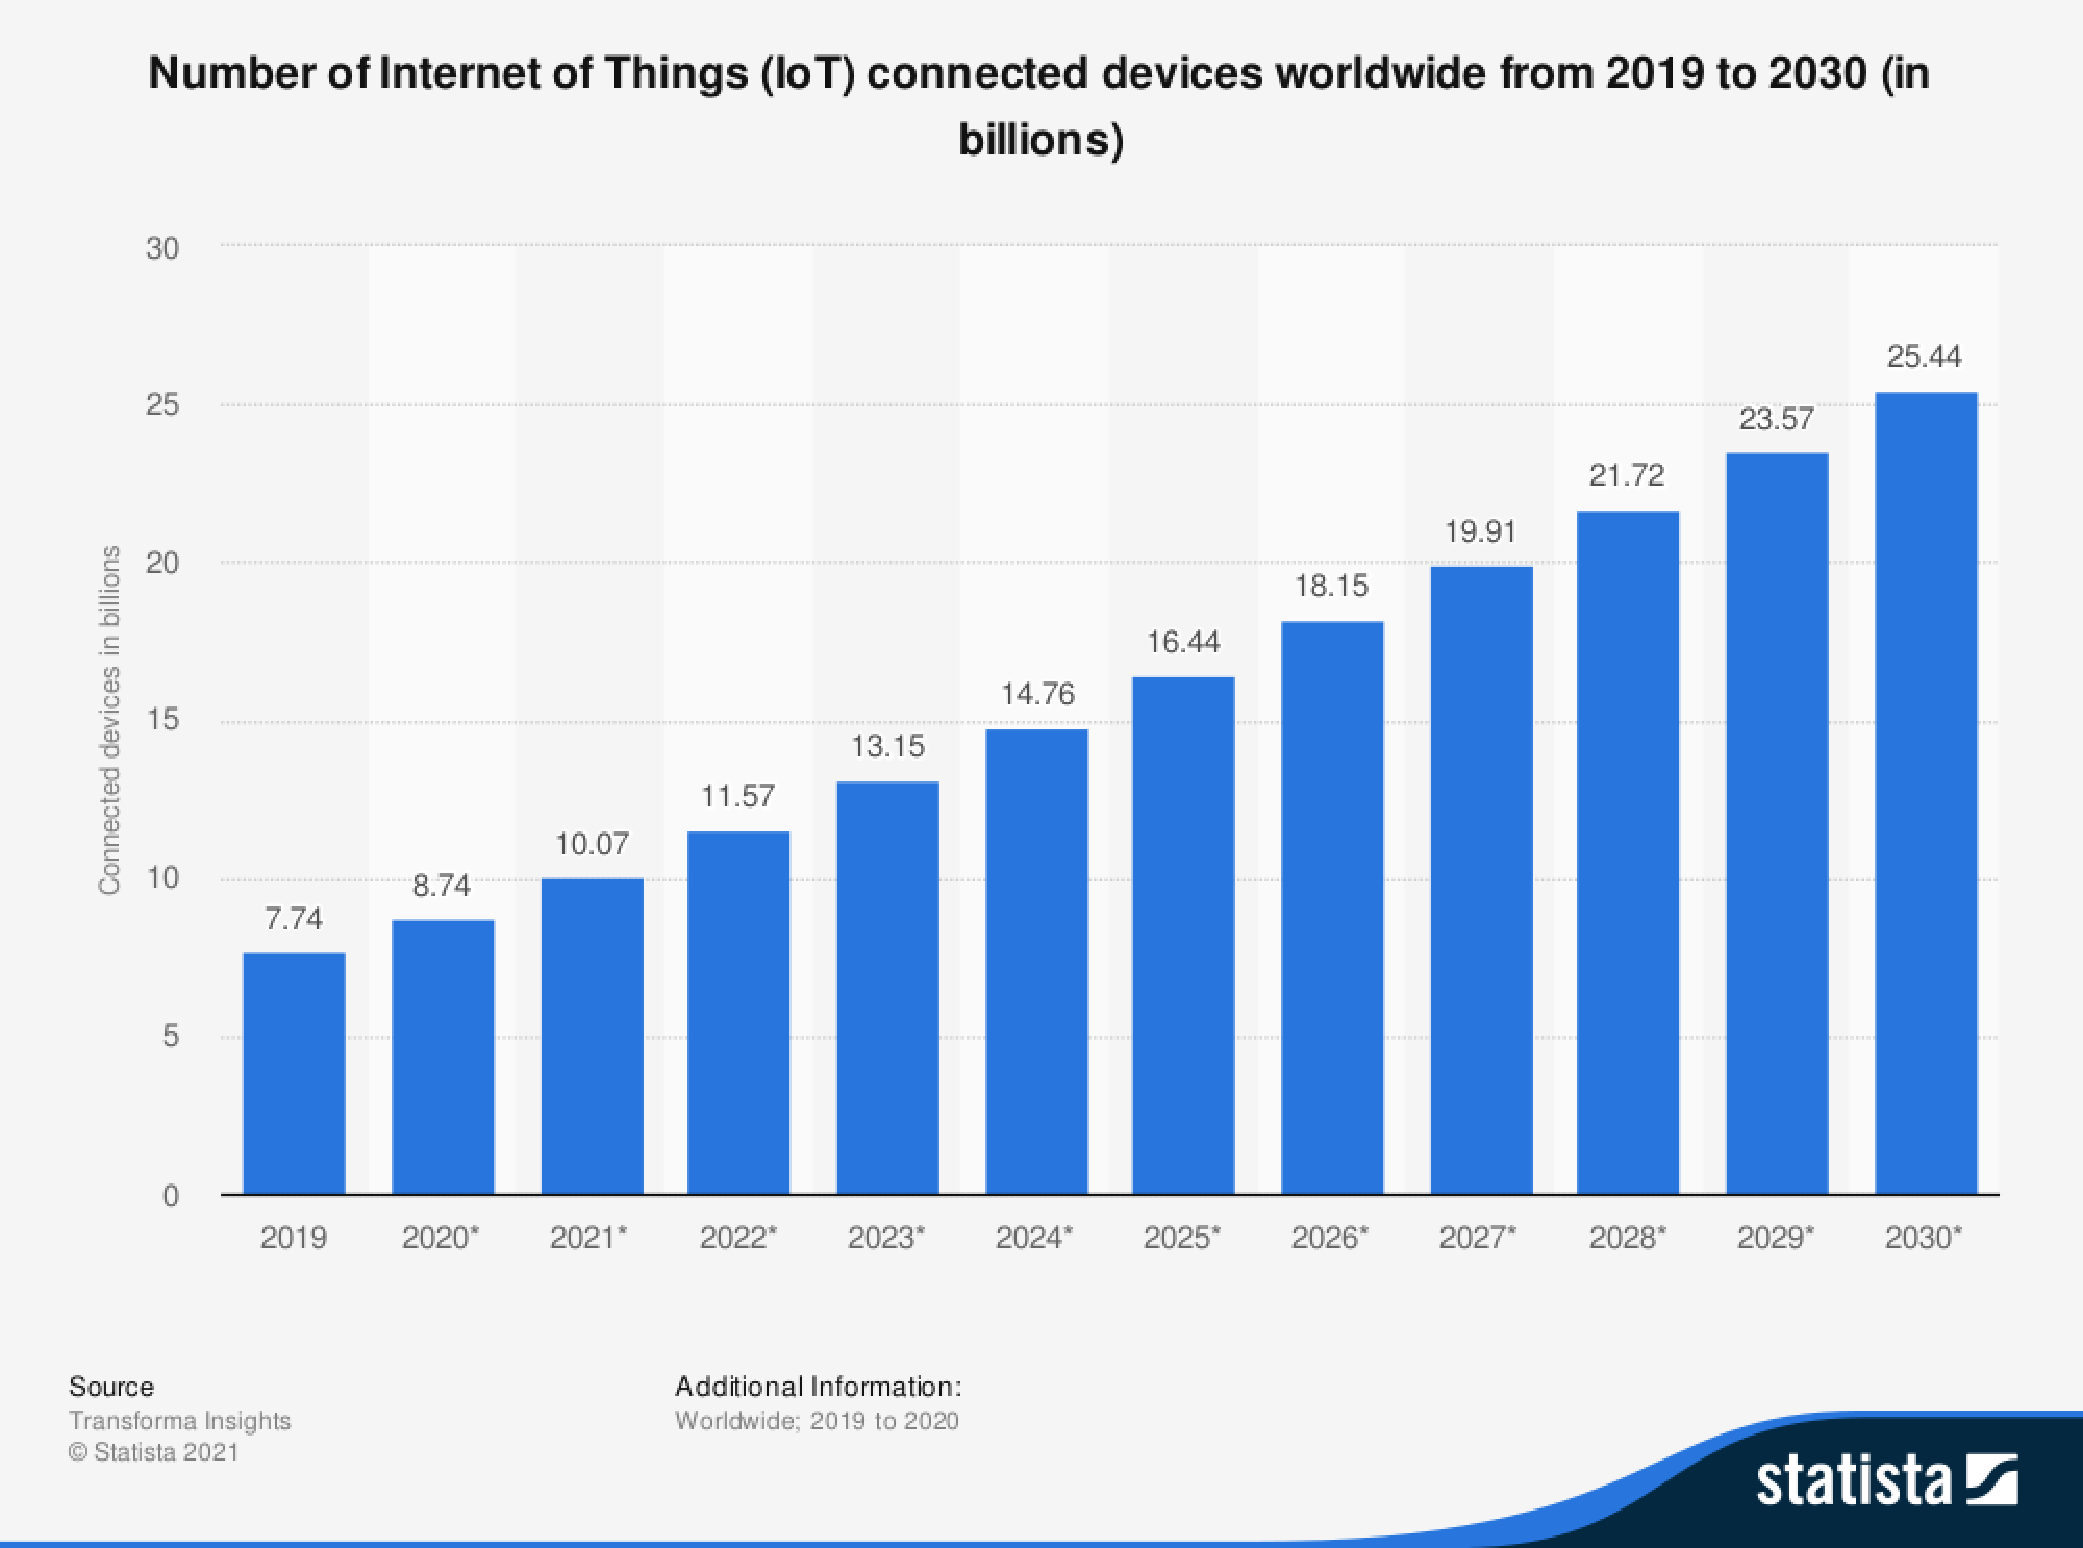
\includegraphics[width=0.8\textwidth]{assets/problem/statistic_id1183457_number-of-iot-connected-devices-worldwide-2019-2030.pdf}
    \caption{Number of IoT devices \cite{StatisticTransformaInsights}.}\label{fig:mumber_of_iot_devices}
\end{figure}

With the increasing amount of connected IoT devices, the data production increases too. Increase in data production also increases the demand to process the generated datasets. One conventional way  is the processing through cloud computing services. But this process generates significantly more pressure on the overall network and its bandwidth with increasing number of devices \cite{Yu2017}. For example, transmitting 1080p Video streams, in real time, from around 12,000 different devices requires a cloud ingress bandwidth of 100 gigabits per second. One million of these devices require 8.5 terabits per second. Sending the video streams to nearby processing platforms like edge computing platforms will reduce the overall bandwidth congestion \cite{Shi2016a}. 

\bigskip
Advantages like almost infinite computing power, unlimited storage capacity, dynamically scale your services or the fact of only paying what you use, the so-called pay-as-you-go model, has driven many businesses to migrate to centralized cloud approaches \cite{APOSTU2013}. Edge Computing on the other hand is a decentralized computing infrastructure. Disadvantages from cloud computing like privacy, security or compliance come out as a benefit on edge computing \cite{IndustrialInternetConsortium2018}. For example, edge computing infrastructures can enforce privacy policies of its owner by keeping the data inside the users trust domain\cite{Shi2016a}. Other advantages like masking cloud outages \cite{Shi2016a} can be also a benefit of moving to the edge. For example the recent incident at OVH Cloud in France destroyed an entire data center due to a fire, which resulted in an irreversible data loss for many businesses at once \cite{Holland2021}. Outages like the fire or other outages like network failures, denial-of-service attacks (DDoS) and more do not affect local edge computing infrastructures \cite{Shi2016a}. But more about the advantages of edge computing in the chapter \ref{chap:edge-computing}. 

\bigskip
Also, round trip times (RTT) to remote data centers are increased compared to local computation units. The most obvious about increased RTT is the physical distance. There is no way to get around the speed of light limitation. Another limiting factor is the node count and the congestion on each of the nodes the connection takes on its way \cite{Cloudflarea}. An example where high latency can be a problem are offshore oil rigs. Connecting oil rigs to the internet with under sea cables won’t be a financially viable option for the operators. Satellite connectivity is used to transfer data from oil rigs to the mainland \cite{HaglandHansen}. The RTT over satellite was measured to be around 880ms to 1243ms \cite{Bisu2018}. This high latency may be improved in the future by newer satellite installations like SpaceX’s Starlink constellation which aims to be as low as 20-40ms RTT. Starlink constellation is currently in a public beta testing phase \cite{Grush2020}. Latency is also affected by the bandwidth of each line between the nodes taken by the connection. The line with the smallest bandwidth is referred to as the bottleneck bandwidth. The rate of sending at the bottleneck affects the overall latency. The bottleneck bandwidth also indicates the maximum possible throughput \cite{Gettys2011}. The latency and bandwidth limits can be partially masked with sufficient effort and resource investment, like setting up a direct fiber cable connection to the nearest data center \cite{Shi2016a}.

\bigskip
One potential new requirement for some IoT devices is the near real-time capability, which is only possible due to the decrease in response time by a shorter traveling distance inside the system environment. A real life example of a big amount of data which needs to be processed near real time is the rise of the autonomous vehicle. Each of these autonomous vehicles has a lot of sensors and cameras on board whose data must be processed near real time to perform an appropriate response to the surrounding environment. Sending this data into the cloud as an unbound latency, hence we can not implement near real time application with a cloud component. Edge computing targets this need of processing data locally. No wonder that a number of commercial and open source edge platforms are out there to be chosen. 

\bigskip
To Sum it up so-called edge platforms can be used to simplify the distribution of workloads on the edge to meet the given requirements which the cloud and remote data centers can’t meet. 


%---- Evaluation Criteria
\chapter{Evaluation criteria}\label{chap:evaluation-criteria}
This chapter represents the criteria for the evaluation after the use case implementation in each edge computing platform. The order of the evaluation criteria is irrelevant. Some criteria maybe weighted differently depending on the use case and the specific needs of each project. At the end of this thesis, the evaluation will be based on a single use case for simplicity, but the criteria will be assessed as objectively as possible.

\subsubsection*{Access to peripheral devices}
In some cases access to peripheral devices is required to collect/send data to e.g. an attached camera, sensor or even hardware for accelerating computation like GPUs or TPUs for machine learning tasks. Therefore, the Platform should allow its nodes to access certain peripheral devices. In addition, there needs to be an option to target a specific edge node for an application deployment to meet requirements like the use of an TPU.

\subsubsection*{Data Persistence}
The generated data also needs to be stored, whether it is the produced data by e.g. sensors or the results of any local computation tasks. It’s also important to securely store the data. This includes encryption and redundancy. Redundancy is required to build robust \gls{IoT} applications, since every data storage outage can bring the complete application offline.

\subsubsection*{Development Environment}
The developers should be capable of running a smaller local development environments for testing, debugging and new feature implementation. Preferred a virtual environment which can be dynamically adjusted to prevent setting up a mirror of the full system.

\subsubsection*{Extensibility} 
Depending on use case, it is sometimes required to add new devices over time. Some reason could be a replacement of a worn out device or the extension of the existing system \cite{Shi2016b}.

\subsubsection*{Offline capability}
Sometimes edge computing is not just about moving the computation near to the user/devices, in some cases it is also about operating normally without reliable internet connection or even completely without any connection. For that, the edge platforms should operate normally without a stable or even without any connection. In addition, it should be noted whether the initial setup process needs a connection or not.

\subsubsection*{Cloud connectivity}
Integrated cloud connectivity could be advantageous for some use cases. Examples are things like sending locally computed data to the cloud for further analysis or monitoring.

\subsubsection*{Service Differentiation}
Some services may have different priorities depending on their purpose. For example, critical services such as things diagnosis and failure alarm should be processed earlier than ordinary services \cite{Shi2016b}. Critical services are determined by the use case and differ from use case to use case.

\subsubsection*{Reliability}
Reliability on the edge is a different challenge because more failures can occur. Failure can be more than just the application is repeatedly crashing. Additional failures can be worn out components, connection lose, power cord cut, battery outage and so on. To prevent failures, monitoring can be a benefit. The monitoring should include status information about any component in the system and network. Also, testing the data quality can be used to detect failures early for predictive maintenance \cite{Shi2016b}.

\subsubsection*{Security}
Focuses on the use of common encryption technologies or generally common solutions for IT security. Difficult to evaluate, so the basic things are discussed here. Examples would be the use of encryption technologies like \gls{TLS} and access control mechanisms. The focus should be on what encryption technologies are supported and used out of the box.

\subsubsection*{Real-time capability}
Real-time in this context is meant to provide low latency device to device or service to service communication, not the real-time of \gls{RTOS} systems. Some edge computing platform provide a built-in messaging solution to enable services to communicate with each other. These built-in solution should be evaluated about their overall latency and their capability of sending and delivering messages near real time. For this work we define near real time by means of an example. The example includes a camera as \gls{IoT} device. If this camera captures 30 \gls{FPS} the time until a response must be present is 33.33 milliseconds (\( \frac{1000ms}{30} = 33.33ms \)). By increasing captured frames per second to 60 \gls{FPS} the necessary response time decreases to 16.67ms (\( \frac{1000ms}{60} = 16.67ms \)). In summary, the near real time is defined so that a response is available before the next message arrives for processing.

\subsubsection*{Performance}
Edge devices are mostly not high-end power houses, on the contrary they are mostly very slow compared to virtual machines in the cloud. Therefore, edge platforms are restricted to less computational power than in the cloud. Besides the core platform services, the edge platform needs to provide enough resources to run the services for its use case. In general each edge platform should use as few resources as possible. More computing capacity left over logically means more resources are available for processing data.

\subsubsection*{Distributing workload}
Some services may not be intended for only one specific device, but can be run on multiple devices at the same time to reduce overall load. The platform should support the distribution of workload to its nodes. 

\subsubsection*{Energy Consumption}
In some cases a permanent power supply is not guaranteed, therefore a low power consumption of the overall system is an advantage.

\subsubsection*{Cost}
Won't cover the hardware cost because this is very individual to each use case or company. Costs are difficult to calculate because many individual projects of different sizes are created here. Therefore, this criterion only considers what needs to be taken into account in a cost calculation compared to, for example, a cloud infrastructure. For example potential cloud fees will be covered here.


%---- Basics
\chapter{Basics}

%%%%%%%%%%%%%%%%%%%%%%%%%%%%%%%%%%%%%%%%%%%%%%%%%%%%%%%%%%%%%%%%%%%%%%%%%%%%%%%%%%%%%%%%%%%%%%%%%%%%%%%%%%%%%%%%%%%
\section{MQTT}
\gls{MQTT} was developed by Stanford-Clark of IBM and Arlen Nipper of Arcom Control Systems Ltd (Eurotech) in 1999. It is one of the oldest machine to machine communication protocols. It is a publish/subscribe model for lightweight communications between devices \cite{Naik2017}. A \gls{MQTT} setup consists of two components. A broker, in the standard referred to as “server”, which acts as a bridge between the publishers and the subscribers and a \gls{MQTT} client which acts as publisher, subscriber or both \cite{OASIS2019} \cite{Naik2017} \cite{Bandyopadhyay2013}. Figure \ref{fig:mqtt-architecture} shows a basic architecture of one broker, one publisher and a subscriber which can also publish messages. Messages, produced by the publisher, are sent to the broker. Every message is published to an address known as topics. Topics use a hierarchical structure. The Subscribers can subscribe to one or more of these topics to receive published messages \cite{Bandyopadhyay2013}.

\begin{figure}[H]
    \fontsize{9}{10}\selectfont
    \centering
    \def\svgwidth{\textwidth}
    \input{assets/basics/MQTT.pdf_tex}
    \caption{Basic MQTT architecture.}
    \label{fig:mqtt-architecture}
\end{figure}

Each Subscriber can define a \gls{QoS} level on their subscription to a topic. The different QoS levels determine the reliability of receiving messages as subscriber \cite{OASIS2019}. The three quality of service levels (\gls{QoS}) for delivering messages are: \cite{OASIS2019} 

\begin{itemize}
    \item \textbf{QoS 0:} At most once, will send the message only once without any acknowledgement. Messages may not arrive.
    \item \textbf{QoS 1:} At least once, ensures the message is received at least once by the subscriber. Duplicates are possible.
    \item \textbf{QoS 2} Exactly once, ensures the message will be received exactly once by the subscriber. No Duplicates compared to QoS 1.
\end{itemize}

The \gls{MQTT} protocol uses TCP with optional TLS/SSL, for security, as a transport protocol. It is also possible to establish a connection with WebSockets \cite{OASIS2019}. The transferred data is in binary format and is capped to a maximum payload size of 256 megabytes \cite{Naik2017}.

%%%%%%%%%%%%%%%%%%%%%%%%%%%%%%%%%%%%%%%%%%%%%%%%%%%%%%%%%%%%%%%%%%%%%%%%%%%%%%%%%%%%%%%%%%%%%%%%%%%%%%%%%%%%%%%%%%%
\section{Container}
A container is a unit of software that packages code and all its dependencies to run quickly and reliably on any computing environment \cite{dockerWhatDocker}. Each container needs a runtime to run on. There are different container runtimes available out there. Runtimes like Docker or the containerd, which was split off from Docker, let the developer run container images by unpacking them and starting the process \cite{Lewis2018}.

\bigskip
On the 22nd of June in 2015 leaders of the container industry like Docker, CoreOS and others established the \gls{OCI} a lightweight, open governance structure (project), formed under the auspices of the Linux Foundation, for the express purpose of creating open industry standards in the container format and runtime environment. A cornerstone was laid by Docker upon contributing its own container format and runtime, runC, to the \gls{OCI} \cite{TheLinuxFoundation}. Currently, there are two specifications available: \cite{TheLinuxFoundation}
\begin{itemize}
    \item Image Specification (image-spec): specifies how the image is structured
    \item Runtime Specification (runtime-spec): specifies how to run a “filesystem bundle” (image) that is unpacked on disk
\end{itemize}

\bigskip
Container orchestration systems like Kubernetes can then be used to serve fleets of containers which get automatically deployed, scaled and managed by a container orchestrator \cite{TheKubernetesAuthors}.

%%%%%%%%%%%%%%%%%%%%%%%%%%%%%%%%%%%%%%%%%%%%%%%%%%%%%%%%%%%%%%%%%%%%%%%%%%%%%%%%%%%%%%%%%%%%%%%%%%%%%%%%%%%%%%%%%%%
\section{Cloud Computing}
Cloud computing is shaping the IT Industry by how hardware is designed and purchased. For example developers, start-ups or companies can come up with a great idea and won't be required to buy hardware to run their idea. There is no need for a large capital to invest into hardware and no need of operating and maintaining the hardware. The fact of over-provisioning or under-provisioning is also eliminated, as cloud computing can be scaled according to demand and without any upfront investment \cite{Armbrust2010}. Today public cloud providers like \gls{AWS}, Microsoft Azure or \gls{GCP} offer the pay-as-you-go pricing model where you only pay the resources you are really using \cite{AWSWhatComputing} \cite{MicrosoftWhatAzure} \cite{GoogleCloudCloud}. This pricing model then allows ideas to be implemented without the need of a large capital like what was previously mentioned.

%%%%%%%%%%%%%%%%%%%%%%%%%%%%%%%%%%%%%%%%%%%%%%%%%%%%%%%%%%%%%%%%%%%%%%%%%%%%%%%%%%%%%%%%%%%%%%%%%%%%%%%%%%%%%%%%%%%
\section{Internet of Things}
The term \gls{IoT} was first mentioned by Kevin Ashton in 1999 in the context of supply chain management \cite{ashton2009internet}. However, in the past decades, the definition has been evolved to cover a wide range of applications like healthcare, utilities, transport, etc. \cite{Lee2015}. Like the problem chapter \ref{chap:problem} already introduced the raising amount of \gls{IoT} devices across the world shows big interest in this paradigm. \gls{IoT} is about a technology paradigm of a global network where devices are connected with each other. The devices are capable of interacting inside this network with other devices \cite{Lee2015}. These devices are mostly very small and have the ability to sense, compute, and communicate wirelessly in short distances. Today they are used in a wide range of applications like in environmental monitoring, infrastructure monitoring, traffic monitoring, retail and more. Cloud computing will then receive these data for further processing or other processes \cite{Gubbi2013}. In the edge computing context, \gls{IoT} devices connect to the edge computing platform and not to the cloud computing platform for further processing the produced data.


%---- Edge Computing
\chapter{Edge Computing}\label{chap:edge-computing}
Edge Computing started back in the 1990s when Akamai introduced the first content delivery network (CDN) for accelerating the overall web performance. It is still used today for bringing web content closer and faster to the user. For this, nodes are distributed away from the computing center to be closer to the user or end-device. Thought further edge computing extends the CDN concept by adding cloud computing concepts. Therefore, edge computing is no longer bound to caching web content and can now also be used for arbitrary code execution. To get more benefits out of edge computing, the computing tasks can be moved even further to the user or end-device \cite{Shi2016a}. This tackles various problems which occurred with the recent move to the cloud. The following gives a brief overview which problems get tackled and what are the advantages of doing edge computing.

\bigskip
A very simplified and common architecture of edge computing is shown in figure \ref{fig:hierarchical-cloud-edge-iot}. The lower rectangle represents the \gls{IoT} devices, which can be anything from environmental sensors to video cameras. These devices connect them self to the nearest available edge node of the system. The next level is the edge nodes which do the processing for the IoT devices. Results, gathered by the edge processing of data can then be sent to the cloud, the top most rectangle.

\begin{figure}[H]
    \centering
    \fontsize{9}{10}\selectfont
    \def\svgwidth{\textwidth}
    \input{assets/edge-computing/Cloud-Edge-IoT.pdf_tex}
    \caption{Hierarchical structure of Cloud and Edge computing (Figure adapted from \cite{Infineon2019}).}
    \label{fig:hierarchical-cloud-edge-iot}
\end{figure}

\bigskip
\paragraph{Highly responsive:} The IoT device mostly isn't powerful enough to run the computing process on their own, so they have to send it to a more powerful machine. The default strategy is mostly to offload the task to a cloud infrastructure. But offloading the computing task to a cloud infrastructure comes with some problems in the latency section. With increasing physical distance the latency is also increasing and most of the time the data center isn't next to the sensor device. Edge computing can tackle this by moving the computing near to the sensor device which reduces the overall physical distance and therefore the latency which is added just due to the physical distance \cite{Shi2016a}.

\paragraph{Data Privacy:} Growing concerns about data privacy can be mitigated by shifting the processing of sensitive data closer to the user or factory. With edge computing, the data can be processed inside the owner's trust domain which allows the owner fine grain control about his data. A simple example about how edge computing can protect the owners' privacy is a video camera which sends its captured frames to a data center for evaluation. By doing the evaluation inside the owner's trust domain, in our case edge computing, privacy can be sustained \cite{Shi2016a}.

\paragraph{Masking cloud outages:} Cloud outages like the recent outage at Fastly CDN or the fire at the OVH cloud in France made many services unavailable around the world \cite{Rockwell2021} \cite{Holland2021}. Cloud outages can have different kinds of nature. Wrong configuration, fire, natural disasters, cyberattacks, terrorist attacks, weak networking infrastructure and more. By staying away from the cloud, outages like these won't affect your system. Of course, there are use cases where even the edge computing platform sends its aggregated results to the cloud, but a temporary outage of a cloud can be easily masked by resending the results upon reconnection \cite{Shi2016a}.

\paragraph{More sustainable future:} Data centers consume a lot of energy which generates carbon emissions during production. Even the positive trend of using renewable energy only for operating data centers, an even more sustainable approach can be done by reducing the overall traffic to and from the data centers. Edge Computing can help to greatly reduce the bandwidth usage to cloud data centers by computing the data locally and only sending the relevant data like results or aggregated data to the cloud. It can even completely eliminate any bandwidth usage outside the edge computing network if the use case allows operation without any internet connection or cloud computing support. Even the use of existing hardware is more sustainable. Many existing devices are already capable of doing computational task. Many existing devices have enough computational power for some computational tasks, but this power is mostly not used at all. These underused devices is a waste of potential and resources \cite{ObjectBoxLimited2021} \cite{Adib}.

\paragraph{Scalability:} By doing the processing at the edge not only latency can be reduced also ingress bandwidth to the cloud can be reduced. By processing the data near the user and only sending the results to the cloud, the ingress bandwidth to the cloud can be reduced by a magnitude of three to six orders. A video camera is one example where the bandwidth usage can be extraordinarily high. For example, 12,000 users transmitting a 1080p video would require a link of 100 gigabits per second; a million users would require a link of 8.5 terabits per second. This tremendous amount of bits per second can saturate a metropolitan area network. By offloading the computation of these video streams to nearby edge nodes the bandwidth can be reduced dramatically \cite{Shi2016a}.

\section{Edge and Fog Computing}
By doing some research about edge computing the word combination fog computing, often appears alongside the word combination edge computing. This section covers the subject of the relation between edge and fog computing. By digging into several papers and blog articles the authors come to a different conclusion about the difference between edge and fog computing. Some authors come to the conclusion that fog computing has cloud-like structures. Fog computing structures can be seen as an extra hierarchical layer between cloud and end devices. This additional layer is located in the local network and acts as a preprocessor of the locally collected data. These authors then describe edge computing as a model of directly processing the data on the devices themselves or very close next to them \cite{Ulmen2019}. In conclusion, these authors see fog computing as a kind of micro local data center and edge computing as an on-device computing solution. On the other hand, Cisco defines fog computing as a subtype of edge computing. For them, fog computing refers to decentralization method where nodes get strategically placed between the cloud and edge devices as the other authors do. The only difference is that fog computing is grouped under edge computing \cite{Cisco}. Even the edge computing platforms themselves show that there is no agreement on how edge or fog computing are grouped exactly. For example, the eclipse foundation calls their edge computing platform ioFog \cite{EclipseFoundation}, which hints at fog computing with just its name. On the other hand, the Linux foundation refers to edge computing with its lightweight Kubernetes platform called k3s. Both ioFog and k3s, use similar concepts that why they can be compared here but more about these similar concepts later on \cite{k3s}. For this thesis, we stick to the classification of Cisco where fog computing is a subtype of edge computing.

\section{Summary}
In general, edge computing is the process of performing common cloud computing tasks closer to the user or target devices. The increasing amount of IoT devices and the associated network and computation problems led away from the centralized cloud approach to a decentralization like edge computing \cite{Shi2016a} \cite{Yu2017}.


%---- Implementation
\chapter{Edge Computing platforms}
This chapter covers the three selected edge computing platforms which get evaluated on the basis of a use case implementation which is also described here. Besides the edge platforms, the entire experiment and the used resources and everything which belongs to this is explained here.

\section{Use case}
In order to be able to carry out an evaluation of the three selected platforms, a specific application is built as identically as possible in all platforms. The chosen use case should represent a facility with different services. The system to be implemented only represents a subsystem of these services. This subsystem should contain a kind of emergency service which responds to certain emergency scenarios like increased temperature or gas detection by enabling/disabling ventilation devices. Also the monitoring of entire system should be given by collecting, storing and visualize all produced data. This subset is chosen to show different kinds of workloads and how each platform will handle it. To get a better overview of the given platform, mainly built-in features should be used, if possible.

\bigskip
The following figure \ref{fig:use-case-overview} shows the context view of each edge platform and the supporting systems around it. The blue block in figure \ref{fig:use-case-overview} represents one of the three edge platforms which gets implemented in later sections. The purple block represents the optional cloud support. The gray blocks refer to sensors and actors which produce or consume data from the connected edge platform. User interaction is also given by either the edge platform itself or the optional cloud environment.

\begin{figure}[H]
    \centering
    \fontsize{8}{10}\selectfont
    \def\svgwidth{\textwidth}
    \input{assets/use-case/architectural-overview.drawio.pdf_tex}
    \caption{Use case system overview.}
    \label{fig:use-case-overview}
\end{figure}

\section{Setup}
For the use case implementation different sensors, actors and software packages were developed. This section covers the respective use of each sensor, actor and software package. Some software packages will be at a later point in time to match the different edge computing platforms. But the core functionality while remain for each software package.

\subsection{Compute units}\label{subsec:compute-units}
For this experiment, up to three Raspberry Pi's and one external \gls{tpu} are available. The chosen \textit{Raspberry Pi 4 Model B} is equipped with 4 GB of \gls{RAM}. The Raspberry Pi's are referred to as nodes of the edge computing system. Each node is powered by \gls{PoE}. Each node has an official Raspberry Pi \gls{PoE} hat mounted on top. Also, each node has a passive cooled enclosing. One \textit{TP-Link TL-SG1005P} 5-Port Gigabit PoE Switch provides the power and the connection to the router. Each node is connected to the switch via a \textit{CAT 6} network cable. For connecting the sensor to the system, an WiFi \gls{AP} is provided. Figure \ref{fig:network-topology} shows the overall network topology of the three nodes.

\begin{figure}[H]
    \fontsize{9}{10}\selectfont % <-- adjust font in svg
    \centering
    \def\svgwidth{\textwidth}
    \input{assets/setup/compute-units_wiring.drawio.pdf_tex}
    \caption{Network topology.}
    \label{fig:network-topology}
\end{figure}

The network has an internal and external bandwidth bottleneck. The internal bottleneck refers to the connection between the router and the first switch, which is limited to 1 Gbit/s. The external bottleneck is limited by the booked data usage plan of 100 Mbit/s. These bottlenecks then results in an internet download bandwidth of 100 Mbit/s and an internal data transfer rate of 1 Gbit/s.

\bigskip
It should be noted the software packages which will run on the edge computing platforms need to be cross compiled to match the Raspberry Pi's processor architecture. Each Raspberry Pi comes with a quad-core \textit{Cortex-A72 (ARM v8)} processor \cite{Raspberrypifoundation}. Due to the fact that the used processors in this experiment are ARM based (\ref{subsec:compute-units}) the container images or any other executable must be compiled to run on ARM devices. To be more clearly, the cross compile target platform is `linux/arm64/v8` for the Raspberry Pi's running Ubuntu 20.04 ARM in 64 Bit.


\subsection{BMP 280 Sensor}\label{subsec:bmp280}
The BMP 280 is a sensor which provides environmental data like temperature, pressure and altitude over I2C or SPI \cite{Az-delivery-BMP280}. The following setup explains how the sensor device for temperature, pressure and altitude was implemented. Next to the BMP 280 the microcontroller ESP32 Dev Kit C V4 was used to read and transfer the data via MQTT to the nearby edge computing platform. The application, running on the ESP32, was build inside Microsoft’s Visual Studio Code editor in conjunction with the PlatformIO extension. For simplification purposes the initial application was generated, configured and implemented inside a PlatformIO project. PlatformIO provides developers with tools to write applications for embedded products in a cross-platform, cross-architecture and multiple framework way \cite{Platformio}. The software for gathering and sending the data to the edge platform uses the Arduino framework. 

\bigskip
For talking to the BMP 280 sensor the C++ library from Adafruit \cite{Adafruit} was used. The used BMP 280 sensor from AZ-Delivery is only partially compatible to the Adafruit BMP 280 library \cite{Az-delivery-BMP280}. To work correctly the I2C address had to be changed to 0x76 instead of 0x77 in the header file.
 
\bigskip
The following figure \ref{fig:wiring-bmp280} shows the wiring of the BMP 280 to the ESP32 microcontroller. The wiring also includes LEDs which visually presents the connection status of the ESP32 to the Wi-Fi network and to the programmed MQTT broker. Figure \ref{fig:bmp280} show the wiring of Figure \ref{fig:wiring-bmp280} twice in real life.

\begin{figure}[H]
    \centering
    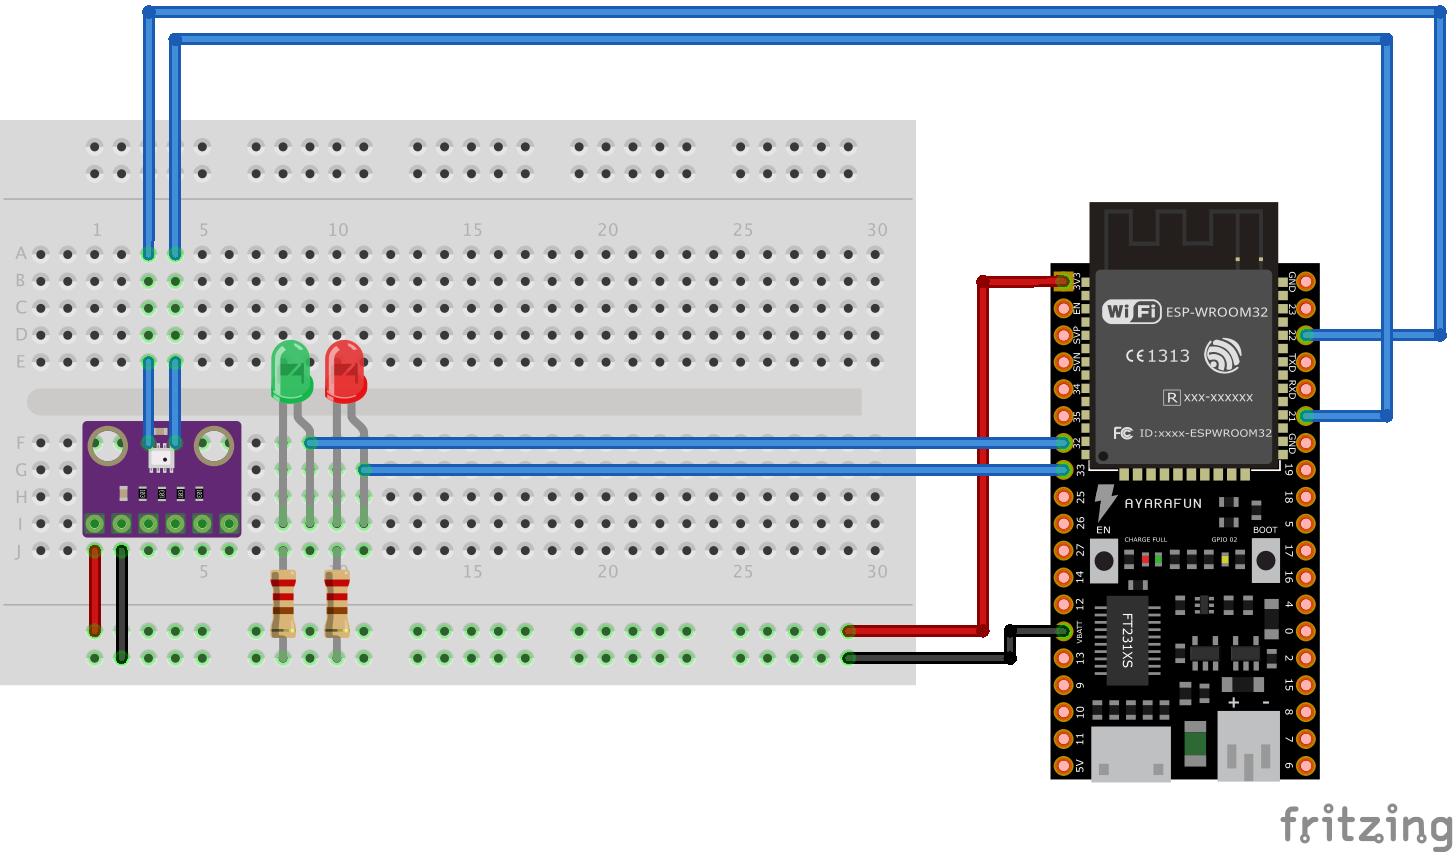
\includegraphics[width=\textwidth]{assets/setup/wiring-bmp280.png}
    \caption{BMP 280 wiring to the ESP32.}\label{fig:wiring-bmp280}
\end{figure}

\begin{figure}[H]
    \centering
    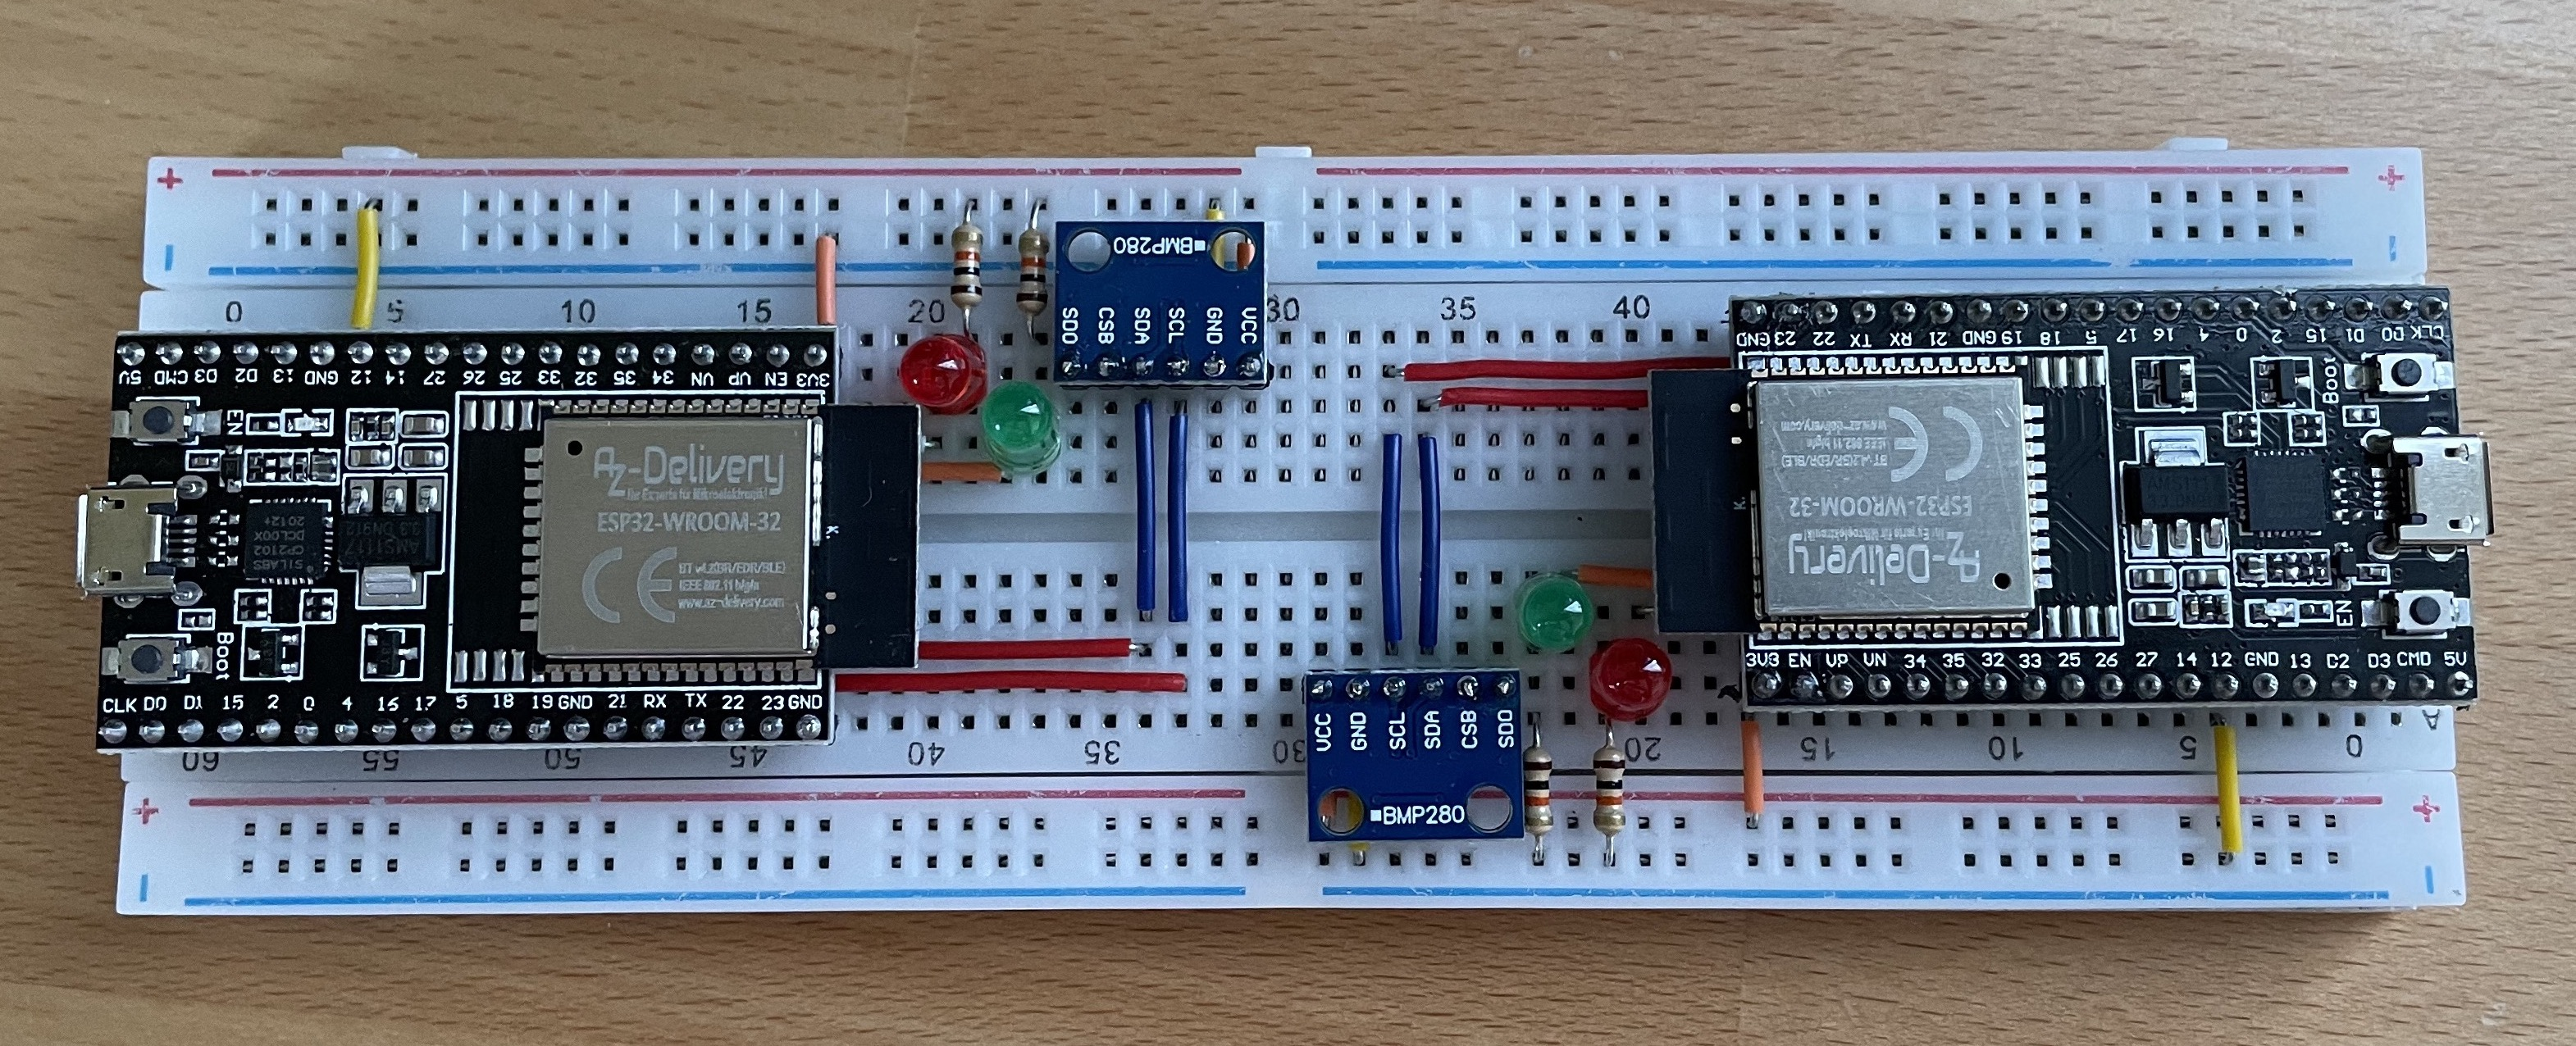
\includegraphics[width=\textwidth]{assets/setup/bmp280.jpeg}
    \caption{Real breadboard of two BMP 280 wired to their ESP32.}\label{fig:bmp280}
\end{figure}


\subsection{MQ-2 gas sensor}\label{subsec:mq2}
The MQ-2 is a sensor which detects LPG, i-butane, propane, methane, alcohol, hydrogen and smoke in the surrounding environment \cite{Az-delivery-MQ-2}. The following setup explains how the sensor device was implemented. Next to the MQ-2 the microcontroller ESP32 Dev Kit C V4 was used to read and transfer the data via MQTT to the nearby edge computing platform. The application, running on the ESP32, was built with the same tools as the BMP280 sensor (VS Code Editor and PlatformIO).

\bigskip
For talking to the MQ-2 sensor no library is required. The microcontroller only needs to read one digital and one analog pin. The digital pin provides information about whether gas is in the sensor environment or not. The analog pin returns a percentage value of the gas in the air.

\bigskip
The following figure \ref{fig:wiring-mq-2} shows the wiring of the MQ-2 sensor to the ESP32 microcontroller. Figure \ref{fig:mq-2} show the above wiring of Figure \ref{fig:wiring-mq-2} twice in real life.

\begin{figure}[H]
    \centering
    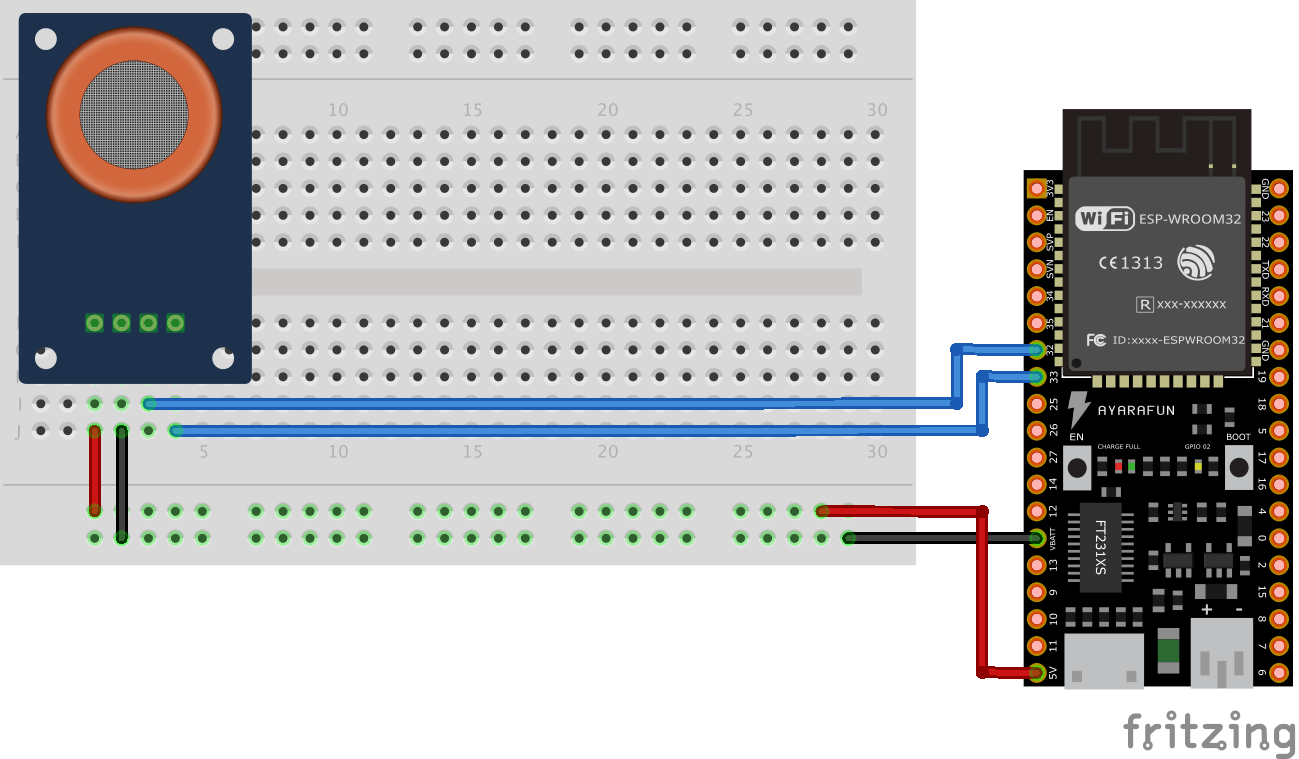
\includegraphics[width=\textwidth]{assets/setup/wiring-mq-2.png}
    \caption{BMP 280 wiring to the ESP32}\label{fig:wiring-mq-2}
\end{figure}

\begin{figure}[H]
    \centering
    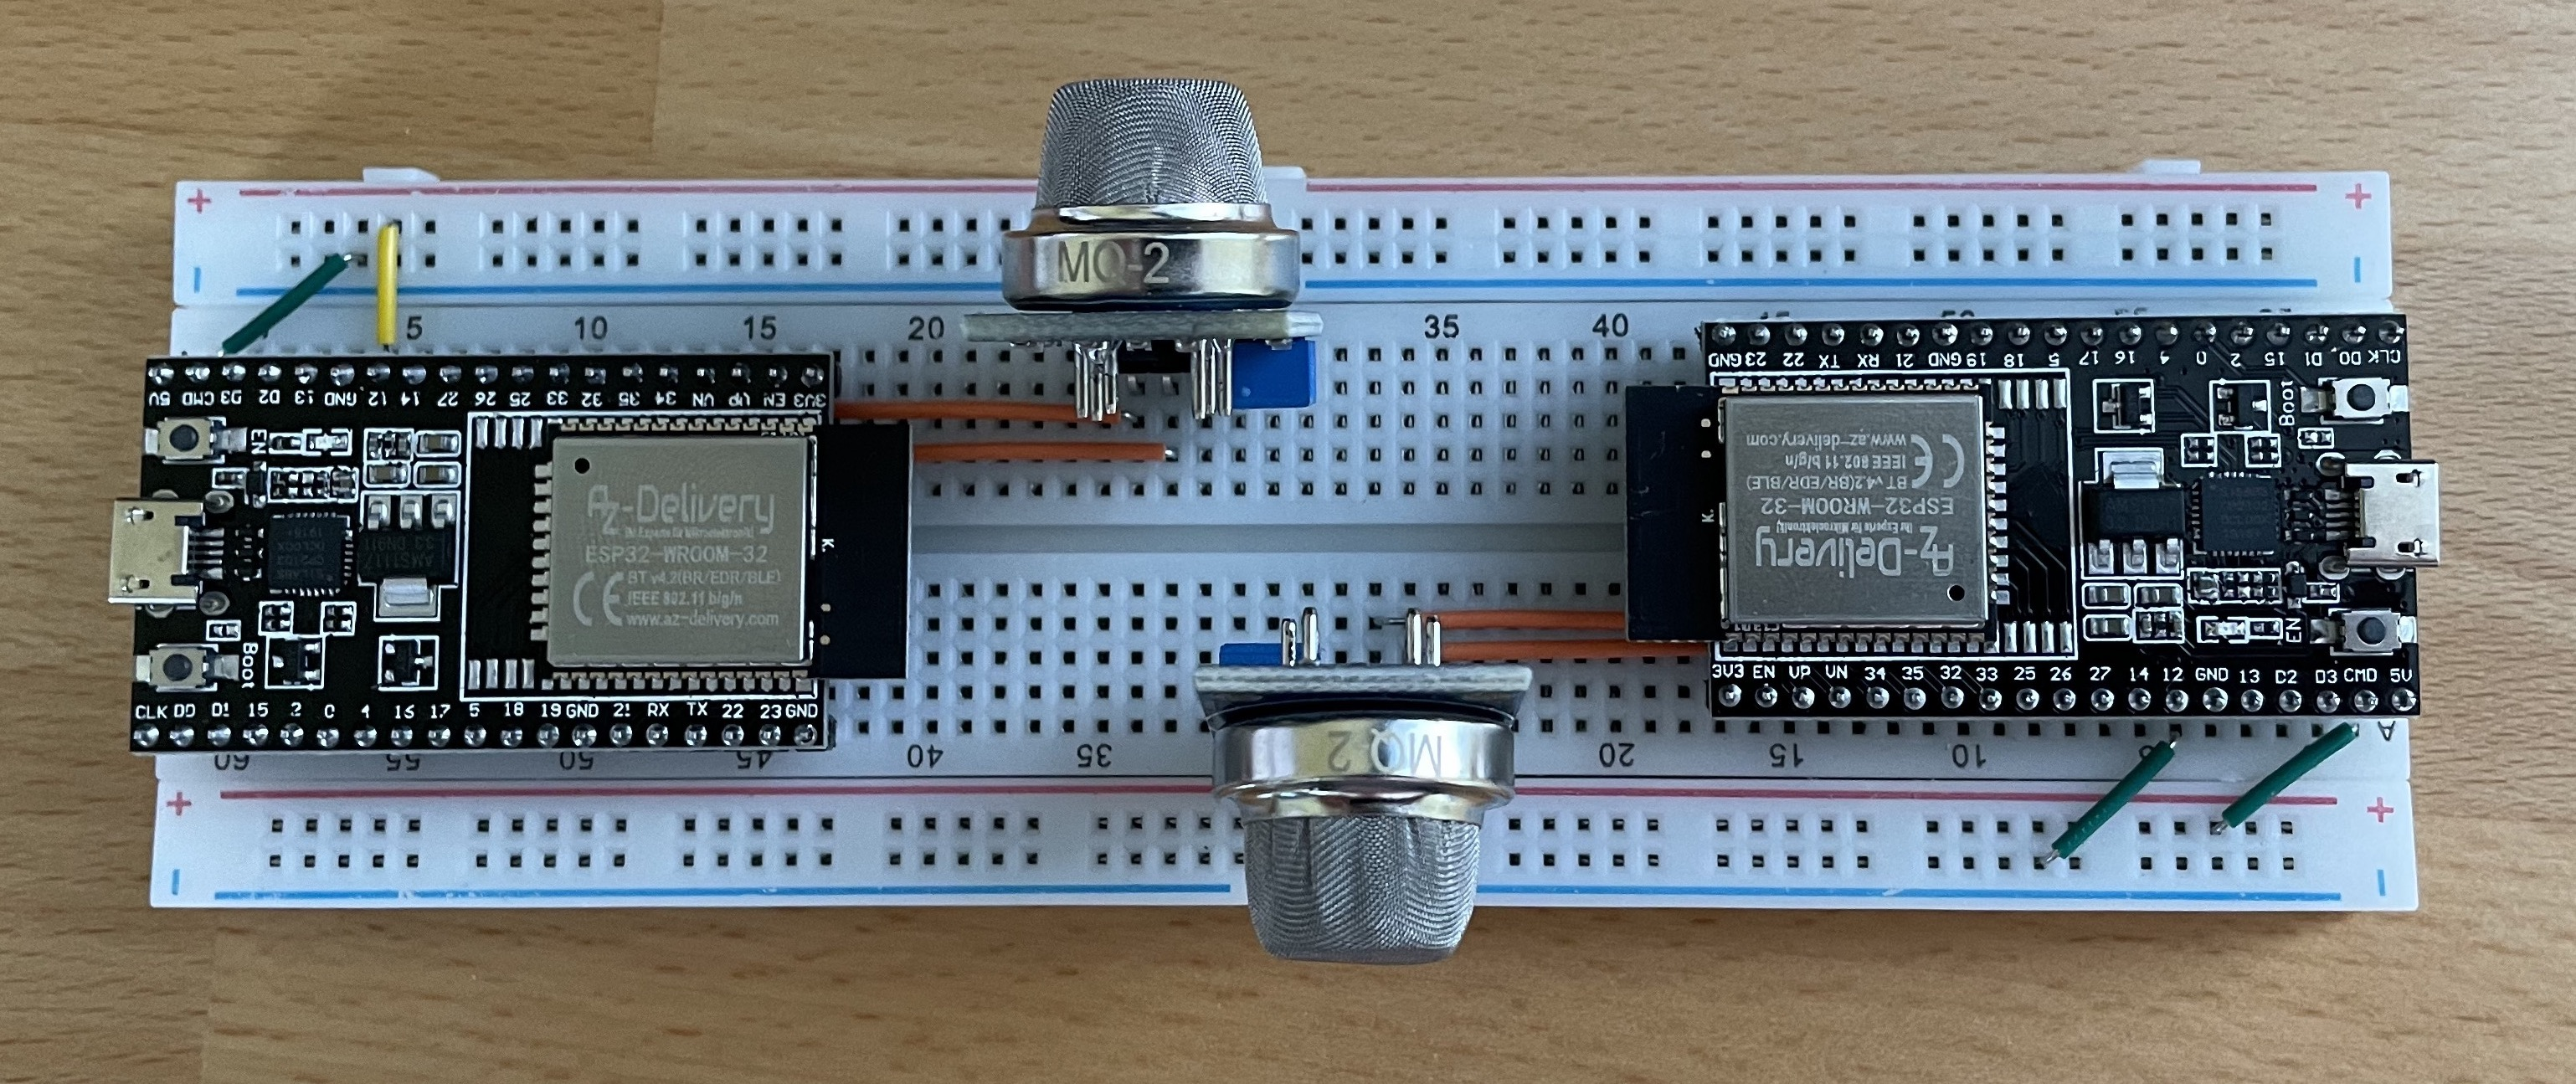
\includegraphics[width=\textwidth]{assets/setup/mq-2.jpeg}
    \caption{Real breadboard of two BMP 280 wired to their ESP32.}\label{fig:mq-2}
\end{figure}

Its also worth noting the MQ-2 sensor must settle for some time until credible data is generated. Figure \ref{fig:mq-2-percent-drop} shows the drop on gas percentage in the air over 30mins.

\begin{figure}[H]
    \centering
    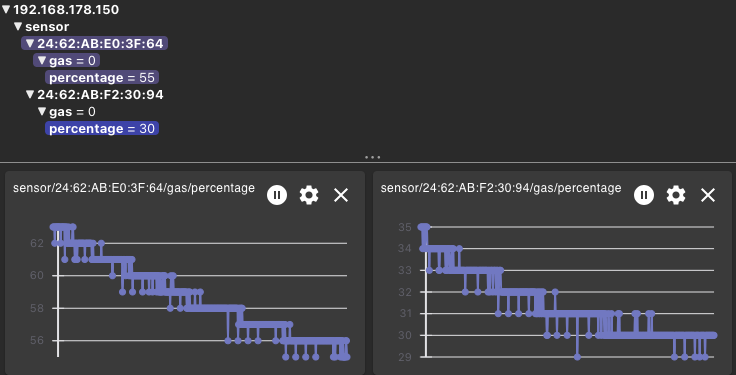
\includegraphics[width=\textwidth]{assets/setup/mq-2-percent-drop.png}
    \caption{Gas percentage drop over a 30min period.}\label{fig:mq-2-percent-drop}
\end{figure}


\subsection{Ventilation control}\label{subsec:ventilation}
This simple device controls a ventilation for venting in the event of the occurrence of hazardous gases or high temperature. This device does not detect the gas itself it just controls the ventilator. The used, two pin, ventilator model YDL3007C05 can be operated between 3.3V and 5V which is optimal to directly attach it to a microcontroller like an ESP32 or ESP8266. For this project an NodeMCU Lolin V3 Module ESP8266 ESP-12F \cite{Az-delivery-ESP8266} was used to start and stop the ventilator accordingly to the published states from a configured MQTT broker.

\bigskip
The application, running on the ESP8266, was built with the same tools as the devices described in previous sections (VS Code Editor and PlatformIO). The used framework was also the Arduino framework. For controlling the ventilator no specific library is required. The microcontroller only needs to set one GPIO pin to high for on or low for off.

\bigskip
The following figure \ref{fig:wiring-ventilator} shows the wiring of the ventilator to the ESP8266 microcontroller. Figure \ref{fig:ventilator} show the above wiring of Figure \ref{fig:wiring-ventilator} in real life.

\begin{figure}[H]
    \centering
    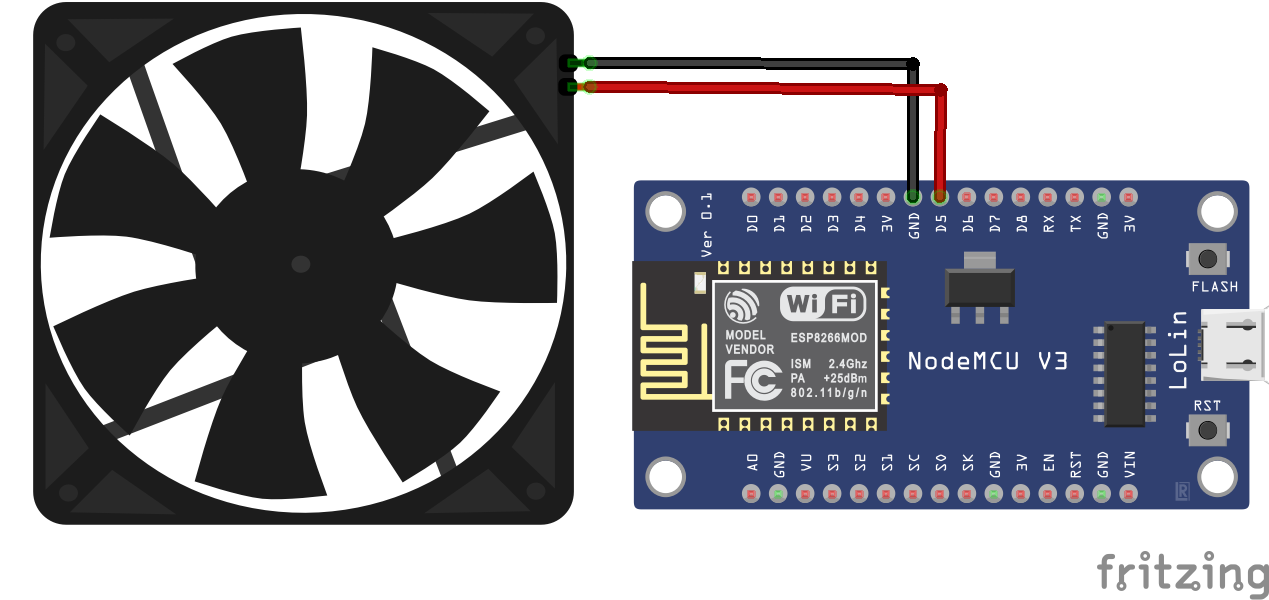
\includegraphics[width=\textwidth]{assets/setup/wiring-ventilator.png}
    \caption{Ventilator wiring to the ESP8266.}\label{fig:wiring-ventilator}
\end{figure}

\begin{figure}[H]
    \centering
    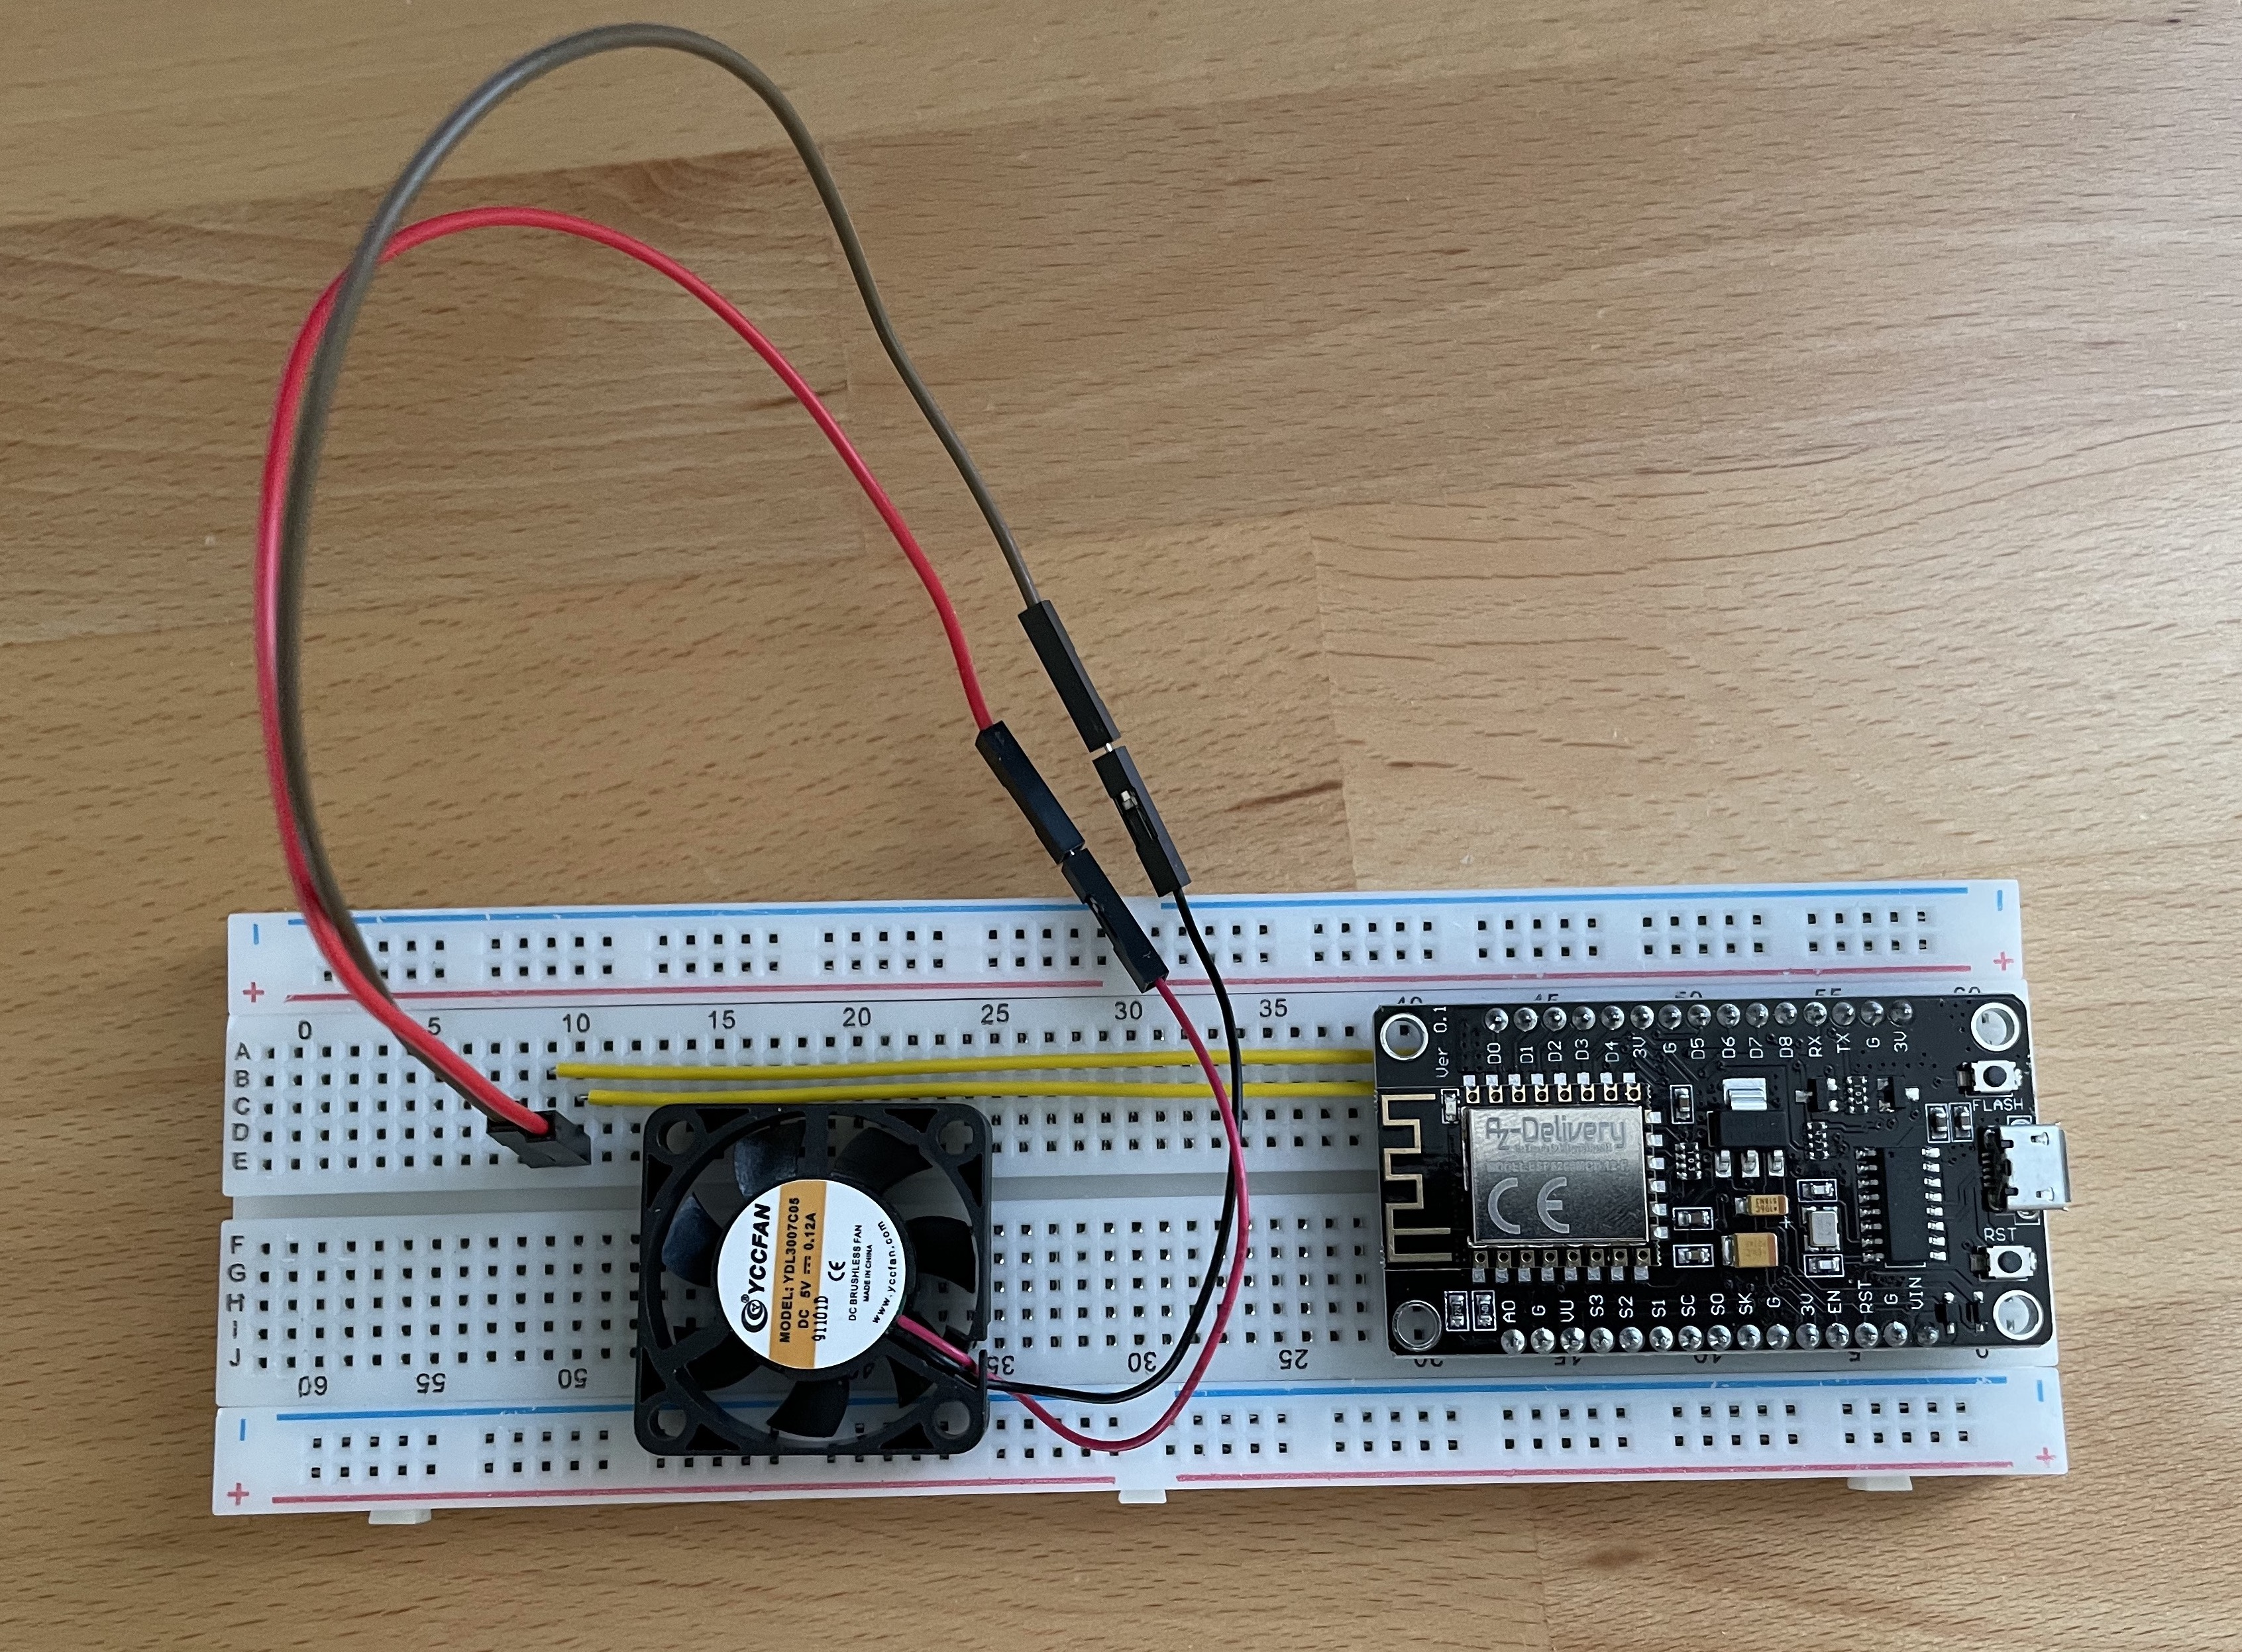
\includegraphics[width=\textwidth]{assets/setup/ventilator.jpeg}
    \caption{Real breadboard of ventilator wired to its ESP8266.}\label{fig:ventilator}
\end{figure}


\subsection{Camera sensor}\label{subsec:camera-sensor}
The setup also includes a camera that captures images for later processing with machine learning models (processing in section \ref{subsec:detector-service}). The camera sensor is represented as a combination of the official PiCamera and a Raspberry Pi 3B+. The python program, running on the Raspberry Pi, takes pictures in a predefined period and encodes them to a base64 string. The encoded string is then published to a given topic inside the MQTT broker of the connected edge platform for further processing by other services inside the system (see \ref{subsec:detector-service}).

%%%%%%%%%%%%%%%%%%%%%%%%%%%%%%%%%%%%%%%%%%%%%%%%%%%%%%%%%%%%%%%%%%%%%%%%%%%%%%%%%%%%%%%%%%%%%%%
% Services
%%%%%%%%%%%%%%%%%%%%%%%%%%%%%%%%%%%%%%%%%%%%%%%%%%%%%%%%%%%%%%%%%%%%%%%%%%%%%%%%%%%%%%%%%%%%%%%
\subsection{Detector service}\label{subsec:detector-service}
Detector is a service that further processes the data provided by the camera sensor of section \ref{subsec:camera-sensor}. The special feature of this service is the processing of the data by a \gls{tpu}. This \gls{tpu} is a piece of additional hardware attached via \gls{usb} to one of the nodes. The camera detection service is a small Python program which runs a MQTT client for subscribing to the corresponding topic. Received messages on the subscribed topic will then be base64 decoded and subsequently passed to the image detection, which runs a machine learning model (TensorFlow Lite model) on the attached \gls{tpu}. Results from the machine learning inference will then be published back into the system via an MQTT topic. For simplicity, an already trained model is used. The used model is a Mobile net v2 which detects different kinds of parrots. This model can be replaced with any image recognition model in the TensorFlow Lite format.

\subsection{Emergency service}\label{subsec:emergency-service}
The emergency service has the responsibility to avoid hazards regarding fire, explosions or high temperature. By monitoring the values of the BMP280 and MQ2 sensors the service will initiate countermeasures on any sign of gas or high temperature. To accomplish this the service will subscribe to the corresponding MQTT topics of the BMP280 and MQ2. Each new value is assessed for a potential hazard. For simplification reason, the only countermeasure which can be activated is the ventilation system. The ventilation system is also controlled over the MQTT protocol. The service also stores information about ongoing countermeasures in a database to prevent early shutdowns of a countermeasures.

\subsection{Database service}\label{subsec:database-service}
The database service is a service that is responsible to securely store collected data for future processing or reports in a later state. The database service should be filled with the values from both sensors, BMP280 (\ref{subsec:bmp280}) and MQ2 (\ref{subsec:mq2}). By subscribing to the corresponding MQTT topics the database can consume and store the incoming values inside a database.

\subsection{Monitoring service}\label{subsec:monitoring-service}
Monitoring will provide different kind of stats of the underlying edge computing platform. This service should be responsible to collect all the necessary data, store them and visualize them in a web frontend. The value collector can vary on each platform. For the user interface any kind of web application is possible. The user interface should present the previously collected in an appealing way like showing charts or anything similar. Example values would be the state of each node and their corresponding CPU and memory utilization.

\newpage
\section{k3s}
K3s is described by the manufacturer as lightweight Kubernetes distribution designed for production workloads in unattended, resource-constrained, remote locations or inside IoT appliances \cite{k3s}. In short k3s is a Kubernetes distribution for IoT and edge computing. It is packed into a single binary with demand for minimal dependencies \cite{Thoughtworks2020}. K3s also supports the ARM processor architectures ARM64 and AMRv7 \cite{k3s}.

K3s requires the following dependencies for working correctly.

\begin{table}[H]
    \begin{tabularx}{\textwidth}{|X|X|} \hline
        \rowcolor{inovexBlue} 
        {\color[HTML]{FFFFFF} Dependency} & {\color[HTML]{FFFFFF} Description} \\ \hline
        containerd & Container runtime \\ \hline
        Flannel & Network fabrics designed to use Kubernetes API \cite{Flannelcontributors2021}. Functions as \acrfull{CNI} \\ \hline
        CoreDNS & Internal DNS service e.g. connecting to services by name \cite{TheCoreDNSAuthors2021} \\ \hline
        Host utilities & iptables, socat, etc \\ \hline
        Ingress controller & The ingress controller traefik is preinstalled \cite{TraefikLabs} \\ \hline
        Embedded service loadbalancer & Distributing work loads to different pods  \\ \hline
        Embedded network policy controller & Control traffic flow \\ \hline
    \end{tabularx}
    \caption{Packages/Dependencies included in k3s \cite{RancherDocs2020}.}
    \label{tab:pakc-dep-included-in-k3s}
\end{table}

In figure \ref{fig:how-it-works-k3s} the overall architecture of k3s is shown. The system contains a k3s server and a k3s agent consisting of various services and components.

\begin{figure}[H]
  \centering
  \includesvg[width=\textwidth]{assets/k3s/how-it-works-k3s.svg}
  \caption{k3s internal architecture of k3s server and k3s agent \cite{k3s}.}
  \label{fig:how-it-works-k3s}
\end{figure}

\paragraph{K3s server:} The k3s server serves the Kubernetes API and runs the Kubernetes control plane services. The control plane manages the worker nodes. The word worker nodes refer to machines with the k3s agent. The control plane consists of several services/components to make global decisions about the cluster like scheduling pods. These services/components also react to cluster events, for example adding pods when a deployment’s replica configuration was changed \cite{Rancher} \cite{kubernetes-components}.

\paragraph{K3s agent:} The k3s agent, or in the Kubernetes context also called worker node, is maintaining running pods and providing the Kubernetes runtime environment. Each agent must establish at least one connection to a corresponding k3s server instance. The k3s agents are getting their instructions from the k3s servers \cite{Rancher} \cite{kubernetes-components}.

%%%%%%%%%%%%%%%%%%%%%%%%%%%%%%%%%%%%%%%%%%%%%%%%%%%%%%%%%%%%%%%%%%%%%%%%%%%%%%%%%%%%%%%%%%%%
%%%%%%%%%%%%%%%%%%%%%%%%%%%%%%%%%%%%%%%%%%%%%%%%%%%%%%%%%%%%%%%%%%%%%%%%%%%%%%%%%%%%%%%%%%%%
\subsection{Use case implementation}
Figure \ref{fig:k3s-arch-overview} shows a simplified overview about the architecture. Everything inside the light blue rectangle is part of the k3s cluster. The yellowed rectangles, inside the blue ones, represent the Kubernetes namespaces and their content. The use case architecture consists of several Kubernetes namespaces to distinguish the services from the other services. For example, the \textit{mqtt} namespace contains a MQTT broker cluster while the \textit{default} namespace contains all services which process the messages from the MQTT brokers.

\newpage
\begin{figure}[H]
    \centering
    \fontsize{8}{10}\selectfont
    \def\svgwidth{\textwidth}
    \input{assets/k3s/arch-overview.drawio.pdf_tex}
    \caption{Simplified overview about the architecture.}
    \label{fig:k3s-arch-overview}
\end{figure}
\newpage


\subsubsection*{Node setup}
All three nodes and the fourth node, which was added later, were provisioned with the configuration management Ansible\footnote{\url{https://www.ansible.com/}} tool. With this tool, a given configuration was installed on each of the nodes. The configuration includes the installation and cluster creation of k3s and necessary prerequisite steps like enabling cgroup or enabling IPv4 and IPv6 forwarding. All Ansible configuration files are included inside the Git repository\footnote{\url{https://github.com/lukaskirner/edge-platforms-evaluation}} which allow an automatic cluster setup.

\subsubsection*{Client devices}\label{subsubsec:k3s-client-devices}
All three devices BMP280, MQ2 and Ventilator use the PubSubClient from Nick O'Leary to subscribe and publish to the MQTT broker. To make the program simple for each sensor/actor, a little shared library was written to connect with the PubSubClient to the local MQTT broker by providing a simple configuration. The library handles the entire connection process form establishing a connection to the next WiFi access point over to connecting to the local MQTT broker. Listing \ref{lst:k3s-client-devices-config} shows the configuration object of shared library.

\begin{lstlisting}[caption={ThesisEdge library configuration object.},label={lst:k3s-client-devices-config},captionpos=b]
ThesisEdge edge_config = {
  .wifi_ssid = <wifi_ssid>,
  .wifi_pass = <wifi_password>,
  .mqtt_clientId_prefix = <client_id>,
  .mqtt_broker = <mqtt_broker_host>,
  .mqtt_port = <mqtt_port>,
};
\end{lstlisting}


\subsubsection*{MQTT}\label{subsubsec:k3s-mqtt}
This edge computing platform does not come with any built in MQTT broker like others do, therefore an own MQTT cluster needs to be deployed. The EMQX\footnote{\url{https://www.emqx.io/}} \gls{MQTT} broker allows a deployment in cluster mode, which allows this setup to deploy at least one or more brokers to each of to k3s nodes. EMQX was chosen due to its ability to scale well horizontally and its better performance in message throughput compared to its competitors \cite{Koziolek2020}. For simplicity the EMQX brokers can be installed by using an official Helm chart\footnote{A Helm chart is a collection of files that describe a related set of Kubernetes resources \cite{HelmAuthorsCharts}} \footnote{\url{https://github.com/emqx/emqx-rel/tree/master/deploy/charts/emqx}} from the vendor EMQ Technologies. The Helm chart includes nearly everything from automatically deploy the brokers in cluster mode to exposing a web dashboard with the ingress controller. In addition to the default configuration, the \textit{emqx\_prometheus} plugin can be installed to export metrics about the \gls{MQTT} brokers. These metrics will then be pushed to a Prometheus push gateway and can then be further used for monitoring. The Prometheus can be installed and configured like shown in listing \ref{lst:k3s-emqx-helm-values-prometheus}. To reach the brokers from outside the cluster an ingress in conjunction with a load balancer service is defined. This makes the MQTT cluster accessible for devices outside the platform and also evenly distributes the workload of incoming connections to the cluster.

\begin{lstlisting}[caption={Build emergency container image for ARM with Jib.},label={lst:k3s-emqx-helm-values-prometheus},captionpos=b]
emqxConfig:
    EMQX_LOADED_PLUGINS: "<...>,emqx_prometheus"
    EMQX_PROMETHEUS__PUSH__GATEWAY__SERVER: <internal_url_to_pushgateway>
    EMQX_PROMETHEUS__INTERVAL: 15000
    ...
\end{lstlisting}

%%%%%%%%%%%%%%%%%%%%%%%%%%%%%%%%%%%%%%%%%%%%%%%%%%%%%%%%%%%%%%%%%%%%%%%%%%%%%%%%%%%%%%%%%%%%
\newpage
\subsubsection*{Detector service}\label{subsubsec:k3s-detector}
This detector service runs a small python program which triggers machine learning inference on every received image. The image is received over a specific MQTT topic, \textit{sensor/camera}. The received image is Base64 encoded and must be decoded for further processing. Like all services this service needs to be build for the ARM processor architecture to run on the example cluster.

\bigskip
To access hardware, in this case USB, on the host system the pod requires privileged access to do so. This can be enabled by a simple boolean attribute like shown in listing \ref{lst:k3s-detector-attach-tpu} at line seven. Not just the access to the USB port is necessary, additionally the pod must also be started on the correct node, where the TPU is attached to, otherwise there is no USB device to mount. Listing \ref{lst:k3s-detector-attach-tpu} shows the necessary additions to the pod configuration to mount the USB device and selecting the correct node. Note, the labeling of the nodes must be done manually before deploying the pod.

\begin{lstlisting}[caption={Give detector pod access to via USB attached TPU.},label={lst:k3s-detector-attach-tpu},captionpos=b]
...
spec:
  containers:
    - name: detector
      image: <container_image>
      securityContext:
        privileged: true
      volumeMounts:
        - mountPath: /dev/bus/usb
          name: usb
  nodeSelector:
    type: tpu # <-- pod with TPU attached is labeled 
  volumes:
    - name: usb
      hostPath:
        path: /dev/bus/usb
...
\end{lstlisting}
%%%%%%%%%%%%%%%%%%%%%%%%%%%%%%%%%%%%%%%%%%%%%%%%%%%%%%%%%%%%%%%%%%%%%%%%%%%%%%%%%%%%%%%%%%%%
\subsubsection*{Emergency Service}
The functionality of this service is explained in the subsection \ref{subsec:emergency-service}. The emergency service was built with Spring Boot 2.4.5 in conjunction with the \gls{JVM} programming language Kotlin. By using Eclipse's Paho\footnote{\url{https://www.eclipse.org/paho/}} \gls{MQTT} client the service subscribes to the MQTT topic \textit{sensor/\#} and publishes to the topic \textit{actor/ventilation} on certain temperature and gas value thresholds.

\bigskip
This service also needs to be compiled for the ARM architecture as the subsection \ref{subsec:compute-units} already noted, therefore the Google container tool Jib\footnote{\url{https://github.com/GoogleContainerTools/jib}} is used. Jib also allows the container building without an active docker daemon. To cross compile with Jib the base image inside the \textit{build.gradle.kts} file must be changed to an ARM processor image like shown in listing \ref{lst:k3s-emergency-service-build-gradle}.

\bigskip
The service can then be deployed to the k3s cluster using Kubernetes YAML configuration files. This service only requires a deployment specification, other specifications like a Kubernetes service or load balancer isn't necessary. The deployment file also hands in the Redis password by using environment variables.

\begin{lstlisting}[caption={Build emergency container image for ARM with Jib.},label={lst:k3s-emergency-service-build-gradle},captionpos=b]
jib {
    from {
        image = "docker.io/arm64v8/openjdk:11-slim"
    }
    ...
}
\end{lstlisting}

\paragraph{Redis Cluster:}
The emergency service uses a Redis cluster to store the current state of ventilation start/stop events. For redundancy purpose, a cluster is set up. The Redis cluster can be set up with the Bitnami Helm chart\footnote{\url{https://github.com/bitnami/charts/tree/master/bitnami/redis}} which allows convenient configuration via variables.
    
%%%%%%%%%%%%%%%%%%%%%%%%%%%%%%%%%%%%%%%%%%%%%%%%%%%%%%%%%%%%%%%%%%%%%%%%%%%%%%%%%%%%%%%%%%%%
\subsubsection*{Database service}\label{subsubsec:k3s-database-service}
This service is represented as a time series database. The time series storage consist of two services. First the Time series database InfluxDB\footnote{\url{https://www.influxdata.com/}}, which stores the MQTT messages and second the Telegraf agent. The database itself is not capable of subscribing to the MQTT topics itself. Therefore, the program \textit{Telegraf}\footnote{\url{https://www.influxdata.com/time-series-platform/telegraf/}} from InfluxData will handle the subscribing to the specified MQTT topics. To store the incoming MQTT messages Telegraf transforms them to the InfluxDB format. For simplification purposes both, InfluxDB and Telegraf, can be installed with HELM and corresponding configuration files. Listing \ref{lst:k3s-timeseries-telegraf-config} shows one configuration of Telegraf which must be made for subscribing to MQTT topics and storing the received messages to the InfluxDB. The configuration is very simple and split into \textit{inputs} where attributes define the connection to the MQTT broker and \textit{outputs} which define the connection parameters to the InfluxDB.

\begin{lstlisting}[caption={HELM configuration for storing MQTT messages into InfluxDB by using Telegraf.},label={lst:k3s-timeseries-telegraf-config},captionpos=b]
config:
  inputs:
    - mqtt_consumer:
        servers: ["tcp://<name>.<namespace>.svc.cluster.local:1883"]
        topics: ["sensor/#", "actors/#", ...]
        client_id: "telegraf-sensors-actors"
        data_format: "json"
        json_strict: true
    ...
outputs:
    - influxdb:
        urls:
          - "http://<internal_influxdb_url>:8086"
        database: <database_name>
\end{lstlisting}

%%%%%%%%%%%%%%%%%%%%%%%%%%%%%%%%%%%%%%%%%%%%%%%%%%%%%%%%%%%%%%%%%%%%%%%%%%%%%%%%%%%%%%%%%%%%
\subsubsection*{Monitoring service}
A collection of services which represent the monitoring from subsection \ref{subsec:monitoring-service}. This collection includes the Kubernetes state metrics collector, the Prometheus\footnote{\url{https://prometheus.io/}} monitoring solution and Grafana\footnote{\url{https://grafana.com/}} as visualization dashboard. Like many other services, these three services can be installed with HELM charts too. The default configuration of all three HELM charts work for this example out of the box. Optionally, Grafana can be preconfigured to skip data source configuration via the interface. By creating or importing existing dashboards into Grafana, images like figure \ref{fig:k3s-grafana-k3s-metrics} can be produced.

\begin{figure}[H]
    \centering
    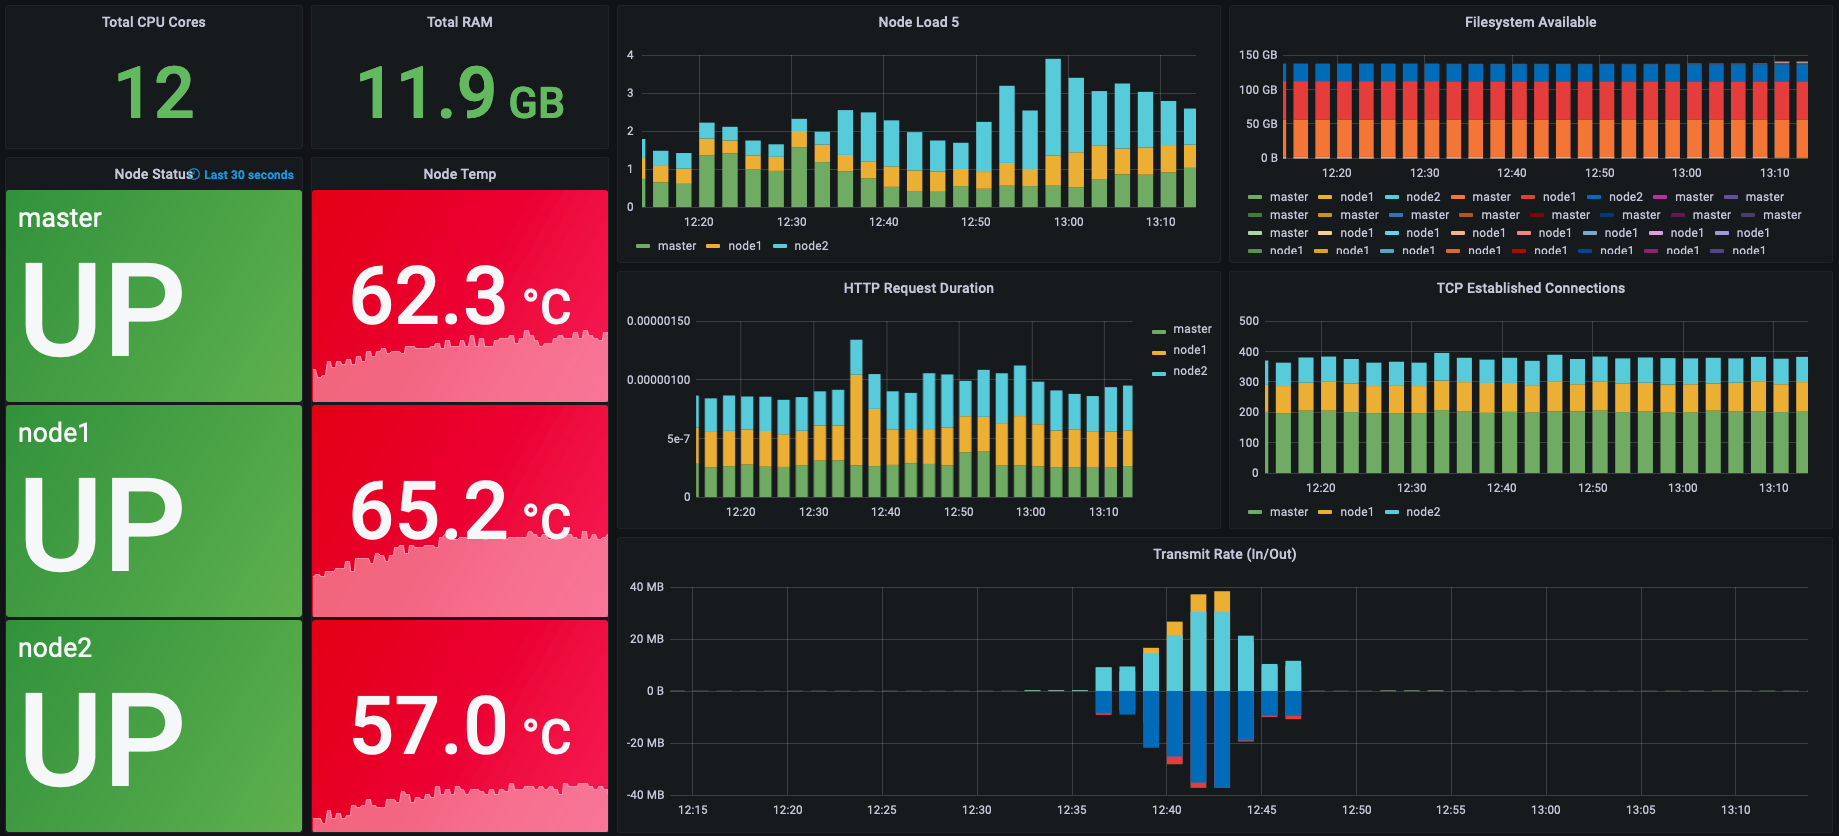
\includegraphics[width=\textwidth]{assets/k3s/screenshots/grafana-k3s-metrics.png}
    \caption{K3s metrics on Grafana dashboard.}\label{fig:k3s-grafana-k3s-metrics}
\end{figure}

Besides using Prometheus as data source, the internal InfluxDB from subsection \ref{subsubsec:k3s-database-service} can also be used to provide data for visualization in Grafana. Figure \ref{fig:k3s-grafana-sensor-temperature-png} shows the average temperature of all BMP280 sensors by requesting the values form the InfluxDB.

\begin{figure}[H]
    \centering
    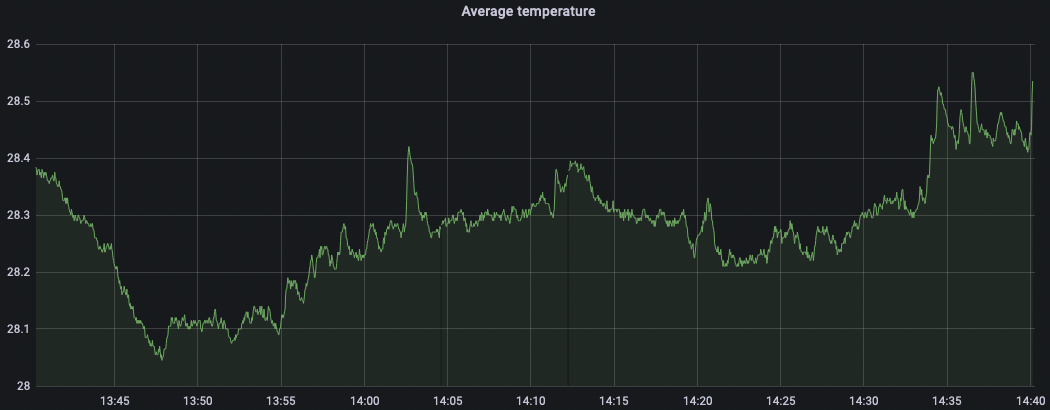
\includegraphics[width=\textwidth]{assets/k3s/screenshots/grafana-sensor-temperature-png.png}
    \caption{Average temperature of BMP280 sensors. Values provided by internal InfluxDB.}\label{fig:k3s-grafana-sensor-temperature-png}
\end{figure}

%%%%%%%%%%%%%%%%%%%%%%%%%%%%%%%%%%%%%%%%%%%%%%%%%%%%%%%%%%%%%%%%%%%%%%%%%%%%%%%%%%%%%%%%%%%%

\newpage
\section{AWS IoT Greengrass}
\gls{AWS} Greengrass consists of a cloud part running in the \gls{AWS} data centers around the world and a local part which runs on e.g. self owned hardware like a Raspberry Pi \cite{AmazonWebServicesHowItWorks}. It's important to note there are two versions of AWS IoT Greengrass and only version two (v2) is discussed here. Version two is the newer one and isn't compatible with the API's from version one \cite{aws-greengrass-guide}. Figure \ref{fig:aws-greengrass-how-it-works} shows the two parts of Greengrass and the connections between them. The core devices are the edge devices which act locally on generated data to e.g. run predictions, aggregation tasks and more. These tasks can be bundled inside so-called components, which then can be deployed to the Greengrass core devices. Supported component runtimes are AWS Lambda functions, Docker containers, native OS processes, or custom runtimes. \cite{AmazonWebServicesHowItWorks}. Some runtimes like Docker or Python are not installed by the Greengrass installer and have to be installed manually by the developer or script, if the use is desired. The cloud part consists of the AWS IoT Greengrass cloud service which manages the core devices and any other AWS service which can be used by the core devices.

\begin{figure}[H]
    \centering
    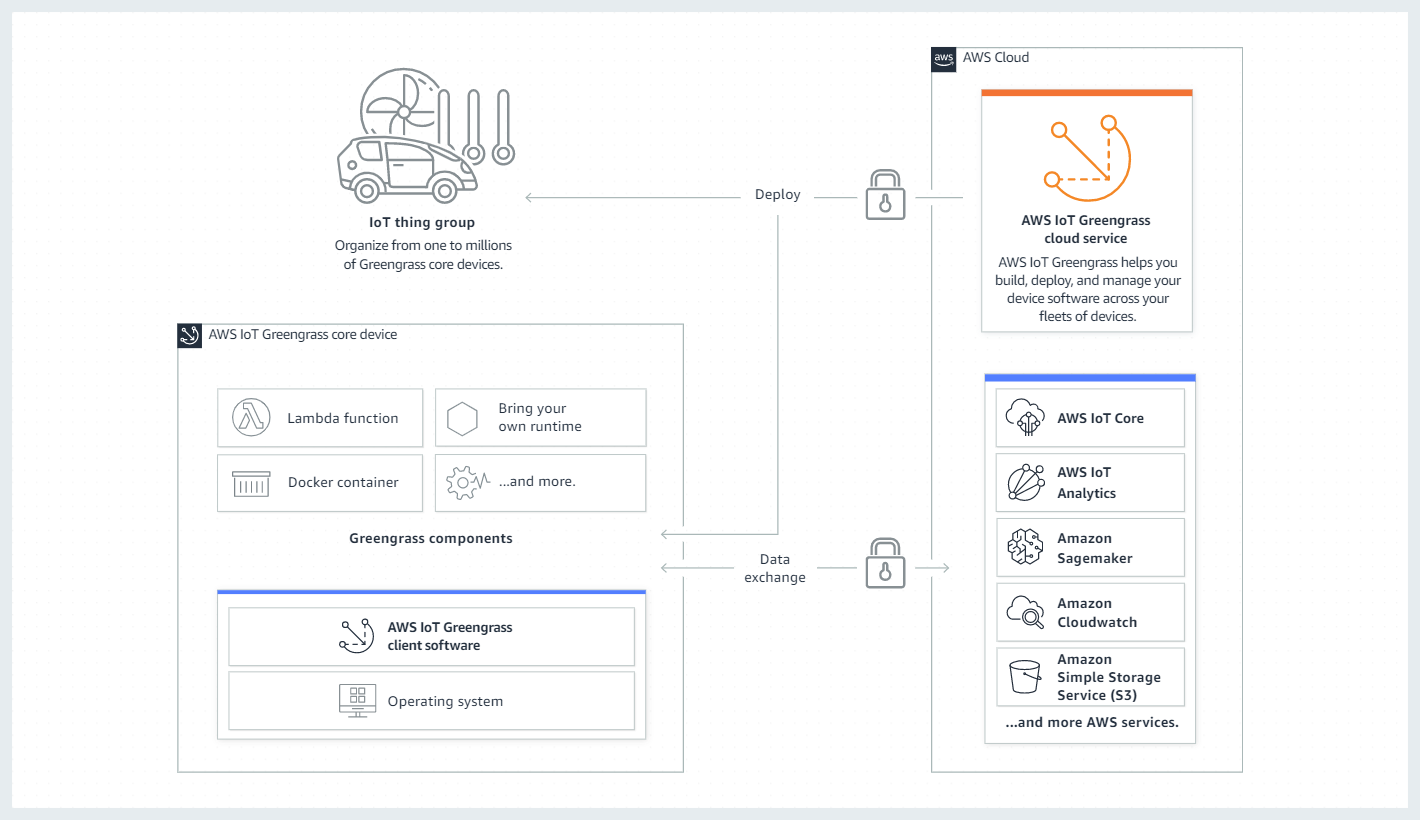
\includegraphics[width=\textwidth]{assets/aws-greengrass/aws-greengrass-how-it-works.png}
    \caption{AWS IoT Greengrass Architecture \cite{AmazonWebServicesHowItWorks}.}\label{fig:aws-greengrass-how-it-works}
\end{figure}

\paragraph{Greengrass core device:}
The core device is the device where edge computing ultimately takes place by running various components in different runtimes. Nearly everything can be deployed to the core device, like the \gls{AWS} Greengrass intro already mentions. For example, the core device contains an AWS provided MQTT broker which provides an interface for local IoT devices and allows them to directly publish and subscribe to the core device. The published messages can then be further processed by custom components directly on the core device \cite{AmazonWebServicesHowItWorks}.

\paragraph{Greengrass component:} Components are a software module that is deployed to the core device. This software module contains the executable software. Pre-built public components like the MQTT broker or log manager are provided by \gls{AWS}.
\cite{AmazonWebServicesHowItWorks}

\paragraph{Greengrass client device:} Client devices are the sensors/actors or generally the devices which connect to the core device for exchanging messages. Client devices do not need to know the direct address of the core device but can request it by means of a discovery process \cite{AmazonWebServicesHowItWorks}.

\paragraph{Greengrass cloud service:} The Greengrass cloud service is the cloud part which allows the developer to manage all the core devices and the distribution of Greengrass components \cite{AmazonWebServicesHowItWorks}.

\newpage
\subsection{Use case implementation}
The figure \ref{fig:aws-ggc-arch} below shows the implemented architecture and all the used components for the use case implementation. On the cloud side no services except the necessary ones were used. Inside the Greengrass core device the components are divided into AWS provided components and custom self written components. The MQTT protocol is used for communication between the cloud service and the core device. The client devices like the BMP280 and MQ2 sensor also use the \gls{MQTT} protocol to communicate with the core device. How the services on the core device were implemented will be explained in the following sections.

\begin{figure}[H]
    \fontsize{7}{10}\selectfont
    \centering
    \def\svgwidth{\textwidth}
    \input{assets/aws-greengrass/aws-greengrass-arch.drawio.pdf_tex}
    \caption{AWS Greengrass architecture overview.}
    \label{fig:aws-ggc-arch}
\end{figure}

\subsubsection*{Node setup}\label{subsubsec:aws-ggc-devices}
All three nodes were provisioned with the Ansible\footnote{\url{https://www.ansible.com/}} tool. The self written Ansible playbook follows the \gls{AWS} developer guide\footnote{\url{https://docs.aws.amazon.com/greengrass/v2/developerguide/quick-installation.html}} of installing the Greengrass Core with the \gls{AWS} provided installer. Besides the basic setup, which is explained in the developer guide, additional tools like Docker and Python get installed too. Before running the Ansible playbook against the configured devices the tool Terraform creates some \gls{AWS} resource like the device role, S3 bucket for storing artifacts and \gls{AWS} \gls{ECR} for storing private container images. After the Greengrass Core is installed on all configured devices, they will show up in the \gls{AWS} console under the Greengrass section in IoT Core. The devices contain only the basic components after the initial installation. By configuring the discovery feature for client devices, the \gls{AWS} provided components from figure \ref{fig:aws-ggc-arch} get installed on each core device of the same \textit{Thing group}. This discovery feature enables client devices to find and connect to discovered core devices. All devices which were set up from the example Ansible playbook are of the same \textit{Thing group}. The components get installed by creating and then triggering a deployment to the devices. Two of the components need configuring before deploying. The Auth component requires a JSON which describes which client devices are allowed to connect to the Greengrass Core device. The \gls{MQTT} bridge component also requires a JSON which describes the relaying of received and published messages. Example configuration JSON files can be found in the attached Git repository.

\newpage
\subsubsection*{Client devices}
All three devices BMP280, MQ2 and Ventilator need adjustments to connect to a Greengrass Core Device. At first, each new device needs to be registered as a \textit{thing} in the AWS Console. By registering the device, AWS allows the recommended certificate and key generation. This will generate a certificate and a public/private RSA key pair which is unique to each device. These certificates and keys are then used to authenticate the device against AWS and the Greengrass Core device. By registering a device, there is also the option of a \textit{policy}, which can be attached individually to each device. This policy provides information about what a device may or may not allowed to do. For this implementation the policy looks like the JSON in listing \ref{lst:iot-device-policy}. The policy in listing \ref{lst:iot-device-policy} allows the sensors and actors to connect, publish, subscribe and receive messages from the AWS IoT \gls{MQTT} broker. In addition to the \gls{MQTT} actions, the Greengrass action allows the device to discover local Greengrass core devices. Like the \textit{"Node Setup"} section in \ref{subsubsec:aws-ggc-devices} already mentions, the discovery feature must be enabled and configured before IoT device can connect to a local core device. Also, IoT devices must be manually added to the client devices list on each Greengrass core device to be able to discover the corresponding core device.

\begin{lstlisting}[caption={Client device policy.},label={lst:iot-device-policy},captionpos=b]
{
  "Version": "2012-10-17",
  "Statement": [
    {
      "Effect": "Allow",
      "Action": [
        "iot:Connect",
        "iot:Publish",
        "iot:Subscribe",
        "iot:Receive",
        "greengrass:*",
      ],
      "Resource": "arn:aws:iot:<region>:<account_id>:*"
    }
  ]
}
\end{lstlisting}

\subsubsection*{MQTT}
The communication with client devices works with an integrated MQTT broker. In addition to the MQTT broker is the MQTT bridge which is responsible to map MQTT messages to different messaging technologies. In total there are three different messaging technologies which cane be utilized by the Greengrass core devices. The first is the already mentioned MQTT broker, which provides the ability to publish and subscribe to specific MQTT topics. The second one is the \textit{PubSub} broker for local, device internal, publishing and subscribing. Local components can subscribe and publish to the PubSub broker by using \gls{IPC}. The third and the last one is the \textit{IoT Core} which simply transfers configured topics to the AWS IoT Core in the cloud for further use by e.g. \gls{AWS} cloud services. This option requires internet connection. Connection loses are ok due to the integrated queue, which will send the messages again after reconnect \cite{AmazonWebServicesMQTTBridge}. The MQTT bridge allows the developer to configure the mapping from one messaging technology to another. This configuration can be done during the deployment by providing an JSON configuration with all the required mappings. Listing \ref{lst:ggc-mqtt-bridge-configuration} shows the mapping of topic \textit{"sensor/\#"} form the MQTT broker, represented as \textit{LocalMqtt}, to the internal \textit{PubSub} broker.

\begin{lstlisting}[caption={Mapping messages from MQTT topic \textit{"sensor/\#"} to Pubsub broker.},label={lst:ggc-mqtt-bridge-configuration},captionpos=b]
{
  "mqttTopicMapping": {
    "SensorMapping": {
      "source": "LocalMqtt",
      "target": "Pubsub",
      "topic": "sensor/#"
    },
    ...
}
\end{lstlisting}


\subsubsection*{Detector service}
To also show the use of Docker container, the detector service was created and deployed as docker container. Unlike the detector service in the k3s example, a normal web server was used to receive an image instead of MQTT. The web server processes incoming POST requests at the REST endpoint \textit{/images} and publishes the machine learning results to the internal Greengrass core PubSub broker by using \gls{IPC}. To use \gls{IPC} inside a container, special environment variables, folders and policies must be added \cite{AmazonWebServicesDockerContainer}. The following list enumerates all required environment variables which need to be passed to the docker container to use \gls{IPC}.

\begin{itemize}
    \item \texttt{AWS\_REGION}
    \item \texttt{SVCUID}
    \item \texttt{AWS\_GG\_NUCLEUS\_DOMAIN\_SOCKET\_FILEPATH\_FOR\_COMPONENT}
    \item \texttt{AWS\_CONTAINER\_AUTHORIZATION\_TOKEN}
    \item \texttt{AWS\_CONTAINER\_CREDENTIALS\_FULL\_URI}
\end{itemize}

In addition to this list of environment variables, the container also needs access to the local Greengrass files to connect to the \gls{IPC} socket. This can be done by simply mounting the installation directory of Greengrass into the container. And finally the component requires a policy to be able to publish to the local PubSub broker. This policy can be added during the deployment phase by providing a default configuration with the corresponding policy, like shown in listing \ref{lst:ggc-detector-service-access-control-configuration}.

\begin{lstlisting}[caption={Access control configuration for publishing to IPC.},label={lst:ggc-detector-service-access-control-configuration},captionpos=b]
ComponentConfiguration:
  DefaultConfiguration:
    accessControl:
        aws.greengrass.ipc.pubsub:
            <component_name>:pubsub:1:
                operations: ["aws.greengrass#PublishToTopic"]
                policyDescription: "Allows access to PublishToTopic."
                resources: ["*"]
\end{lstlisting}

As before with k3s, the \gls{usb} device must also be mounted with \textit{privileged} rights into the container. All this necessary environment variables, folder mounts and special container flags can be added to the docker run command which is used inside the component to describe what the core device has to execute to successfully start the component. At the end it should be pointed out that the deployment of docker containers only works with docker images form the \gls{AWS} \gls{ECR} (public and private) or public images from the Docker Hub registry. For example, the GitLab private container registry cannot be used at the time of writting \cite{AmazonWebServicesDockerContainer}.


\subsubsection*{Emergency service}
To show different functionalities of Greengrass the emergency service was rewritten as \gls{AWS} Lambda function. The Lambda, serverless function, is developed by using the AWS provided \gls{SAM}\footnote{\url{https://aws.amazon.com/serverless/sam/}} command line tool. The function is simpler than its predecessor at the k3s example. The lambda is invoked by the Greengrass core for each message on the MQTT topic \textit{"sensor/\#"}. The topic which invokes the lambda is freely configurable on the Greengrass component creation. Each invoke will evaluate the incoming message and reacts to it by sending actor messages to the PubSub broker by using the \gls{IPC} socket\footnote{To access the IPC socket, the access configuration must be the same as for the detector service}. The used command line tool \gls{SAM} can be used to create the required ZIP file and to deploy this ZIP file to the \gls{AWS} cloud. After uploading the ZIP file, the serverless function will pup up in the \gls{AWS} console under \gls{AWS} Lambda. The Lambda can now be chosen during the Greengrass component creation process.

\bigskip
There is one problematic on developing these kinds of serverless functions. The CPU architecture is probably different from that of the Greengrass core device. In this example, the CPU architecture was different. By using python as runtime for the function most code works out of the box, but some libraries like the used \textit{awsiotsdk} uses native compiled code. For this case it must be ensured that the uploaded ZIP file only contains compatible native code or the lambda won't start on the core device. In this example implementation, the code must be compatible to the ARM processor architecture due to the usage of Raspberry Pi's.


\subsubsection*{Database service}
Greengrass core acts more as an intermediary entity for the processing of data and not for the storage of such data. Therefore, no database was deployed on the Greengrass core side. Sending results to the \gls{AWS} IoT Core and then storing them on e.g. a DynamoDB is an intended and viable solution. This doesn't mean deploying a database to the core device is not possible. There is no problem to deploying and connecting applications to a locally running database. This is just not an intended use case due to the missing redundancy.


\subsubsection*{Monitoring service}
Greengrass core devices continuously send status updates of the device itself and the running components. It is also possible to forward the local log files to \gls{AWS} CloudWatch by using the AWS provided component \textit{LogManager} \cite{AmazonWebServicesLogManager}. Therefore, no monitoring solution was developed due to the existing solutions.
        
\newpage
\section{ioFog}
ioFog is an edge computing platform for deploying, running, and networking distributed microservices at the edge. It is a management platform for managing microservices/applications on edge nodes \cite{ioFogCoreConcepts}. This is very similar to running microservices in a Kubernetes cluster, except in ioFog you have a very granular control of microservice deployment to selected agents. Microservices are packed inside container images and get then executed on the Docker container runtime \cite{ioFogArchitecture}. Figure \ref{fig:iofog-ecn-architecture} shows a basic architecture consisting of one control plane and two agents.

\begin{figure}[H]
    \centering
    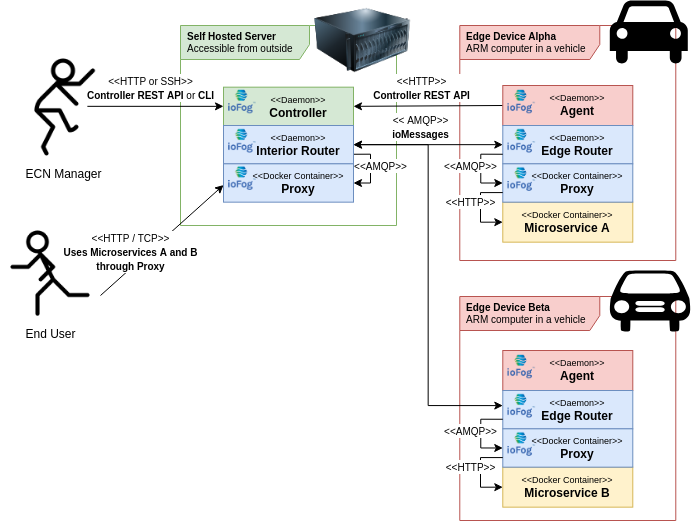
\includegraphics[width=\textwidth]{assets/iofog/iofog-architecture-ecn-router.png}
    \caption{ioFog Architecture \cite{ioFogArchitecture}.}\label{fig:iofog-ecn-architecture}
\end{figure}


\paragraph{Controller:} The controller is the master node of the \gls{ECN}. It orchestrates all agents, applications, microservices, and much more. The only requirement for the controller is the accessibility to it. Each agent, in the \gls{ECN}, needs access to the controller to get its instructions. A common solution is to deploy the controller to a cloud provider like \gls{AWS}, Microsoft Azure or Google Cloud Platform as the documentation suggests, but a local installation is also a viable solution. One node cannot contain both a controller and an agent daemon \cite{ioFogArchitecture}.

\paragraph{Agent:} The agent is the worker unit of the \gls{ECN}. Agents are typically deployed on the edge, e.g. near sensors, as native daemons. Each agent has the capability for running microservices, mounting volumes and managing resources. Microservices are represented as docker containers. An agent has not to be accessible from the outside, it only needs a connection to the controller. The agent receives instructions from the controller and also reports about its status \cite{ioFogArchitecture}.

\paragraph{Microservices:} Microservices are applications packed as Docker containers. Microservices get executed on the agent's Docker daemon \cite{ioFogArchitecture}.

\paragraph{Router:} The ioFog Router is an essential component that connects microservices together for communicating with the integrated messaging solution ioMessages. It also enables public port tunneling to microservices \cite{ioFogArchitecture}.

\paragraph{Proxy:} The Proxy is a microservice running on each agent. Its purpose is to translate HTTP requests to AMQP which is used by the routers as communication protocol \cite{ioFogArchitecture}.


\subsection{Use case implementation}
Figure \ref{fig:ioFog-arch} shows a simplified overview about the architecture built with the edge computing platform ioFog. Each yellow rectangle represents one agent of ioFog. The gray rectangle is the node with the control plane. Blue rectangles represent the on the node running docker engine.

\begin{figure}[H]
    \fontsize{6}{10}\selectfont
    \centering
    \def\svgwidth{\textwidth}
    \input{assets/iofog/iofog-arch-overview.drawio.pdf_tex}
    \caption{ioFog architecture overview.}\label{fig:ioFog-arch}
\end{figure}


\subsubsection*{Node setup}
All three nodes and the fourth node, which was added later, were provisioned with the \textit{iofogctl} command line tool. This tool is provided alongside ioFog to create and manage an ioFog \gls{ECN}. To provision a control plane or an agent, the command line tool requires the input of an YAML configuration file. This YAML file contains all information about the node itself and how to connect to it. Listing \ref{lst:ioFog-master-config} and listing \ref{lst:ioFog-agent-config} shows the entire configuration file used to provision the first control plane and the first agent. More configuration options can be found at the control plane and agent configuration YAML specification\footnote{\url{https://iofog.org/docs/2/reference-iofogctl/reference-control-plane.html}} \footnote{\url{https://iofog.org/docs/2/reference-iofogctl/reference-agent.html}}. Unlike the AWS Greengrass core installer, the \textit{iofogctl} command line tool installs all the required packages, like docker, on each node.

\bigskip
As the \gls{ECN} architecture figure \ref{fig:iofog-ecn-architecture} shows there two types of nodes, the control plane and the agents. The node with the control plane cannot contain an agent, therefore this setup includes one control plane and two agents respectively later three agents.

\noindent\begin{minipage}{.45\textwidth}
\begin{lstlisting}[caption={Control plane provisioning configuration.},label={lst:ioFog-master-config}]
---
apiVersion: iofog.org/v2
kind: ControlPlane
metadata:
  name: master
spec:
  controllers:
  - name: master-1
    host: 192.168.178.150
    ssh:
      user: ubuntu
      keyFile: ./keys/id_rsa
\end{lstlisting}
\end{minipage}\hfill
\begin{minipage}{.45\textwidth}
\begin{lstlisting}[caption={Agent one provisioning configuration.},label={lst:ioFog-agent-config}]
---
apiVersion: iofog.org/v2
kind: Agent
metadata:
  name: agent-1
  latitude: 46.204391
  longitude: 6.143158
spec:
  host: 192.168.178.151
  ssh:
    user: ubuntu
    keyFile: ./keys/id_rsa
\end{lstlisting}
\end{minipage}


\subsubsection*{Client devices}
The same implementation for the k3s client devices from subsection \ref{subsubsec:k3s-client-devices} can be used to connect to the MQTT broker on each agent. The only change which has to be made is the direct connection to one of the agents due to the missing load balancer, each client device is tied to exactly one agent.

\subsubsection*{MQTT}
The edge computing platform ioFog does not come with a built-in MQTT broker. Therefore, a MQTT broker was deployed as a ioFog application. The used MQTT broker, EMQX, is the same as the one in the k3s (\ref{subsubsec:k3s-mqtt}) example with one difference. Unlike the k3s MQTT brokers, the MQTT broker for each ioFog agent operates on a standalone basis and is therefore not in cluster mode. By exposing the ports of the broker client, like shown in listing \ref{lst:ioFog-mqtt-config} on line 73, devices can connect to the agent by using its IP address.

\begin{lstlisting}[caption={Example MQTT microservice configuration.},label={lst:ioFog-mqtt-config},captionpos=b]
apiVersion: iofog.org/v2
kind: Application
metadata:
  name: mqtt
spec:
  microservices:
    - name: mqtt-1
      agent:
        name: agent-1
      images:
        arm: docker.io/emqx/emqx:4.2.14
        registry: remote
      container:
        ports:
          - internal: 1883
            external: 1883 # <-- exposing MQTT port to the outside
    ...
\end{lstlisting}

One problem which occurs with this MQTT broker and the service on the same agent which want to subscribe to topics of the broker is that there is no possibility to directly connect to the MQTT broker. The \gls{MQTT} broker and any other application on the agent do not share the same network namespace, hence no direct connection can be established. Also, the ability to directly connect inside the Docker created network is not possible due to the container naming convention. The only way to connect to the MQTT broker is to connect over the agent's IPv4 address.


\subsubsection*{Detector service}
For ioFog the application from the k3s (\ref{subsubsec:k3s-detector}) example can be reused. Unlike in the k3s (\ref{subsubsec:k3s-detector}) example there is no need for specific selection of a node due to the fact that ioFog microservices are always specifically targeted to one agent only. The agent selection is always done by setting the agent name on the \textit{"agent.name"} attribute inside the YAML configuration. The agent selection is shown in listing \ref{lst:ioFog-detector-config} on line 6. Besides the agent selection, the \gls{usb} devices needs to be mounted into the container by attaching it as a volume like the listing \ref{lst:ioFog-detector-config} shows on the lines 12 to 15. Mounting the \gls{usb} device into the container requires the container to run in privileged mode, which is done by setting the \textit{rootHostAccess} attribute to \textit{true}, which is also shown in listing \ref{lst:ioFog-detector-config}.

\begin{lstlisting}[caption={Example detector microservice configuration.},label={lst:ioFog-detector-config},captionpos=b]
...
spec:
  microservices:
    - name: detector
      agent:
        name: agent-1
      images:
        arm: <detector-image>:<tag>
        registry: local
      container:
        rootHostAccess: true
        volumes:
          - hostDestination: /dev/bus/usb
            containerDestination: /dev/bus/usb
            accessMode: 'rw'
...
\end{lstlisting}

\subsubsection*{Emergency service}
Also the k3s emergency (\ref{subsubsec:k3s-detector}) version can be reused for ioFog. The service gets deployed on each of the agents and represents a standalone working unit. 

\subsubsection*{Database service}
Like \gls{AWS} Greengrass, ioFog is a more intermediary entity for the processing of data and not for the storage of such data. Therefore, no database is deployed on the agents. Sending results over the control plane to e.g. a Kubernetes cluster is an intended and viable solution. For the following section about the monitoring service, a InfluxDB was deployed to agent one.

\subsubsection*{Monitoring service}
A collection of services which represent the monitoring from subsection \ref{subsec:monitoring-service}. This collection includes the Telegraf\footnote{\url{https://www.influxdata.com/time-series-platform/telegraf/}} state metrics collector microservice, the time series database InfluxDB\footnote{\url{https://www.influxdata.com/}} and Grafana\footnote{\url{https://grafana.com/}} as visualization dashboard. The Grafana dashboard and the time series database are only deployed to a single agent (agent-1). The Telegraf microservice is deployed to both agents. Telegraf then collects metrics from the agent and the MQTT broker. The collected data will then be sent to the time series database on agent-1, which can be fetched from Grafana later on for visualization. To reach the Grafana dashboard from everywhere, its port is tunneled to the controller. By collecting all this data similar results like in the k3s figure \ref{fig:k3s-grafana-k3s-metrics} can be achieved.


%---- Evaluation
\chapter{Evaluation}\label{chap:evaluation}
This chapter contains the evaluation of each edge platform based on the explained evaluations criteria from chapter \ref{chap:evaluation-criteria}. This chapter is structured in such a way that the platforms receive an evaluation/assessment for each point individually while maintaining the order of the evaluation criteria from chapter \ref{chap:evaluation-criteria}.

%%%%%%%%%%%%%%%%%%%%%%%%%%%%%%%%%%%%%%%%%%%%%%%%%%%%%%%%%%%%%%%%%%%%%%%%%%%%%%%%%%%%%%%%%%%%
\subsection*{Access to peripheral devices}
\subsubsection*{k3s}\label{subsubsec:evaluation-peripheral-devices-k3s}
The edge computing platform k3s allows running applications access to the host/node hardware by running them in privileged mode. Privileged mode is not recommended and not necessary for the most containers. Example use cases which requires the container to run in privileged mode is the access to hardware like attached peripheral devices (e.g. \gls{usb} dongle). Containers which are running in privileged mode can perform all the capabilities that it's host can. In basic terms, running privileged containers is like running an application as root in the host, which grants the container direct access to the kernel, hardware resources and mounted disks which may result into a security risk \cite{DockerRunReference} \cite{Cardoso2020}. 

\bigskip
An alternative is a Kubernetes device plugin. Kubernetes provides a device plugin framework that can be used to provide access to system hardware resources by advertising it to the Kubelet. Vendors can implement a device plugin that gets deployed either manually or as a DaemonSet which can then be used by running pods \cite{KubernetesDevicePlugins}.

\subsubsection*{AWS IoT Greengrass}
AWS IoT Greengrass has three different kinds of running applications. Each of the three possibilities allows access to peripheral devices like a \gls{usb} device. The simple one is the execution directly on the host without any isolation techniques. In this scenario, the user who executes the component needs this permission to access the requested hardware. The second option is executing the component as serverless function (AWS lambda). To get access to a device outside the lambda environment, the configuration during the component creation needs to be adjusted. Respectively by creating a lambda Greengrass component, the option of adding devices is given. This option can be used to add specific device paths like the one for \gls{usb} (e.g. \textit{/dev/bus/usb}) to the lambda environment. This option also allows setting the permission to read-only or to read-write. By deploying a serverless function with such a configuration, the Greengrass core device will handle all the necessary steps for giving the lambda access to the configured peripheral device. The last and third option is running the component as Docker container. To access peripheral devices like \gls{usb} from the inside of docker containers, the container requires to be run with the privileged flag, which sets the container in privileged mode. The k3s section \ref{subsubsec:evaluation-peripheral-devices-k3s}, before this section, already describes the problems by running containers in privileged mode.

\subsubsection*{ioFog}
ioFog runs its applications as docker containers, therefore like the k3s evaluation section of this evaluation criteria already points out the container needs to be run in privileged mode to be able to access peripheral devices from the inside of a container. The k3s section \ref{subsubsec:evaluation-peripheral-devices-k3s} also describes the problems by running containers in privileged mode.

\bigskip
To prevent direct host access from the running application inside a container, ioFog provides extra microservices which serve as a \gls{HAL}. This moves the privileged mode from the application container to the \gls{HAL} microservice and makes the device accessible over the \gls{HAL} microservice \cite{ioFogHALMicroservice}.
%%%%%%%%%%%%%%%%%%%%%%%%%%%%%%%%%%%%%%%%%%%%%%%%%%%%%%%%%%%%%%%%%%%%%%%%%%%%%%%%%%%%%%%%%%%%
\subsection*{Data Persistence}
\subsubsection*{k3s}
Persisting data can be done like in any other Kubernetes cluster. One way of storing data on a Kubernetes cluster is to use persistent volumes. These volumes provide a persistent storage, but no redundancy across the entire cluster if they are set up with the default storage class. Redundancy can be achieved by using a different storage class \cite{KubernetesDocsPersistentVolumes}. In the documentation of k3s, the storage class Longhorn\footnote{\url{https://longhorn.io/}} is recommended for redundancy. Longhorn is an open-source distributed block storage system for Kubernetes and is not included in k3s. Therefore, Longhorn must be installed manually by using the shell command from listing \ref{lst:eval-k3s-pv} \cite{k3sDocsPersistentVolumes}.

\begin{lstlisting}[caption={Installing Longhorn to k3s cluster \cite{k3sDocsPersistentVolumes}.},label={lst:eval-k3s-pv},captionpos=b]
kubectl apply -f https://raw.githubusercontent.com/longhorn/longhorn/ master/deploy/longhorn.yaml
\end{lstlisting}

\subsubsection*{AWS IoT Greengrass}
AWS Greengrass core devices are not meant to permanently store data on their disk. Greengrass core devices are meant to transform and react to incoming data. To store data, a viable way is to transfer the data to the AWS cloud and store it there. In principle, it is not impossible to store data to the core device's disk. To be more clear, it is possible to store data on the core device's disk by either mounting a local path into a container/lambada or by writing files to the disk if the component is executed directly on the host without any abstraction/isolation. This kind of storing data on the Greengrass core device does not contain any redundancy or security measures.

\subsubsection*{ioFog}
The edge computing platform ioFog is not really meant to permanently store data on the agent's disk. Like AWS IoT Greengrass local volumes can be mounted to microservices but local volumes are not replicated and therefore do not support redundancy features. A viable way would be to send data, which needs to be permanently stored, to a cloud. Another viable solution would be to maintain a NAS server in the local network, which can be used by the agents to store data. 

%%%%%%%%%%%%%%%%%%%%%%%%%%%%%%%%%%%%%%%%%%%%%%%%%%%%%%%%%%%%%%%%%%%%%%%%%%%%%%%%%%%%%%%%%%%%
\subsection*{Development Environment}
\subsubsection*{k3s}\label{subsubsec:eval-development-environmemt-k3s}
Developing services for k3s is like developing services for any Kubernetes cluster, or generally developing containerized applications. A local development environment can be set up by either deploying k3s in virtual machines like EC2 instances on \gls{AWS} or by using a development tool called k3d. The virtual machine option is the closest to the production environment. K3s can be installed on the virtual machines in the same way as on, e.g. on Raspberry Pi's. Even the ARM architecture can be represented, e.g. by using AWS Graviton\footnote{\url{https://aws.amazon.com/ec2/graviton/}} EC2 instances. The second option is by using the tool k3d, which is provided by the k3s vendor himself. K3d allows the developer to install a k3s cluster on a single machine. K3d only requires Docker to be installed on the development machine \cite{RancherDocsAdvancedOptions}. Depending on the size of the k3s cluster, it can consume a lot of resources on the host machine. Deploying a subset of the services may help to improve the performance of the development machine.
    
\subsubsection*{AWS IoT Greengrass}
Developing services, or components as AWS Greengrass calls them, can be done in three different ways. The Docker option is like in k3s  (\ref{subsubsec:eval-development-environmemt-k3s}). The option of simply executing a binary or script on the host itself is also painless. The last option, AWS lambda, can be tricky to test and develop. If the target device, the Greengrass core device, uses an ARM based CPU architecture, the development of a lambda may needs some tricks to work. If the developed lambda uses any native code e.g. through a third party library, the uploaded ZIP needs to contain the ARM native binaries and not the x86 binaries. Even the by \gls{AWS} provided command line tool \gls{SAM} is not able to target a specific CPU architecture. \gls{SAM} always targets x86 machines. As a workaround, the compiled native code needs to be replaced by ARM compiled code. Another pain during the development is the testing of components which use \gls{IPC} to communicate with other services. There is no mock or anything which can be used to test the component. One option would be to develop and run the component on a local Greengrass core device.

\bigskip
A local Greengrass core device can be set up by either using a virtual machine or by using a local Docker daemon. Nevertheless, the local core device needs to be registered in the \gls{AWS} console as Greengrass core device \cite{AWSGGCInDocker}. Components can then be added to the device by using the Greengrass core command line tool on the core device.

\subsubsection*{ioFog}
The edge computing platform ioFog allows the developer to set up a local development environment by deploying the control plane and agents to a locally running Docker daemon \cite{ioFogLocalDeployment}. A deployment to any virtual machine or similar is also possible. Microservices in ioFog are containerized applications. There is also an SDK which enables the microservice to use the internal message routing of the so called ioMessages. To test sending and receiving of ioMessages, parts of the ioFog SDK must be mocked, or the testing takes place inside a development environment. 

%%%%%%%%%%%%%%%%%%%%%%%%%%%%%%%%%%%%%%%%%%%%%%%%%%%%%%%%%%%%%%%%%%%%%%%%%%%%%%%%%%%%%%%%%%%%
\subsection*{Extensibility}
\subsubsection*{k3s} New nodes can be added with ease. The master node contains the so-called \textit{node-token} which allows new nodes to join the cluster by using this token. The \textit{node-token} can be obtained on the master and needs then be used upon starting the agent on the new node like shown in listing \ref{lst:k3s-join-node} \cite{k3s}. This method requires a pre-installed k3s executable on the new machine. Another way, which was also done for this evaluation, is to add an additional IP address to the \textit{hosts.ini} file to provision it with the tool Ansible.

\begin{lstlisting}[caption={Joining new node to k3s cluster.},label={lst:k3s-join-node},captionpos=b]
    sudo k3s agent --server https://<master>:6443 --token ${NODE_TOKEN}
\end{lstlisting}

\subsubsection*{AWS IoT Greengrass}
Adding new core devices to AWS IoT Greengrass can be easily done by running the Greengrass core installer on the respective new device. If the installer specifies an existing "\textit{Things Group}" the new core device will join this group and automatically runs the deployment for this group. Like in the implementation section (\ref{subsubsec:aws-ggc-devices}) of \gls{AWS} Greengrass mentioned, runtimes like Docker or Python won't get installed by the Greengrass core installer and must be therefore installed manually.

\subsubsection*{ioFog}
To add a new agent/node to the ioFog \gls{ECN} a new configuration file must be created. The configuration file can then be executed using the ioFog command line tool. The command line tool will then install all the necessary components on the node and then adds it to the \gls{ECN}. Unlike AWS Greengrass the ioFog command line tool also installs all necessary runtimes. One problem which can occur by adding new agents to the \gls{ECN} is the rising amount of YAML configuration files needed. For example, a fleet of 100 devices results into at least 100 YAML configuration files for just deploying the agent's default deamon and services. Adding one microservice to each of the agents will result in 100 additional configuration files. This mess with that many configuration files is a problem but will be addressed in future version (v3.0) of ioFog which is currently in alpha state \cite{ioFogTemplateEngine}.

%%%%%%%%%%%%%%%%%%%%%%%%%%%%%%%%%%%%%%%%%%%%%%%%%%%%%%%%%%%%%%%%%%%%%%%%%%%%%%%%%%%%%%%%%%%%
\subsection*{Offline capability}
\subsubsection*{k3s}
The edge computing platform k3s can be fully operated in offline mode. At any point, from setting up the nodes to running applications, no internet connection is required at all. The cluster only needs a functional network to communicate with each other. Even new applications whose container images have not yet been downloaded do not need internet access. Container images can be pulled from a network reachable container registry. Therefore k3s can be operated completly offline.

\subsubsection*{AWS IoT Greengrass}
With AWS Greengrass fully offline capability is not given. Each core device gets instructions from the AWS data centers, and therefore a working internet connection is necessary. Also downloading/pulling new components during the deployment phase requires the Greengrass core devices to have access to the internet. The only offline capability which AWS Greengrass Core devices provide is the option to keep messages in a local queue until transmission is possible. This is optimal for edge devices which face internet outages from time to time. To sum it up AWS IoT Greengrass is not meant to run in environments where no internet connection is the norm.

\subsubsection*{ioFog}
Like the k3s edge computing platform, ioFog is able to operate fully offline. Which means, microservices can communictae with each other without any internet connection. New applications and their corresponding container images can be pulled from a container registry inside the local network. The only difference between k3s and ioFog, in the offline context, is the optional tree like network at ioFog which allows a network structure where the agents only need a connection to the control plane and not to each other agent inside the system.

%%%%%%%%%%%%%%%%%%%%%%%%%%%%%%%%%%%%%%%%%%%%%%%%%%%%%%%%%%%%%%%%%%%%%%%%%%%%%%%%%%%%%%%%%%%%
\subsection*{Cloud connectivity}
\subsubsection*{k3s}
Any kind of integrated cloud connectivity is not provided by k3s. But there are no restrictions on deploying nodes in the cloud. Therefore, it is possible to build a k3s cluster with a conjugation of edge and cloud nodes. The simultaneous deployment of nodes at the edge and in the cloud eliminates the advantage of the offline capability but enables other possibilites.

\subsubsection*{AWS IoT Greengrass}
Like the example implementation already shows, AWS Greengrass core devices are controlled from \gls{AWS} data centers. This deep integration of \gls{AWS} allows Greengrass components, which are running locally on a Greengrass core device, to interact with any \gls{AWS} service. An advantage of this deep integration is that separate credentials like the AWS Credentials are not necessary for interacting with AWS services. The component on the core devices authenticates itself by doing  mutual TLS (mTLS) with the X.509 certificate of the core device. Which services the Greengrass component can access depends on the IAM role assigned to the core device. AWS SDKs like the boto3 Python SDK automatically use this mechanism to access AWS services \cite{AWSGGCInteractWithServices}. Therefore, a combination of edge computing and cloud computing can be achived.

\subsubsection*{ioFog}
The edge computing platform ioFog does not provide any integrated cloud connectivity. On the other side, the ioFog documentation recommends deploying the control plane into the cloud. A conjungtion of cloud and edge is also possible as well as deploying everything to the edge \cite{ioFogArchitecture}.
%%%%%%%%%%%%%%%%%%%%%%%%%%%%%%%%%%%%%%%%%%%%%%%%%%%%%%%%%%%%%%%%%%%%%%%%%%%%%%%%%%%%%%%%%%%%
\subsection*{Service Differentiation}
\subsubsection*{k3s} 
By adding resource limits to a pod, a kind of prioritization can be achieved. It is possible to define the CPU shares, which gives the container access to a greater or lesser proportion of the host machine’s CPU cycles. Listing \ref{lst:k3s-service-differentation} demonstrates the request of the CPU share value of 1024 \cite{DockerDocsResourceConstraints} \cite{KubernetesResourceConstraints}. Besides the CPU share prioritization, a prioritization for preemption and scheduling can be defined for each pod. This priority indicates the importance of a pod relative to other pods. If a pod cannot be scheduled, the scheduler tries to preempt (evict) lower priority pods to make scheduling of the pending pod possible \cite{KubernetesPriorityAndPreemption}.

\begin{lstlisting}[caption={Running pod with the CPU share value of 1024.},label={lst:k3s-service-differentation},captionpos=b]
---
apiVersion: v1
kind: Pod
metadata:
  name: app
spec:
  containers:
    - name: app
    image: <container_image>:<tag>
    resources:
      requests:
        cpu: 1
\end{lstlisting}
    
\subsubsection*{AWS IoT Greengrass}
There is no built-in feature for giving Greengrass components different priorities. Different component priorities can be achieved by using the runtime environment options. By running components directly on the core device without abstraction/isolation, the scheduling priority can be modified by increasing or decreasing the niceness value of the corresponding process. Nicenesses range from -20 (most favorable scheduling) to 19 (least favorable) \cite{nice}. Docker containers can also be started with a type of priority. By adding the flag "\textit{--cpu-shares <number>}", like in listing \ref{lst:aws-service-differentation}, to the run command, Docker gives the container access to a greater or lesser proportion of the host machine’s CPU cycles \cite{DockerDocsResourceConstraints}.

\begin{lstlisting}[caption={Running Docker container with less shares than the default \cite{DockerDocsResourceConstraints}.},label={lst:aws-service-differentation},captionpos=b]
docker run -d --cpu-shares 512 <container_image>:<tag>
\end{lstlisting}
    
\subsubsection*{ioFog}
The possibility to specify CPU shares, like in k3s and AWS IoT Greengrass, is not possible for ioFog microservices. In general, there is no option to give a microservice any kind of prioritization relative to other microservices. The only prioritization which can be made is the priotiry attribute on each ioMessages. This assigned priority functions as a simple quality of service (QoS) indicator \cite{ioFogAgentReference}.
%%%%%%%%%%%%%%%%%%%%%%%%%%%%%%%%%%%%%%%%%%%%%%%%%%%%%%%%%%%%%%%%%%%%%%%%%%%%%%%%%%%%%%%%%%%%
\subsection*{Reliability}
\subsubsection*{k3s}
By unplugging one node, not the master/control plane, from the example setup, this node will be marked as \textit{"NotReady"} in the status field. The listing \ref{lst:k3s-unplug-node} shows the command line output while one worker node is unplugged.

\begin{lstlisting}[caption={Status of node 1 while unplugged.},label={lst:k3s-unplug-node},captionpos=b]
> kubectl get nodes
NAME     STATUS     ROLES                  AGE   VERSION
master   Ready      control-plane,master   5d    v1.21.1+k3s1
node1    NotReady   <none>                 5d    v1.21.1+k3s1
node2    Ready      <none>                 5d    v1.21.1+k3s1
\end{lstlisting}

Pods form the unplugged node (not ready) get moved to running nodes by recreating them. This can be seen by unplugging one node and then periodically fetching the pod states e.g. with \textit{kubectl}. Nodes which are specific to one node due to pod selection won't get recreated if there is no other pod which matches the given node selector. One must keep in mind that volumes are stored to the node disk itself, with the default storage class. To be able to move pods, which require persistent storage, a storage driver with redundancy support must be used.

\bigskip
The reliability of individual pods can be managed too. By adding liveness, readiness and startup probes for pods the cluster can detect failing pods.
In addition to the probes, a restart policy can be attached to a pod which tells the cluster on which failure events it should restart the pod. It defaults to restart the pod on each failure. This can be configured for each pod individually. Restarts happen with an exponential back-off delay (10s, 20s, 40s, …), that is capped at five minutes \cite{KubernetesPodLifecycle}.

\subsubsection*{AWS IoT Greengrass}
Failing Greengrass components or unavailable Greengrass core devices get marked as \textit{"UNHEALTHY"} in the AWS IoT Core Console. By loosing a Greengrass core device, the impact to the entire system depends on the system architecture. For example, a system for a postal service with one Greengrass core device on each delivery truck will result into entire lose of control for this truck. This is because no backup is available, so the control to this truck is lost until the core device reestablishes connection. A different example is the one which was built in the implementation section. Loosing one of the nodes, which was tested by unplugging one node, causes the sensors and actors to switch to healthy nodes. This switch can only be done if a healthy core device is in reach of the sensors which lost their initial core device.

\subsubsection*{ioFog}
The very granular control of microservice deployment to selected agents does not allow the move of microservices to healthy agents. To be more general, ioFog's agents do not work in cluster mode and therefore no auto recovery like in Kubernetes can be done. It's only possible to inform the system administrators about the failing/unavailable agent. Failing microservices are detectable over the ioFog API based on the status field. Sensor can switch the agen but the switching must be implemented by the developers.
%%%%%%%%%%%%%%%%%%%%%%%%%%%%%%%%%%%%%%%%%%%%%%%%%%%%%%%%%%%%%%%%%%%%%%%%%%%%%%%%%%%%%%%%%%%%
\subsection*{Security}
\subsubsection*{k3s}
Encryption is not used by default. For example, network encryption depends on the used \gls{CNI}. The default \gls{CNI} is VXLAN which is not encrypted. The following table \ref{tap:k3s-flannel-options} gives a brief overview of all available options to choose from for the \gls{CNI} including encrypted network options. Custom \gls{CNI}'s can be used too, but must be installed manually \cite{k3sNetworkOptions}. Encryption outside the cluster like the connection between the sensor to the MQTT broker, from the example implementation, must be enabled/configured by the developer themselves.

\begin{table}[H]
\centering
\begin{tabular}{|p{0.35\linewidth}|p{0.58\linewidth}|} \hline
    \textbf{CLI Flag and Value} & \textbf{Description} \\ \hline
    ---flannel-backend=vxlan     & (Default) Uses the VXLAN backend. \\ \hline
    ---flannel-backend=ipsec     & Uses the IPSEC backend which encrypts network traffic. \\ \hline
    ---flannel-backend=host-gw   & Uses the host-gw backend. \\ \hline
    ---flannel-backend=wireguard & Uses the WireGuard backend which encrypts network traffic. May require additional kernel modules and configuration. \\ \hline
\end{tabular}
\caption{Flannel backend CLI options \cite{k3sNetworkOptions}.}\label{tap:k3s-flannel-options}
\end{table}

\subsubsection*{AWS IoT Greengrass}
In AWS IoT Greengrass every communication, except the inter process communication between components on the core device, is encrypted. Each AWS Thing like a Greengrass core device have their own certificates and keys which get used on every communication step. The built-in MQTT broker only allows secure connections by default. In addition, the MQTT broker also requires the MQTT client to use mutual TLS (mTLS) protocol to authenticate them. Mutual TLS is also used by the Greengrass core devices for every communication from and to the cloud. The certificate from each device is attached to an AWS IAM role, which defines the operations allowed for AWS IoT devices \cite{AWSGGCEncryptionInTransit} \cite{AWSGGCDeviceAuth}.

\subsubsection*{ioFog}
The ioFog documentation does not mention any specific details about used security mechanism. By digging into the code of the agent\footnote{\url{https://github.com/eclipse-iofog/Agent/tree/v2.0.7}} and controller\footnote{\url{https://github.com/eclipse-iofog/Controller/tree/v2.0.1}}, the following security mechanism were found. The controller and agent communicate over HTTPS by using their self-signed certificates. The agent always pins the certificate on each request, which means it checks if the controller is really the one that it claims to be. Additionally, security guidelines are enforced and controlled by every node. Which guidelines are enforced and checked exactly are not further mentioned \cite{Marshall2019}. External communication is not secured by default and must be therefore done by the developer by e.g. using an MQTT broker in TLS mode.

%%%%%%%%%%%%%%%%%%%%%%%%%%%%%%%%%%%%%%%%%%%%%%%%%%%%%%%%%%%%%%%%%%%%%%%%%%%%%%%%%%%%%%%%%%%%
\subsection*{Real-time capability}
\subsubsection*{k3s}
The edge computing platform has no built-in messaging solution therefore normal HTTP request were made to meassure the overall latency. Two pods, ping and pong, were deployed on two different nodes of the k3s cluster to meassure the latency between them. Figure \ref{fig:k3s-latency} shows the meassureing results in milliseconds. Compared to its competitotrs the overall latency is highest of all of them. Therefore, a kind of real-time messaging is not possible/recommended with this latency.

\begin{figure}[H]
    \centering
    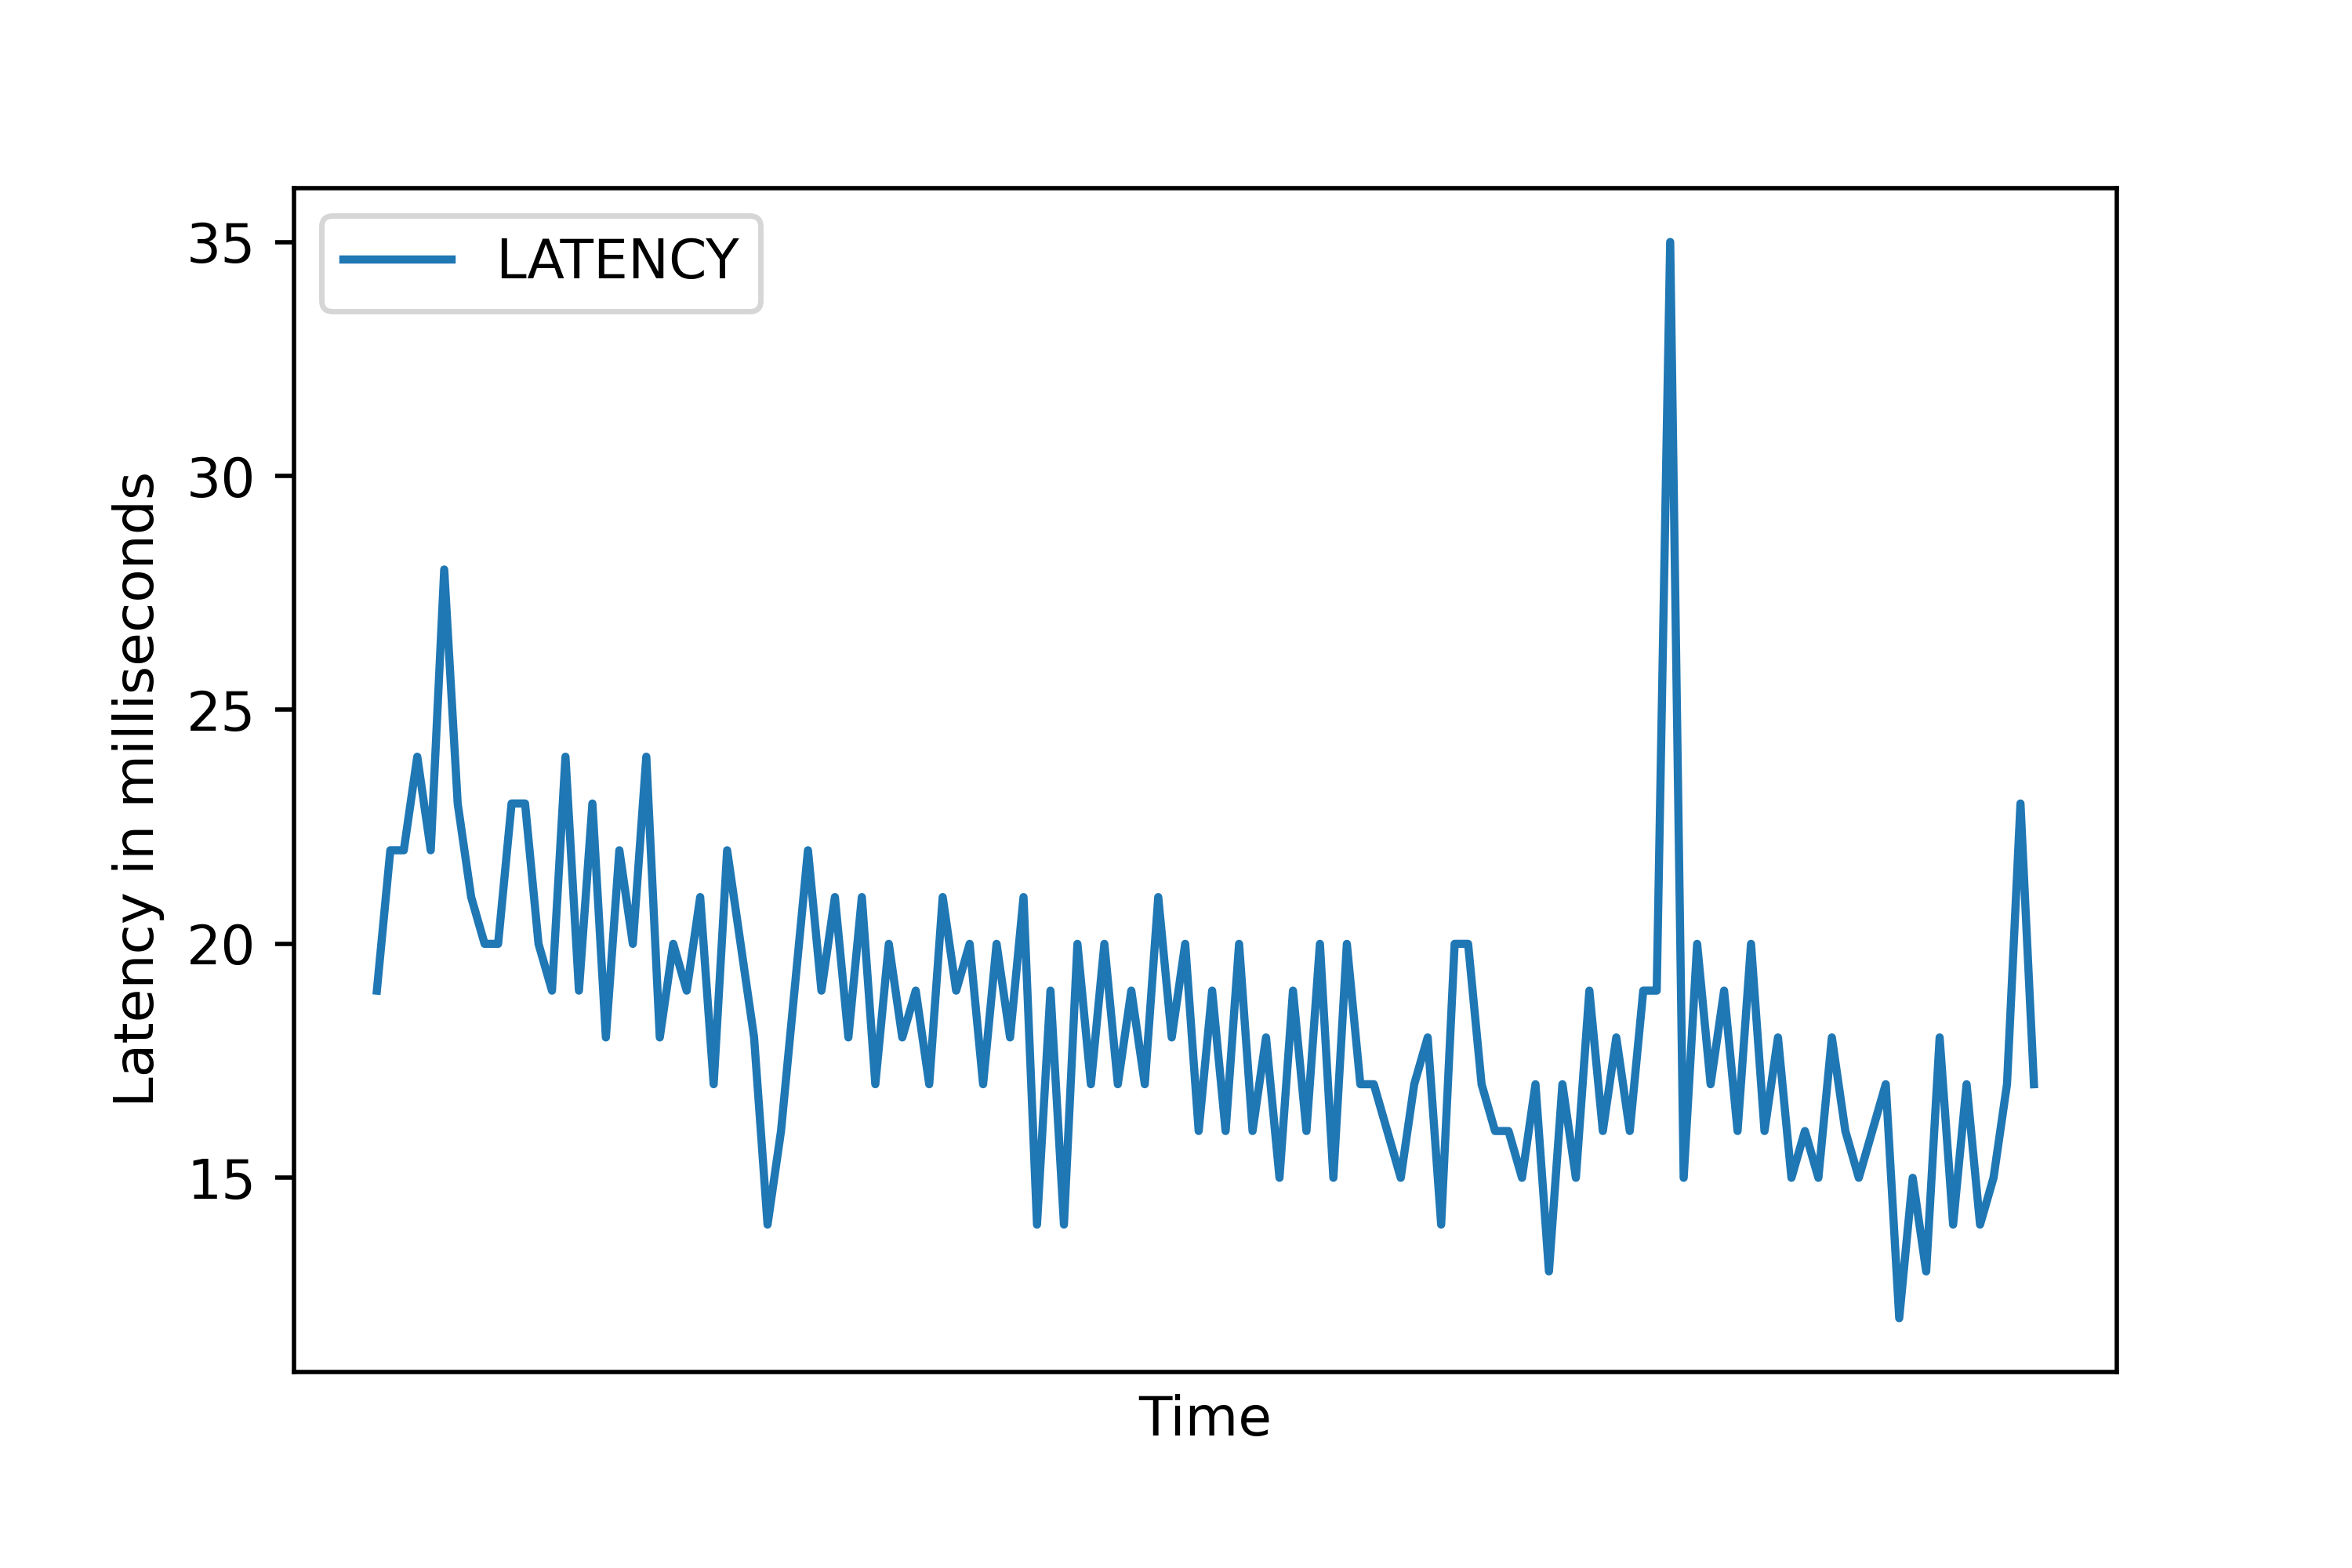
\includegraphics[width=0.8\textwidth]{assets/k3s/latency/plots/latency.png}
    \caption{HTTP latency between two pods on two nodes.}\label{fig:k3s-latency}
\end{figure}

\subsubsection*{AWS IoT Greengrass}
By using the \gls{IPC} provided on each Greengrass core device the latency is very low with some exceptions. Figure \ref{fig:aws-iomessage-latency} shows a message latency plot of two Greengrass components communicating over the built-in \gls{IPC} interface. Before the measuring was done, the core device got a fresh installation of the Greengrass core device components. The response time of around 4 milliseconds is good enough to deliver messages from high priority fast enough.

\begin{figure}[H]
    \centering
    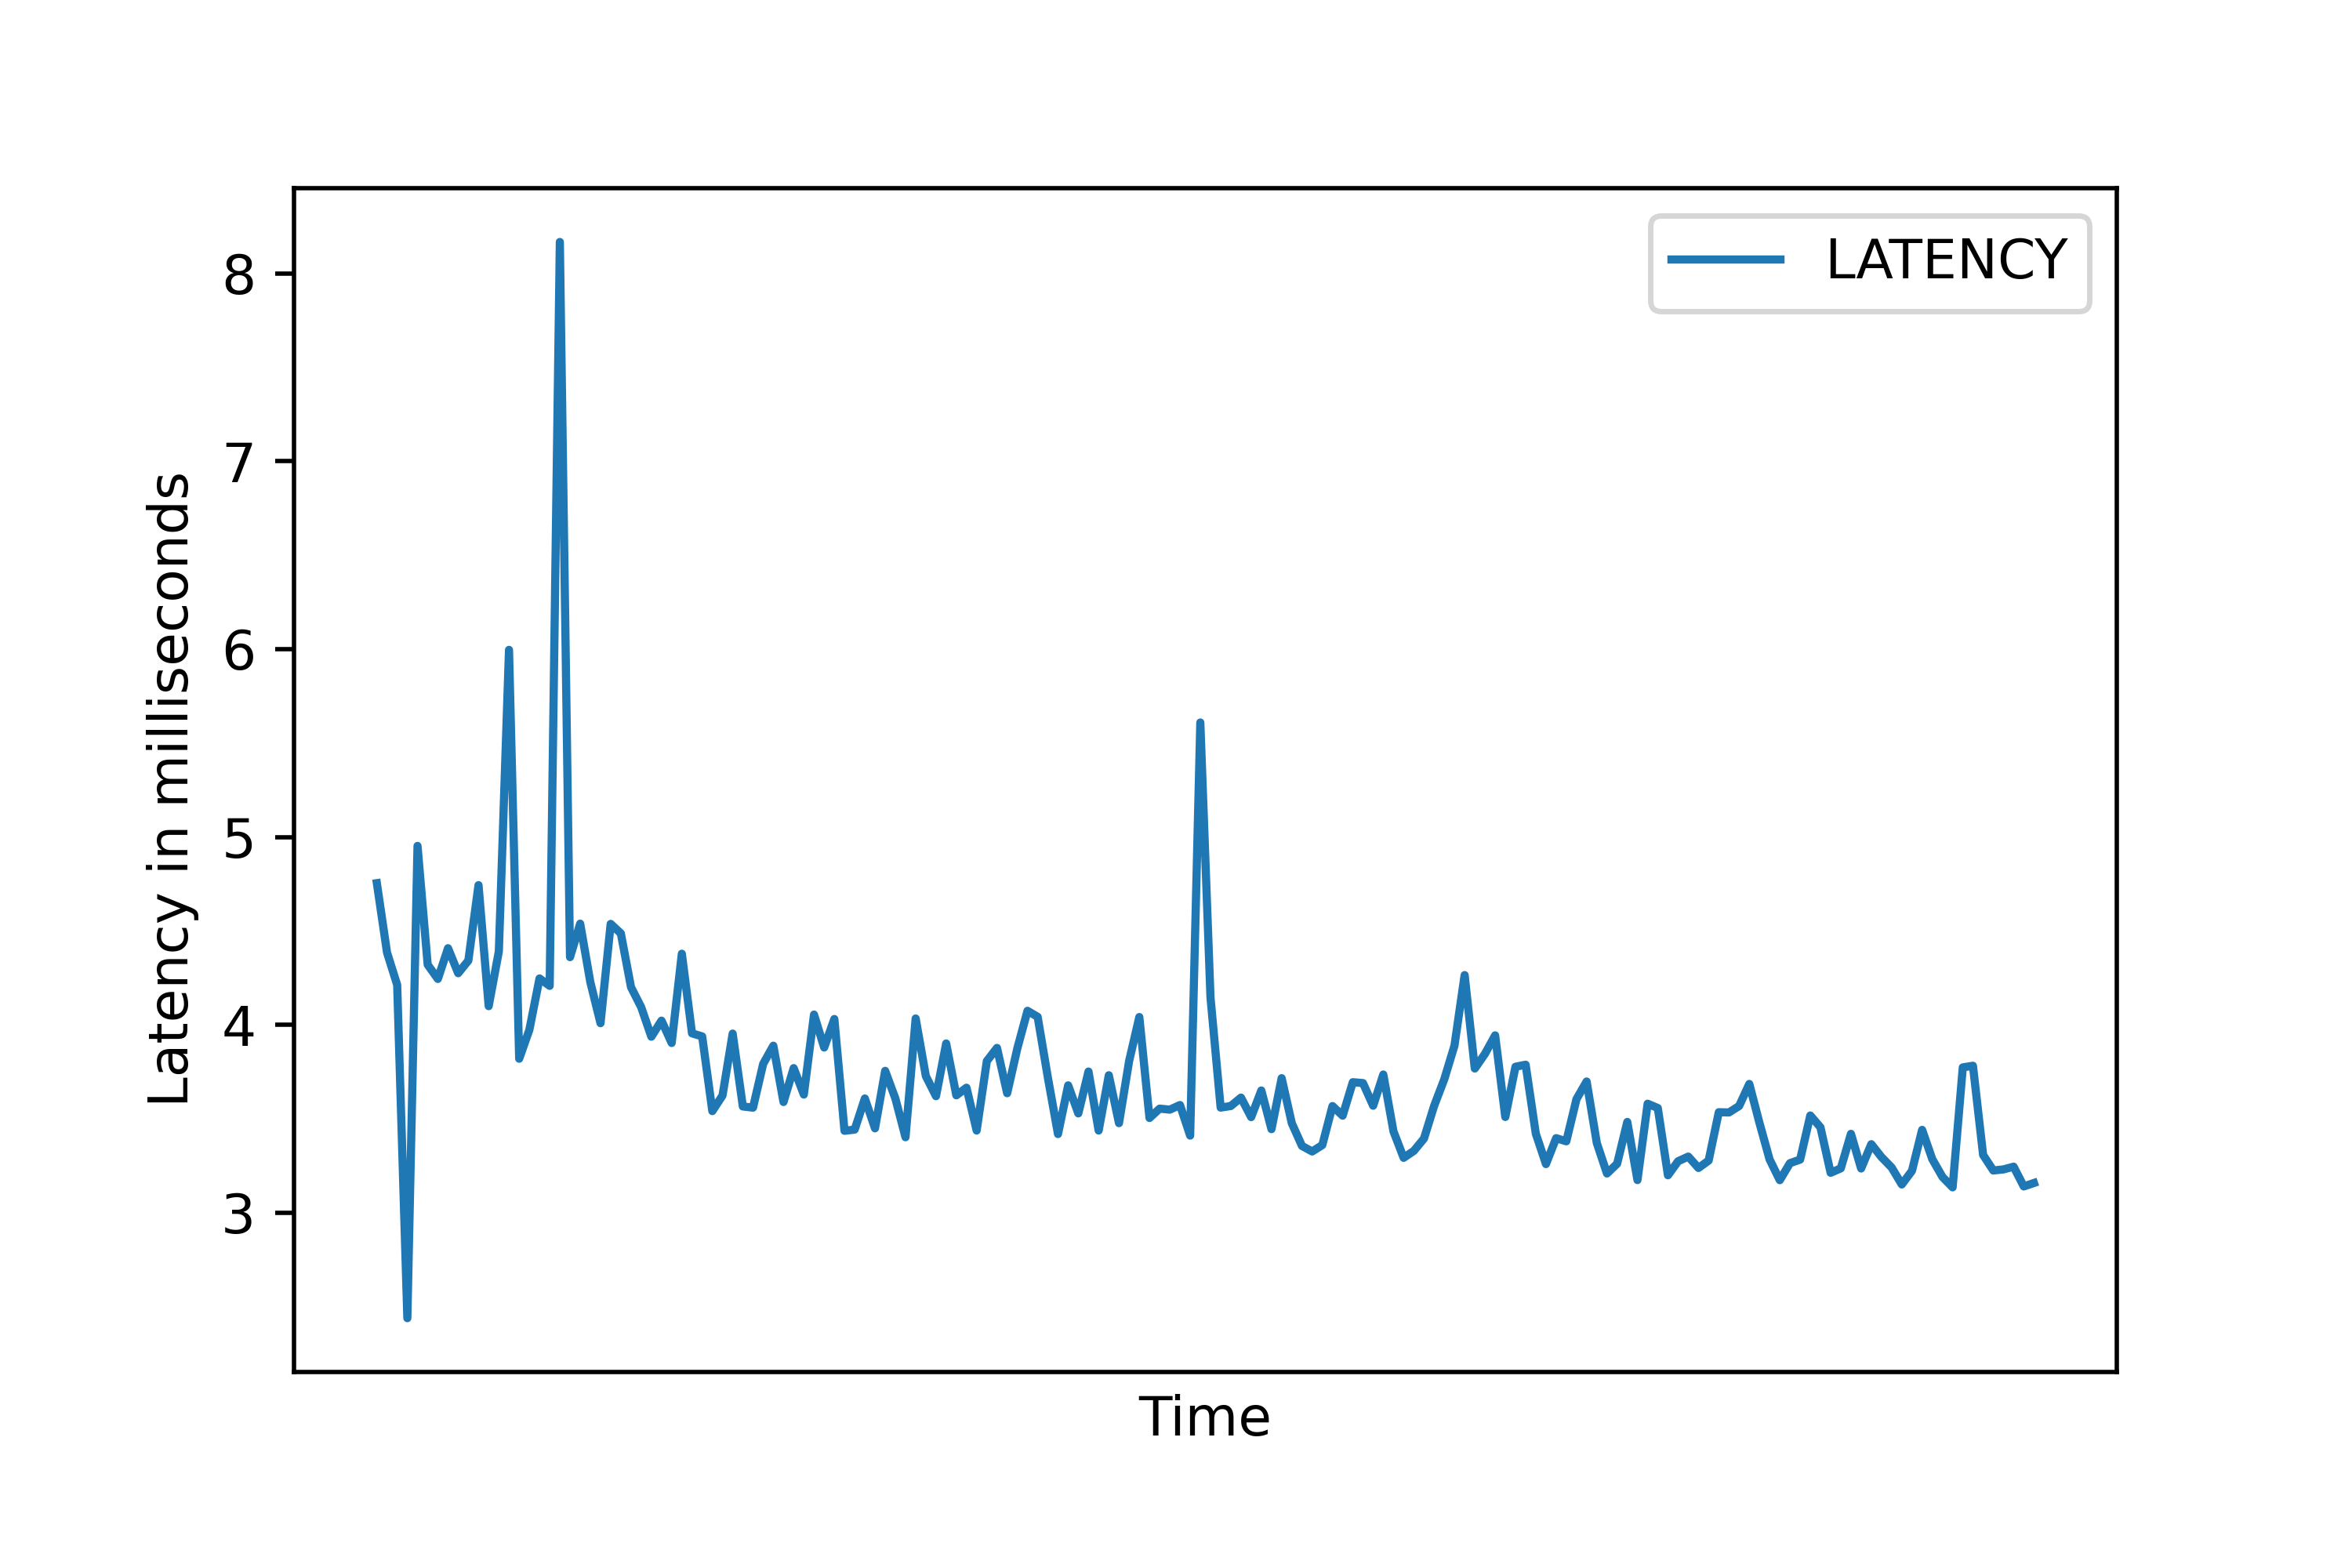
\includegraphics[width=0.8\textwidth]{assets/aws-greengrass/latency/plots/latency.png}
    \caption{IPC latency between two components on the same core device.}\label{fig:aws-iomessage-latency}
\end{figure}

\subsubsection*{ioFog}
By using the built-in messaging system of ioFog the latency can vary a lot like figure \ref{fig:ioFog-iomessage-latency} indicates. The recorded data points is the messaging time between two microservices on the same agent. Before the recording was done, the agent got a fresh installation of the ioFog agent services and daemons. The high spikes on an agent with just two microservices is not really promising on the real-time point of view. Therefore, a kind of real-time messaging is not possible/recommended with the native messaging system. Other options like communication inside the docker created network would make a better choice for a real time scenario.

\begin{figure}[H]
    \centering
    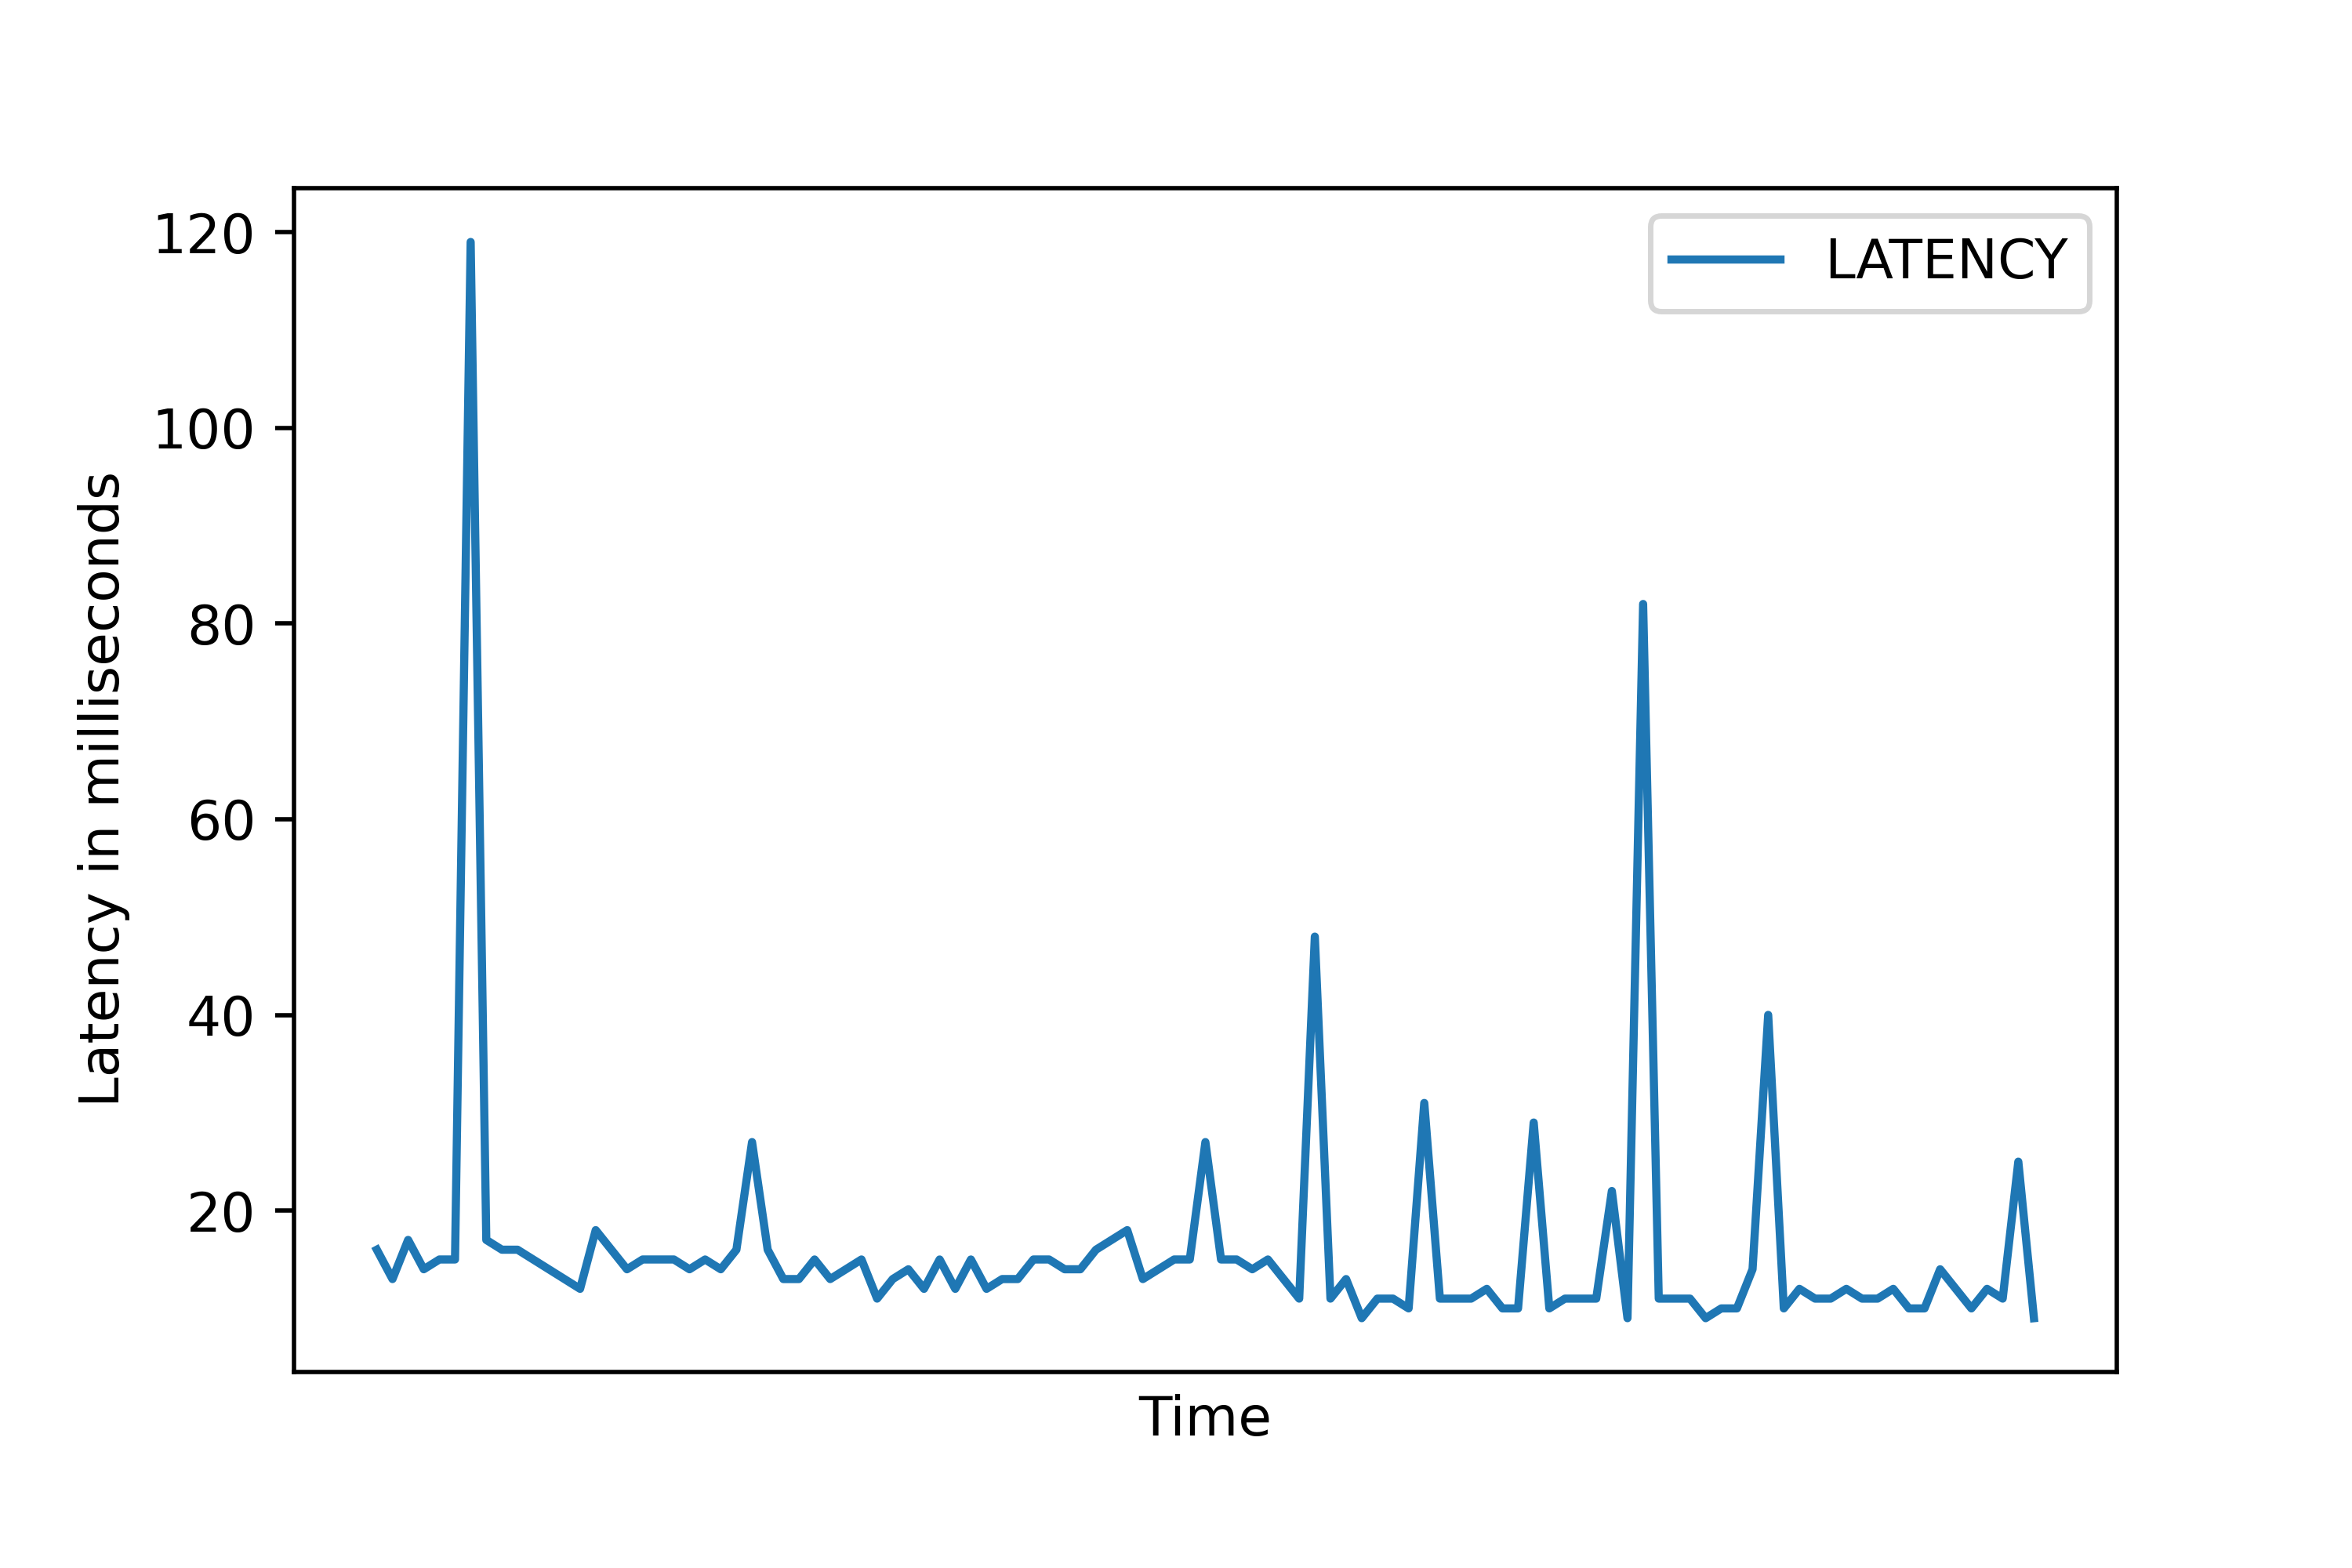
\includegraphics[width=0.8\textwidth]{assets/iofog/latency/plots/latency.png}
    \caption{ioMessage latency between two microservices on the same agent.}\label{fig:ioFog-iomessage-latency}
\end{figure}

%%%%%%%%%%%%%%%%%%%%%%%%%%%%%%%%%%%%%%%%%%%%%%%%%%%%%%%%%%%%%%%%%%%%%%%%%%%%%%%%%%%%%%%%%%%%
\subsection*{Performance}
Performance was measured by doing a fresh installation for each edge computing platform. No additional services were installed or added after the fresh installation. Performance is hard or even impossible to measure if it should be representative for each hardware. Therefore, an idling system was measured to show how much of the available resources each edge computing platform utilizes. The measuring was done with the Linux command line tool \textit{top}. The \textit{top} tool displays information about a selection of the active processes \cite{topUserManual}. The command from listing \ref{lst:performance-cli} was executed on each node for 15 minutes. The output file of the command from listing \ref{lst:performance-cli} was then transformed to draw the following plots.

\begin{lstlisting}[caption={Command to dump CPU and memory utilization.},label={lst:performance-cli},captionpos=b]
while true; do (echo "--- $(date)" && top -b -n 1 | head -n 5) >> ps.log; sleep 5; done
\end{lstlisting}

\subsubsection*{k3s}
The master node uses overall more memory and CPU time than the two worker nodes, as shown in figure \ref{fig:performance-k3s}. This is an expected behavior due to the fact that the master nodes contains several services to manage the cluster. The worker nodes utilize around the same amount of CPU and memory as expected. The usage of under 10\% of memory and CPU time, at the worker nodes, leaves plenty of resource for other services.

\begin{figure}[H]
    \centering
    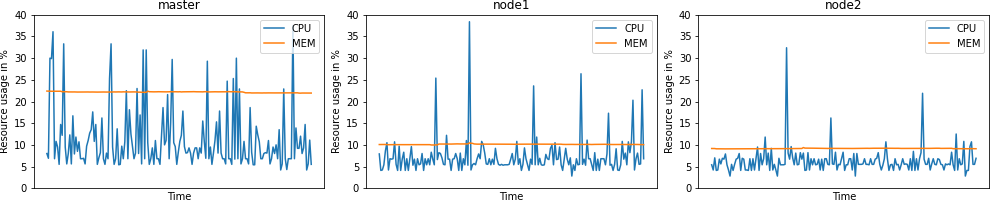
\includegraphics[width=\textwidth]{assets/k3s/logs/plots/results.png}
    \caption{CPU \& memory usage for the nodes master, node-1, node-2.}\label{fig:performance-k3s}
\end{figure}
    
\subsubsection*{AWS IoT Greengrass}
Each AWS Greengrass core devices contains the same set of services after a fresh installation, therefore the CPU and memory usage should be around the same amount. The plots in figure \ref{fig:performance-aws} confirm this assumption of nearly the same CPU and memory usage.

\begin{figure}[H]
    \centering
    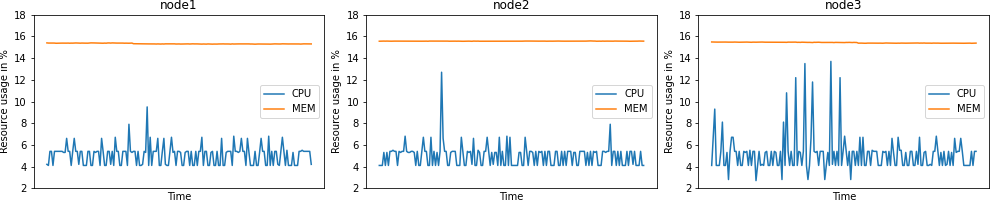
\includegraphics[width=\textwidth]{assets/aws-greengrass/logs/plots/results.png}
    \caption{CPU \& memory usage for the nodes node-1, node-2, node-3.}\label{fig:performance-aws}
\end{figure}

\subsubsection*{ioFog}
The CPU and memory usage across controller and agents seems to be around the same, as shown in the plots of figure \ref{fig:performance-ioFog}. The memory usage of around 20\% is high a may result into problems for memory intensive tasks compared to e.g. k3s.

\begin{figure}[H]
    \centering
    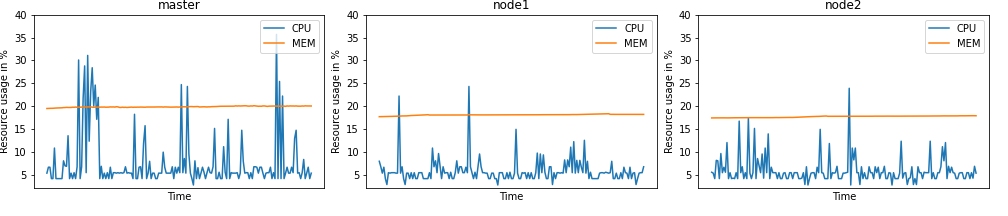
\includegraphics[width=\textwidth]{assets/iofog/logs/plots/results.png}
    \caption{CPU \& memory usage for the nodes master, node-1, node-2.}\label{fig:performance-ioFog}
\end{figure}

\subsubsection*{Summary}
The edge computing platform k3s seems to be the best in the category of the most balanced use of CPU and memory. The best in CPU is AWS IoT Greengrass closely followed by k3s. The most memory efficient platform is k3s. The ioFog edge computing platform seems to be the worst of all three, with its high memory usage and many high CPU usage spikes.

%%%%%%%%%%%%%%%%%%%%%%%%%%%%%%%%%%%%%%%%%%%%%%%%%%%%%%%%%%%%%%%%%%%%%%%%%%%%%%%%%%%%%%%%%%%%
\subsection*{Distributing workload}
\subsubsection*{k3s}
In short terms, its Kubernetes. The long explanation is the nature of Kubernetes and its workload distribution to all cluster nodes. Deploying an application into a Kubernetes cluster allows horizontal scaling. The horizontal scaling can be automated based on the load. This autoscaling feature of Kubernetes allows the system to dynamically react to increasing/decreasing demand of applications. By scaling up an application, creating replicas, the distribution to nodes is made by the kubelet. Mostly applications are normally not specifically targeted to one node, the kubelet then evenly distributes the applications to the available nodes in the cluster \cite{TheKubernetesAuthors}. 

\bigskip
One example of distributing workload at k3s is the MQTT broker cluster from the example implementation. The MQTT broker were deployed across all nodes to remain functional in the event of a node failure and also to get more computing resources if necessary. The workload was then distributed by adding a load balancer in front of the MQTT broker cluster. This load balancer evenly distributed all incoming connections to the available MQTT brokers.

\subsubsection*{AWS IoT Greengrass}
A distribution of workload is not the intention of AWS IoT Greengrass. Of course the distribution of workload can be implemented by the developer on their own, but this requires extra work to be done and isn't the default mode to compute things with AWS IoT Greengrass.

\subsubsection*{ioFog}
A distribution of workload is not the intention of ioFog. Doesn't mean it cannot be done. For example, having one agent which collects the sensor data in the area and distributes it to two nearby agents for the computational work. But this must be implemented by the developer and is not the default way.
%%%%%%%%%%%%%%%%%%%%%%%%%%%%%%%%%%%%%%%%%%%%%%%%%%%%%%%%%%%%%%%%%%%%%%%%%%%%%%%%%%%%%%%%%%%%
\subsection*{Energy Consumption}
For evaluating the overall energy consumption each system was measured for exactly one hour. One data point was recorded each second. Each platform was set up with three fresh installed nodes connected to the \gls{PoE} switch. The measuring was done on the \gls{PoE} switch power supply. Each system was idling and did not contain any custom applications or services, which do not come out of the box installed. Figure \ref{fig:energy-consumption-plot} presents the result from the experiment.

\begin{figure}[H]
    \centering
    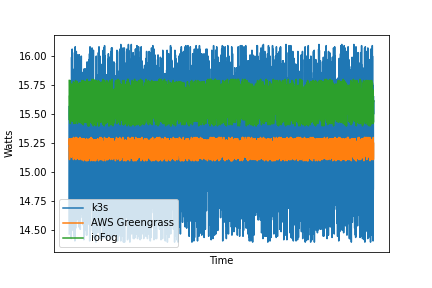
\includegraphics[width=\textwidth]{assets/evaluation/plots/energy-consumption.png}
    \caption{Energy consumption plot for all edge computing platforms.}\label{fig:energy-consumption-plot}
\end{figure}

\subsubsection*{k3s}
The energy consumption of k3s is varying a lot. Most of the energy is consumed by the node containing the control plane, as can be seen from the CPU and memory graphs in the first plot of the figure \ref{fig:performance-k3s} (the performance and energy consumption experiments were independent from each other).

\subsubsection*{AWS IoT Greengrass}
The AWS IoT Greengrass edge computing platform has the most consistent energy consumption of all platforms.

\subsubsection*{ioFog}
The power consumption of ioFog is very high compared to the rest considering that there are only two worker nodes available as the third is the designated to be the controller node.
%%%%%%%%%%%%%%%%%%%%%%%%%%%%%%%%%%%%%%%%%%%%%%%%%%%%%%%%%%%%%%%%%%%%%%%%%%%%%%%%%%%%%%%%%%%%
\subsection*{Cost}
Calculating the costs is more difficult than in the public cloud because hardware must be acquired, additional staff must be hired and more. The hardware cost also depends on the use case. For example, an edge computing use case which does a lot of machine learning task requires TPUs or GPUs which increases the cost where, on the other hand, sensor data processing requires less computing power which decreases the cost of hardware. And of course the size of the device fleet also plays an important role in the cost calculation.

\subsubsection*{k3s}
The costs are composed of the hardware and the additional staff members. Extra costs can be added if one of the node, e.g. the control plane, is deployed in a virtual machine at a public cloud like \gls{AWS}. But the entire system can be run locally without any cloud provider.
    
\subsubsection*{AWS IoT Greengrass}
Besides the hardware costs and the additional staff members, \gls{AWS} charges \$0.18\footnote{Price is taken from the region Europe(Frankfurt)} per month and Greengrass core device (price is varying depending on the region). Additionally, \gls{AWS} charges for AWS IoT Core connections e.g. transferring MQTT messages from and to the cloud, AWS \gls{S3} for storing application files, AWS \gls{ECR} for storing container images, and every other AWS services which is used by the core devices or components \cite{AWSGGCPricing}.

\subsubsection*{ioFog}
Like k3s the costs are composed of the hardware and the additional staff members. Agents or the control plane of ioFog can also be deployed to the cloud and will then generate additional cloud costs. But this is not necessary.
%%%%%%%%%%%%%%%%%%%%%%%%%%%%%%%%%%%%%%%%%%%%%%%%%%%%%%%%%%%%%%%%%%%%%%%%%%%%%%%%%%%%%%%%%%%%


%---- Conclusion
\chapter{Conclusion}
In the following paragraphs a conclusion to each edge computing platform and a general conclusion is given. At the end, a table with hints to which platform you could choose is given.

\paragraph{k3s:} There isn't much to say about k3s. It's simply an edge Kubernetes cluster. If you know Kubernetes you quickly find your way around. The downside of operating a Kubernetes cluster as edge computing platform is mainly the lack of default components which help the developers to e.g. connect local IoT devices. A big disadvantage of k3s is its development time which is highly increased, compared to the other two platforms, due to its lack of default components. On the other side, the biggest advantage of k3s is its versatility and the existing knowledge about Kubernetes among many developers. Compared to the other two platforms k3s has one big key difference to them. K3s is a network of worker nodes whereas the other platforms have individual worker units which are not meant to directly interact with each other.

\paragraph{AWS IoT Greengrass:} The AWS IoT Greengrass platform seems to be the most sophisticated solution of all. The possibility to run applications in various ways like Docker container or as lambda function allows the developer to choose the best option for case. Deploying and running applications on the core devices is made very easy and simple to understand. The ability to fine tune every component, for each core device, allows a wide variety of system control. But there are also downsides which should be kept in mind. For example the option to run applications as serverless functions could be frustrating in some parts. Especially if the developer tries to develop serverless functions for ARM core devices by using an x86 development environment or by using the \gls{AWS} provided tool \gls{SAM}. The most obvious disadvantage, which also includes an advantage in some scenarios, is the deep integration into the \gls{AWS} ecosystem. The advantage is given by the possibility of directly using a big variety of \gls{AWS} services in the cloud. Nevertheless, one must be aware that an extreme vendor lock then exists, which is the most concerning disadvantage. Also the offline capability is quite limited.

\paragraph{ioFog:} ioFog currently feels like an unfinished product. Problems like the mass production of configuration files for a big fleet creates a confusing overhead. Also, direct connections to other microservices is not possible. The IP address of the agent must always be used to connect to other microservices on the same agent. Upon request in the official ioFog community\footnote{\url{https://discuss.iofog.org/t/interservice-communication-with-http-mqtt-and-more/294}}, no statement could be made about this problem either. Some mentioned problems get resolved in future versions of ioFog. For example version 3.0 introduces a template engine for creating more agents and microservices without creating a new file for each \cite{ioFogTemplateEngine}.

\subsection*{Summary}
To sum it up, all three edge computing platforms are able to run workloads on the edge. Especially AWS IoT Greengrass is doing a great job on the edge but with a bade taste of vendor locking. 

On the exact other side is ioFog which lacks some features and is has some questionable methods for the overall configuration. This does not mean ioFog has no future but in its current state it is not recommended to use it in production grade environments. The newer and already announced version 3, which is currently in beta state, will resolve some of the concerns which appeared during this evaluation process. 

The platform k3s seems to be somewhere in the middle. On the one hand it is capable to do everything but on the other hand no default components or SDK's, which can speed up the development process, are given.
    

\subsection*{Which platform should you choose?}\label{subsec:which-platform}
The table \ref{tab:evaluation-matrix} below may help a developer to decide which platform suits their needs best. Some listed criteria are evaluated by the evaluation chapter \ref{chap:evaluation}. Other criteria which is not listed in the evaluation chapter \ref{chap:evaluation} are handpicked and maybe just important in some cases.


\bigskip
The colors in the table \ref{tab:evaluation-matrix} below have the following meaning: green indicates very good support of the corresponding platform, yellow means good to ok support, orange stands for bad support and red represents unsupported.

% ---------------------------------------------------------------
\begin{table}[H]
\centering
\begin{tabular}{|>{\columncolor[HTML]{CCCCCC}}r |>{\columncolor[HTML]{00FF00}}l |>{\columncolor[HTML]{00FF00}}l |l|}\hline
\multicolumn{1}{|l|}{\cellcolor[HTML]{4A86E8}} & \multicolumn{1}{c|}{\cellcolor[HTML]{4A86E8}k3s} & \multicolumn{1}{c|}{\cellcolor[HTML]{4A86E8}AWS} & \multicolumn{1}{c|}{\cellcolor[HTML]{4A86E8}ioFog} \\ \hline
Internode communication &  & \cellcolor[HTML]{FF9900} & \cellcolor[HTML]{FFFF00} \\ \hline
Interservice communication &  &  & \cellcolor[HTML]{FF9900} \\ \hline
Deploy to specific Nodes & \cellcolor[HTML]{FFFF00} & \cellcolor[HTML]{FFFF00} & \cellcolor[HTML]{00FF00} \\ \hline
Store data permanently and reliable &  & \cellcolor[HTML]{FF9900} & \cellcolor[HTML]{FF9900} \\ \hline
Cloud Support & \cellcolor[HTML]{FFFF00} &  & \cellcolor[HTML]{FFFF00} \\ \hline
Offline Support &  & \cellcolor[HTML]{FF9900} & \cellcolor[HTML]{00FF00} \\ \hline
No Vendor Lock &  & \cellcolor[HTML]{FF0000} & \cellcolor[HTML]{00FF00} \\ \hline
Battery operation & \cellcolor[HTML]{FF9900} &  & \cellcolor[HTML]{FFFF00} \\ \hline
Access to Hardware &  &  & \cellcolor[HTML]{00FF00} \\ \hline
Development Environment &  & \cellcolor[HTML]{FF9900} & \cellcolor[HTML]{00FF00} \\ \hline
Latency &  &  & \cellcolor[HTML]{FF9900} \\ \hline
SDK's & \cellcolor[HTML]{FF0000} &  & \cellcolor[HTML]{FF9900} \\ \hline
Cost &  & \cellcolor[HTML]{FF9900} & \cellcolor[HTML]{00FF00} \\ \hline
Monitoring &  &  & \cellcolor[HTML]{FF9900} \\ \hline
Big Fleet &  &  & \cellcolor[HTML]{FF9900} \\ \hline
Extensability &  &  & \cellcolor[HTML]{00FF00} \\ \hline
Workload distribution &  & \cellcolor[HTML]{FF0000} & \cellcolor[HTML]{FF0000} \\ \hline
Built-in secure communication & \cellcolor[HTML]{FFFF00} &  & \cellcolor[HTML]{FF9900} \\ \hline
\end{tabular}
\caption{Evaluation matrix for choosing the right platform.}\label{tab:evaluation-matrix}
\end{table}
% ---------------------------------------------------------------



%---- Outlook
\chapter{Outlook}
In conclusion, edge computing platforms support the operation and management of edge systems. Edge computing platforms mitigate or completely remove problems which can occur on IoT systems like the increased latency, increased bandwidth or privacy concerns. In the future, it remains to be seen how the platforms will develop, as some of them are still in an early stage of development.

\bigskip
In order to be able to assess the edge platforms even better, it would be appropriate to subject them to a longer field test in a real project. Further with the records of long term field tests better statements and decisions can be made about the practicability of the individual edge computing platforms. Also further research on how to connect existing IoT devices and factory machines into edge computing platforms should be done.

\bigskip
In the future, it will be interesting to see how existing systems with a large IoT devices base migrate to edge computing platforms and what complications arise. Currently, the problem is that the platforms sometimes feel more or less like alpha or beta. But it remains to be seen whether this will not change in the future. It also remains to be seen which edge computing platform companies prefer to choose in order to migrate existing systems or even create new systems. Finally, there is not only the choice between the platforms discussed in this thesis, but there are many more platforms including commercial platforms that have not been mentioned here at all. It therefore remains to be seen how the industry in general will adopt edge computing platforms.


%-------------------------------------------------------------------------------
% Bibliography
%-------------------------------------------------------------------------------
\backmatter
\listoffigures
\listoftables
\lstlistoflistings
\printglossary[type=\acronymtype, nonumberlist]
\printbibliography[heading=bibintoc]
\end{document} 
